\documentclass{report}
\usepackage[spanish]{babel}
\usepackage[utf8]{inputenc}
\usepackage{graphicx, longtable, float, titlesec, hyperref, enumitem, dingbat, multicol}
\usepackage[dvipsnames]{xcolor}
\usepackage[margin=2.75cm]{geometry}

\hypersetup{
    hidelinks = true
}

\titleformat{\chapter}[display]
  {\normalfont\bfseries}{}{0pt}{\Huge\thechapter.\space}

\titleformat{name=\chapter,numberless}[display]
  {\normalfont\bfseries}{}{0pt}{\Huge}

\titlespacing*{\chapter}{0pt}{-50pt}{20pt}

\begin{document}
    \begin{titlepage}
        \centering
        
\includegraphics[width=0.6\textwidth]{./img/logo.jpg}\\
        \vspace{1cm}
        \LARGE Software de Gestión de Empresa\\
        \vspace{0.5cm}
        \Large Ingeniería Informática de Gestión y Sistemas de Información\\
        \vspace{3cm}
        \Huge Proyecto de la asignatura\\
        \huge SoloG\\
        \vspace{2.5cm}
        \Large Autores:\\
        \vspace{0.2cm}
        \large Xabier Gabiña\\
        \large Ibai Sologuestoa\\
        \large Asier Cardoso\\
        \large Leire Becerra\\
        \vfill
        \today
    \end{titlepage}
    \tableofcontents
    \listoffigures
    \listoftables
    \chapter{Análisis del sector}
      \paragraph*{}{El sector industrial de la videovigilancia es una parte de la industria de la seguridad y la tecnología. Se encarga de proporcionar sistemas de vigilancia visual para una amplia gama de aplicaciones en entornos industriales y domesticos, como fábricas, almacenes, instalaciones de energía, plantas de producción, hogares, entre otros.}
      \section{Mercado objetivo}
        \paragraph*{}
        {
          El mercado objetivo de la videovigilancia es muy amplio y abarca desde la empresa hasta el hogar. 
          Aun así, el mayor volumen de ventas se da en el sector empresarial, donde se requieren sistemas de videovigilancia para proteger las instalaciones, controlar el acceso de personal y vehículos, y prevenir robos y actos vandálicos.
          Dentro del sector empresarial, se ha registrado un aumento en la demanda de sistemas de videovigilancia en el segmento de \textbf{infraestructuras críticas}, como aeropuertos, estaciones de tren, puertos, centrales eléctricas, entre otros.\cite{mordor-video-surveillance}
        }
        \paragraph*{}
        {
          Hay que tambien tener en cuenta que la demanda no es la misma en todos los países. La videovigilancia tiene un mayor peso en países como \textbf{Estados Unidos}, \textbf{China}, \textbf{Reino Unido}, \textbf{India} y \textbf{Brasil}, donde se han registrado un mayor número de instalaciones de sistemas de videovigilancia.\cite{mordor-video-surveillance}
        }
        \paragraph*{}
        {
          Tambien se espera que \textbf{Asia Pacífico} sea la región con mayor crecimiento en el mercado de la videovigilancia en los próximos años, debido al concepto de ciudades inteligentes ampliamente extendido especialmente en \textbf{China} y la creciente urbanización en la región.\cite{mordor-video-surveillance} \cite{bbc-videovigilancia} \cite{elpais-videovigilancia}
        }
        \begin{figure}[H]
          \centering
          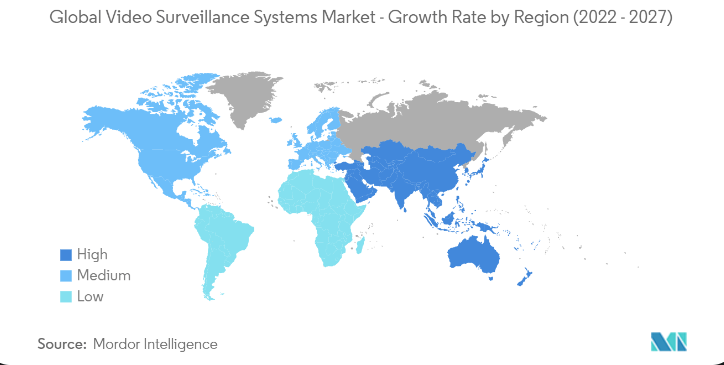
\includegraphics[width=0.7\textwidth]{./img/ssm.png}
          \caption{Mercado de la videovigilancia en 2022-2027}
        \end{figure}   
        \paragraph{}{
          Es por esto, que hemos decidido que el mercado objetivo de SoloG sea el sector empresarial, especializado en ofreces servicios con un enfoque especial en infraestructuras críticas y empresas de tamaño mediano y grande de los paises de Asia Pacífica, especialmente China, Japon y Corea del Sur debido a su alto crecimiento en el mercado de la videovigilancia.
        }
        \subsection*{Productos}
          \paragraph*{}
          {
            Los productos ofertados en el sector de la videovigilancia son muy variados.
            Incluso cerrando el foco en el sector empresarial, hay una amplia gama de productos que se pueden ofrecer a los clientes.
            Algunos de los productos más comunes son: \cite{wiki-videovigilancia-ip} \cite{illustra-cameras} \cite{prosegur-aiot}
          }
          \begin{multicols}{2}
            \begin{itemize}
              \item Cámaras de video
              \item Grabador de vídeo 
              \item Video Server Encoder
              \item Software de análisis de vídeo
              \item Dispositivos de visualización
              \item LED infrarrojos
              \item Sensores
              \item Reconocimiento Facial
            \end{itemize}
          \end{multicols}
        \subsection*{Servicios}
          \paragraph*{}
          {
            Los servicios ofertados en el sector de la videovigilancia, al igual que los productos, son varios y van desde la consultoría en seguridad hasta la instalación y mantenimiento de sistemas de videovigilancia. 
            Algunos de los servicios más comunes son: \cite{wiki-videovigilancia-ip}
          }
          \begin{itemize}
            \item Consultoría en seguridad
            \item Diseño e instalación de sistemas
            \item Mantenimiento preventivo soporte técnico
            \item Capacitación y formación
            \item Servicios de monitoreo y respuesta a alarmas
          \end{itemize}
        \subsection*{Competidores}
          \paragraph*{}{Debido a que el mercado de la videovigilancia se actualiza constantemente los actores del mercado fluctuan mucho y son altamente competitivos. Los competidores más importantes en el mercado de la videovigilancia en la actualidad son:}
          \begin{multicols}{3}
            \begin{itemize}
              \item Axis Communications AB
              \item Bosch Security Systems Incorporated
              \item Honeywell Security Group
              \item Samsung Group
              \item Panasonic Corporation
              \item Schneider Electric SE
            \end{itemize}
          \end{multicols}
          \paragraph*{}{Como hemos comentado, el mercado de la videovigilancia es muy competitivo, lo que significa que \textbf{no es un mercado consolidado} por lo que se podria llegar a entrar y competir en el con una buena estrategia.}
          \begin{figure}[H]
            \centering
            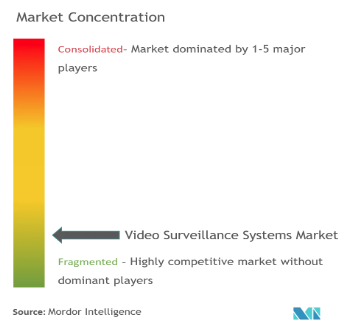
\includegraphics[width=0.4\textwidth]{./img/competidores.png}
            \caption{Competidores en el mercado de la videovigilancia}
          \end{figure}
          \paragraph*{}{Los competidores más importantes en el mercado de la videovigilancia son centrandono en el sector empresarial de Asia Pacífico son:}
          \begin{multicols}{2}
            \begin{itemize}
              \item Hikvision
              \item Dahua
              \item Axis Communications
              \item Samsung Group
            \end{itemize}
          \end{multicols}
        \subsection*{Proveedores}
          \paragraph*{}
          {
            Los proveedores de materias para la fabricación de productos de videovigilancia se pueden clasificar en dos categorías, proveedores de componentes electrónicos y proveedores de software. 
            Algunos de los proveedores más importantes de componentes electrónicos son \textbf{Canon}, \textbf{Axis}, \textbf{Milestone} y \textbf{BCD}. 
            Algunos de los proveedores más importantes de software son \textbf{EarthCam} e \textbf{Infotech}
          }
        \subsection*{Clientes}
          \paragraph*{}{
            Hay muchos clientes potenciales en el mercado de la videovigilancia, desde empresas y organizaciones hasta hogares y propietarios de pequeños negocios.
            Como hemos comentado previamente, nuestro objetivo es el de centrarnos en las infraestructuras críticas y empresas de tamaño grande.
            Un listado de clientes objetivos seria:
          }
          \begin{multicols}{2}
            \begin{enumerate}
              \item Empresas de energía
              \item Aeropuertos
              \item Estaciones de tren
              \item Puertos
              \item Bancos
              \item Edificios gubernamentales
            \end{enumerate}
          \end{multicols}
      \clearpage\section{Competidores}
        \paragraph*{}{
          Debido a que el mercado de la videovigilancia es muy competitivo, las empresas deben competir en precio, calidad, innovación y servicio al cliente para mantener o aumentar su cuota de mercado.
          Los principales productos y precios que manejan nuestros competidores son:
        }
        \begin{longtable}{|p{4cm}|p{5cm}|p{3cm}|p{3cm}|}
          \hline
          \textbf{Empresa} & \textbf{Productos} & \textbf{Precio/Unidades Venta} & \textbf{Precio/Unidad Producción}\\
          \hline
          \hline
          Hikvision & Cámaras de seguridad & 120€/u & 50€/u\\
          \hline
          Hikvision & Detector de inividores & 50€/u & 20€/u\\
          \hline
          Hikvision & Paneles de control & 200€/u & 100€/u\\
          \hline
          Dahua & Cámaras de seguridad & 100€/u & 40€/u\\
          \hline
          Dahua & Grabadora de video & 400€/u & 200€/u\\
          \hline
          Axis Communications & Cámaras de seguridad & 150€/u & 60€/u\\
          \hline
          Axis Communications & Intercomunicadores & 100€/u & 40€/u\\
          \hline
          Axis Communications & Panel de control de acceso & 300€/u & 150€/u\\
          \hline
          Axis Communications & Grabadora de video & 500€/u & 250€/u\\
          \hline
          \caption{Listado de productos de los competidores}
        \end{longtable}
        \begin{longtable}{|p{5cm}|p{11cm}|}
          \hline
          \textbf{Empresa} & \textbf{Servicios}\\
          \hline
          \hline
          Dahua & Software de análisis facial\\
          \hline
          Axis Communications & Software de análisis facial\\
          \hline
          Axis Communications & Servicio de monitoreo remoto\\
          \hline
          Axis Communications & Servicio de analisis de video\\
          \hline
          \caption{Listado de servicios de los competidores}
        \end{longtable}
        \paragraph*{}{
          En el caso de los servicios es muy complicado establecer un precio ya que estos dependen en gran medida de las necesidades del cliente y de la complejidad de la instalación por lo que son presupuestos hecho a medida.
          }
      \clearpage\section{Proveedores}
        \paragraph*{}{
          Dado el mercado en el que trabajamos, los proveedores son muchos y variados y dado el gran volumen de nuestra empresa necesitamos varios proveedores para poder abastecernos de los componentes necesarios para la fabricación de nuestros productos.
        }
        \paragraph*{}
        {
          Esta es la lista de proveedores con los que trabajaremos para obtener los productos que ofreceremos a nuestros clientes junto a nuestros servicios:
        }
        \begin{longtable}{|p{6cm}|p{5cm}|p{4cm}|}
            \hline
            \textbf{Producto} & \textbf{Proveedor} & \textbf{Precio/Unidades Compra}\\
            \hline
            \hline
            Cámaras de CCTV & Hikvision & 100€/u\\
            \hline
            Cámaras domo & Dahua & 150€/u\\
            \hline
            Cámaras PTZ & Axis Communications & 200€/u\\
            \hline
            Cámaras de visión nocturna & Samsung & 250€/u\\
            \hline
            Cámaras de alta definición & Panasonic & 300€/u\\
            \hline
            DVR & Honeywell & 200€/u\\
            \hline
            NVR & Bosch & 300€/u\\
            \hline
            Lectores de tarjetas & Canon & 50€/u\\
            \hline
            Cerraduras electrónicas & Schneider Electric & 100€/u\\
            \hline
            Sensores de movimiento & BCD & 20€/u\\
            \hline
            Sirenas y luces & Infotech & 30€/u\\
            \hline
            Paneles de control & Axis Communications & 50€/u\\
            \hline
            \caption{Listado de hardware de los proveedores}
        \end{longtable}
        \begin{longtable}{|p{6cm}|p{5cm}|p{4cm}|}
          \hline
          \textbf{Productos} & \textbf{Proveedor} & \textbf{Precio/Tiempo}\\
          \hline
          \hline
          Almacenamiento en la nube & EarthCam & 6000€/mes\\
          \hline
          Software de gestión & Milestone & 5000€/mes\\
          \hline
          Software de análisis facial & Milestone & 10000€/mes\\
          \hline
          \caption{Listado de software de los proveedores}
        \end{longtable}
      \clearpage\section{Clientes}
        \paragraph*{}{
          Nuestros clientes son empresas y organizaciones que requieren sistemas de videovigilancia para proteger sus instalaciones, controlar el acceso de personal y vehículos, y prevenir robos y actos vandálicos.
          Nuestro objetivo es centrarnos en las infraestructuras críticas y empresas de tamaño mediano y grande de los países de Asia Pacífico, especialmente China, Japón y Corea del Sur.
        }
        \paragraph*{}
        {
          Algunos de los clientes potenciales de SoloG son:
        }
        \begin{multicols}{2}
          \begin{enumerate}
            \item Empresas de energía
            \item Aeropuertos
            \item Estaciones de tren
            \item Puertos
            \item Bancos
            \item Edificios gubernamentales
          \end{enumerate}
        \end{multicols}
      \clearpage\section{Cinco fuerzas de Porter}
        \subsection*{Rivalidad entre competidores existentes}
          \paragraph*{}{El mercado de la videovigilancia es muy competitivo, con un gran número de empresas que ofrecen productos y servicios similares. La rivalidad entre competidores existentes es alta, lo que significa que las empresas deben competir en precio, calidad, innovación y servicio al cliente para mantener o aumentar su cuota de mercado.}
        \subsection*{Amenaza de nuevos competidores}
          \paragraph*{}{La amenaza de productos nuevos competidores es alta. Al ser un mercado joven y poco consolidado sin unas compañías lideres definidas muchos querrán tomar parte del mismo.}
        \subsection*{Amenaza de productos o servicios sustitutos}
          \paragraph*{}{La amenaza de productos o servicios sustitutos en el mercado de la videovigilancia es baja, ya que los sistemas de videovigilancia son una parte esencial de la seguridad en muchos entornos, como empresas, hogares, infraestructuras críticas, entre otros.}
        \subsection*{Poder de negociación de los compradores}
          \paragraph*{}{El poder de negociación de los compradores en el mercado de la videovigilancia es alto, ya que los compradores tienen una amplia gama de opciones para elegir y pueden comparar precios, calidad, innovación y servicio al cliente antes de tomar una decisión de compra.}
        \subsection*{Poder de negociación de los proveedores}
          \paragraph*{}{El poder de negociación de los proveedores en el mercado de la videovigilancia es bajo, ya que hay muchos proveedores de componentes electrónicos y software que compiten por el negocio de las empresas de videovigilancia.}
      \clearpage\section{DAFO}
        \subsection*{Debilidades}
            \begin{itemize}
                \item La diversidad y la gran cantidad de materia prima necesaria para la fabricación de productos pueden aumentar la complejidad de la gestión de la cadena de suministro y por lo tanto representar una debilidad significativa.
                \item Dificultad para iniciarse debido a la falta de confianza necesaria en el sector.
            \end{itemize} 
        \subsection*{Amenazas}
            \begin{itemize}
                \item Las regulaciones y leyes en el ámbito de la videovigilancia pueden cambiar, lo que podría requerir adaptaciones en los productos y servicios ofrecidos para cumplir con los nuevos requisitos legales. Esto podría ser costoso y consumir recursos.(Por ejemplo se ha prohibido el reconocimiento facial en Europa, las camaras con reconocimiento facial han sufrido por consecuencia)
                \item Con el aumento de la ciberdelincuencia, existe la amenaza de ataques cibernéticos dirigidos a los sistemas de videovigilancia, lo que podría comprometer la seguridad del cliente y dañar su reputación.
            \end{itemize}
        \subsection*{Fortalezas}
            \begin{itemize}
                \item La capacidad de ofrecer servicios a soluciones personalizadas y adaptadas a las necesidades específicas de cada cliente es una ventaja competitiva importante.
                \item Al asociarse con proveedores de alta gama, la consultoría puede acceder a tecnologías de última generación y soluciones innovadoras en el campo de la videovigilancia
            \end{itemize}
        \subsection*{Oportunidades}
            \begin{itemize}
                \item Alianzas estratégicas: Colaborar con otras empresas tecnológicas o proveedores de seguridad puede abrir nuevas oportunidades de negocio y ampliar la base de clientes de SoloG.
                \item Expansión internacional: El mercado global de videovigilancia ofrece oportunidades de expansión, se podría plantear en un futuro una vez haber crecido considerablemente en Asia.
                \item Avances tecnológicos: Los avances en tecnología, como la inteligencia artificial, el aprendizaje automático y la analítica de datos, están mejorando constantemente la funcionalidad y eficiencia de los sistemas de vigilancia. Nuestra empresa puede aprovechar estas tecnologías para desarrollar productos y servicios más avanzados y competitivos, o podría aumentar el gasto en I+D para crear nuevas tecnologías que nos diesen un impulso frente a la competencia.
            \end{itemize}
      
    \chapter{Descripción de la empresa}
        \section{Estructura empresarial}
          \paragraph*{}{
                La estructura empresarial es el marco que define cómo se dividen, agrupan y coordinan las actividades dentro de una empresa u organización. 
                Esta estructura establece la jerarquía de autoridad, las relaciones de supervisión, los flujos de comunicación y las responsabilidades de cada unidad dentro de la organización.
              }
          \subsection{Desglose de la estructura empresarial}
            \paragraph*{}
            {
              La estructura de SoloG es una estructura jerarquica, con una clara división de departamentos y niveles de decisión, con una comunicación vertical, donde la información fluye de arriba hacia abajo y de abajo hacia arriba.
            }
            \subsubsection*{Dirección General}
              \begin{itemize}
              \item Director General - Responsable de la visión estratégica de la empresa, toma de decisiones clave y supervisión general de todas las operaciones.
              \end{itemize}
            \subsubsection*{Departamento Administrativo y Financiero}
              \begin{itemize}
              \item Director Administrativo y Financiero - Encargado de la gestión financiera, contabilidad, presupuestos, nóminas, y gestión de recursos humanos.
              \item Subcontratistas - Encargados de la contabilidad, tesorería, facturación y gestión de proveedores.
              \end{itemize}
            \subsubsection*{Departamento Comercial y Marketing}
              \begin{itemize}
              \item Director Comercial y de Marketing - Encargado de desarrollar estrategias de ventas, mercadotecnia, publicidad y relaciones públicas.
              \item Subcontratistas - Encargados de la venta directa de productos y servicios de videovigilancia.
              \end{itemize}
            \subsubsection*{Departamento de Operaciones}
              \begin{itemize}
              \item Director de Operaciones - Encargado de la logística, implementación de sistemas de videovigilancia, y gestión de proyectos.
              \item Ingenieros de Sistemas de Videovigilancia - Responsables del diseño, instalación y mantenimiento de sistemas de seguridad.
              \item Subcontratistas - Encargados de la instalación y mantenimiento de equipos de videovigilancia.
              \end{itemize}
            \subsubsection*{Departamento de Servicio al Cliente}
              \begin{itemize}
              \item Director de Servicio al Cliente - Responsable de garantizar la satisfacción del cliente, resolver quejas y problemas, y mantener relaciones positivas con los clientes.
              \item Call Center - Equipo de atención al cliente para responder consultas, proporcionar asistencia técnica y programar visitas de mantenimiento.
              \end{itemize}
            \subsubsection*{Departamento Legal y de Cumplimiento}
              \begin{itemize}
              \item Director Legal y de Cumplimiento - Encargado de garantizar que la empresa cumpla con todas las regulaciones legales y normativas relacionadas con la videovigilancia.
              \item Subcontratistas - Abogados especializados en derecho empresarial, propiedad intelectual, privacidad y protección de datos.
              \end{itemize}
          \subsection{Organigrama}
            \begin{figure}[H]
              \centering
              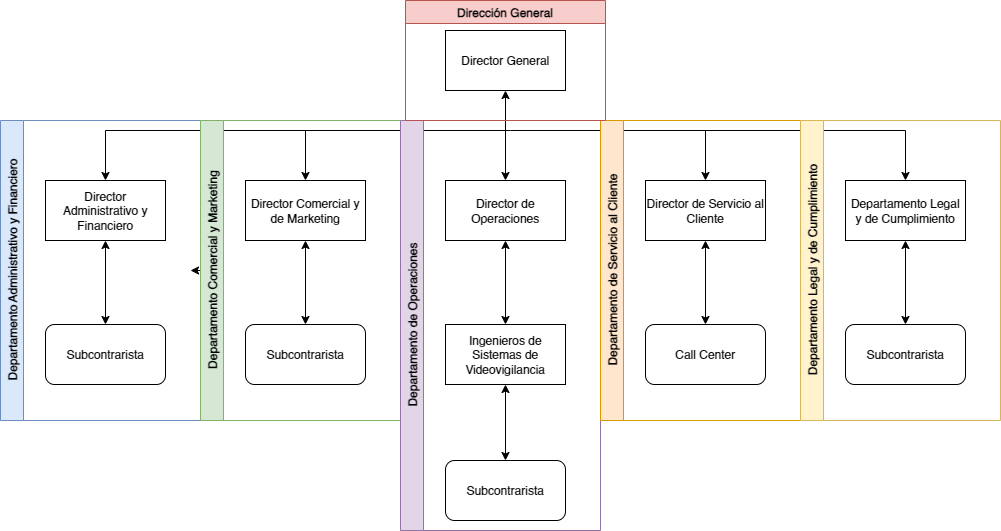
\includegraphics[width=1\textwidth]{./img/organigrama.png}
              \caption{Organigrama de SoloG}
            \end{figure}
          \clearpage\subsection{Costos de la estructura empresarial}
            \paragraph{}
            {
              La estructura empresarial de SoloG se resume en la siguiente tabla:
            }
            \begin{longtable}{|p{3cm}|p{3cm}|p{3cm}|p{3cm}|p{3cm}|}
              \hline
              \textbf{Departamentos} & \textbf{Puestos} & \textbf{Personal} & \textbf{Salario/anual} & \textbf{Costo total/anual}\\
              \hline
              \hline
              Dirección General & Director General & 1 & 100.000€ & 100.000€\\
              \hline
              Administración y Finanzas & Director Administrativo y Financiero & 1 & 80.000€ & 80.000€\\
              \hline
              Administración y Finanzas & Subcontratistas & 2 & 40.000€ & 80.000€\\
              \hline
              Comercial y Marketing & Director Comercial y de Marketing & 1 & 70.000€ & 70.000€\\
              \hline
              Comercial y Marketing & Subcontratistas & 2 & 35.000€ & 70.000€\\
              \hline
              Operaciones & Director de Operaciones & 1 & 60.000€ & 60.000€\\
              \hline
              Operaciones & Ingenieros de Sistemas de Videovigilancia & 3 & 40.000€ & 120.000€\\
              \hline
              Operaciones & Subcontratistas & 40 & 20.000€ & 800.000€\\
              \hline
              Servicio al Cliente & Director de Servicio al Cliente & 1 & 50.000€ & 50.000€\\
              \hline
              Servicio al Cliente & Call Center & 10 & 25.000€ & 250.000€\\
              \hline
              Legal y Cumplimiento & Director Legal y de Cumplimiento & 1 & 60.000€ & 60.000€\\
              \hline
              Legal y Cumplimiento & Subcontratistas & 2 & 30.000€ & 60.000€\\
              \hline
              \textbf{Total/anual}& - & 95 & - & 1.750.000€\\
              \hline
              \caption{Estructura empresarial de SoloG}
            \end{longtable}
        \clearpage\section{Infraestructuras}
          \paragraph*{}
          {
            Las infraestructuras son los activos físicos y tecnológicos que soportan las operaciones de una empresa. 
            Incluyen edificios, equipos, sistemas de información, redes de comunicación, software y hardware, entre otros.
          }
          \subsection{Desglose de la infraestructura}
            \paragraph*{}
            {
              Las infraestructuras de SoloG se dividen en diferentes categorías:
            }
            \subsubsection*{Infraestructura Física}
              \begin{itemize}
                \item Oficinas Corporativas - Espacio de oficinas para la dirección general, administración, ventas, operaciones, servicio al cliente y desarrollo tecnológico.
                \item Almacén y Centro de Distribución - Espacio de almacenamiento para equipos de videovigilancia, repuestos, suministros y productos terminados.
                \item Centro de Monitoreo - Sala de control para monitorear cámaras de seguridad, alarmas y sistemas de acceso en tiempo real.
                \item Laboratorio de Desarrollo - Espacio para la investigación y desarrollo de software y hardware especializado en videovigilancia.
              \end{itemize}
            \subsubsection*{Infraestructura Tecnológica}
              \begin{itemize}
                \item Red de Comunicación - Red de área local (LAN) y red de área amplia (WAN) para la comunicación interna y externa.
                \item Servidores y Almacenamiento - Servidores de aplicaciones, bases de datos y almacenamiento de datos para sistemas de videovigilancia.
              \end{itemize}
          \clearpage\subsection{Costes de la infraestructura}
            \begin{longtable}{|p{4cm}|p{4cm}|p{4cm}|p{4cm}|}
              \hline
              \textbf{Infraestructura} & \textbf{Costo de Adquisición} & \textbf{Costo de Mantenimiento} & \textbf{Costo Total/anual}\\
              \hline
              \hline
              Oficinas Corporativas & 500.000€ & 50.000€ & 550.000€\\
              \hline
              Almacén y Centro de Distribución & 300.000€ & 30.000€ & 330.000€\\
              \hline
              Centro de Monitoreo & 200.000€ & 20.000€ & 220.000€\\
              \hline
              Laboratorio de Desarrollo & 100.000€ & 10.000€ & 110.000€\\
              \hline
              Red de Comunicación & 50.000€ & 5.000€ & 55.000€\\
              \hline
              Servidores y Almacenamiento & 100.000€ & 10.000€ & 110.000€\\
              \hline
              \textbf{Total/anual} & - & - & 1.375.000€\\
              \hline
              \caption{Costos de la infraestructura de SoloG}
            \end{longtable}
        \clearpage\section{Productos}
          \subsection{Desglose de los Productos}
            \subsubsection*{Cámaras de Seguridad}
              \begin{itemize}
                \item Cámaras de CCTV (circuito cerrado de televisión) para interior y exterior.
                \item Cámaras domo, tipo bala, PTZ (pan-tilt-zoom) y de tipo discreto.
                \item Cámaras con tecnología de visión nocturna (infrarroja) para grabación en condiciones de poca luz.
                \item Cámaras con resolución de alta definición (HD) y ultra alta definición (4K) para imágenes claras y detalladas.
              \end{itemize}
            \subsubsection*{Sistemas de Grabación}
              \begin{itemize}
                \item Grabadoras de vídeo digital (DVR) y grabadoras de vídeo en red (NVR) para almacenamiento y gestión de grabaciones.
                \item Almacenamiento en disco duro con capacidades variables para retención de datos a largo plazo.
                \item Sistemas de almacenamiento en la nube para copias de seguridad y acceso remoto a grabaciones.
              \end{itemize}
            \subsubsection*{Sistemas de Control de Acceso}
              \begin{itemize}
                \item Lectores de tarjetas de acceso, teclados numéricos y sistemas biométricos de reconocimiento.
                \item Cerraduras electrónicas y electromagnéticas para control de puertas.
                \item Software de gestión de acceso para administrar usuarios, horarios y permisos de acceso.
              \end{itemize}
            \subsubsection*{Sistemas de Alarma}
              \begin{itemize}
                \item Sensores de movimiento, sensores de puertas y ventanas, y detectores de humo.
                \item Sirenas y luces estroboscópicas para disuadir intrusos y alertar a los ocupantes.
                \item Paneles de control centralizados para armar, desarmar y gestionar alarmas.
              \end{itemize}
          \clearpage\subsection{Costes de los Productos}
            \begin{longtable}{|p{4cm}|p{4cm}|p{2cm}|p{2cm}|p{2cm}|}
              \hline
              \textbf{Categoria} & \textbf{Producto} & \textbf{Costo de compra} & \textbf{Precio de Venta} & \textbf{Margen de Beneficio}\\
              \hline
              \hline
              Cámaras de Seguridad & Cámaras de CCTV & 100€/u & 125€/u & 25€/u\\
              \hline
              Cámaras de Seguridad & Cámaras domo & 150€/u & 225€/u & 75€/u\\
              \hline
              Cámaras de Seguridad & Cámaras PTZ & 200€/u & 300€/u & 100€/u\\
              \hline
              Cámaras de Seguridad & Cámaras de visión nocturna & 250€/u & 375€/u & 125€/u\\
              \hline
              Cámaras de Seguridad & Cámaras de alta definición & 300€/u & 450€/u & 150€/u\\
              \hline
              Sistemas de Grabación & DVR & 200€/u & 250€/u & 50€/u\\
              \hline
              Sistemas de Grabación & NVR & 300€/u & 375€/u & 75€/u\\
              \hline
              Sistemas de Grabación & Almacenamiento en la nube & 6000/mes & 18000€/mes & 12000€/mes\\
              \hline
              Sistemas de Control de Acceso & Lectores de tarjetas & 50€/u & 62.5€/u & 12.5€/u\\
              \hline
              Sistemas de Control de Acceso & Cerraduras electrónicas & 100€/u & 125€/u & 25€/u\\
              \hline
              Sistemas de Control de Acceso & Software de gestión & 5000€/mes & 15000€/mes & 10000€/mes\\
              \hline
              Sistemas de Alarma & Sensores de movimiento & 20€/u & 25€/u & 5€/u\\
              \hline
              Sistemas de Alarma & Sirenas y luces & 30€/u & 37.5€/u & 7.5€/u\\
              \hline
              Sistemas de Alarma & Paneles de control & 50€/u & 62.5€/u & 12.5€/u\\
              \hline
              Sistemas de Alarma & Software de analisis facial & 10000/mes & 30000€/mes & 20000€/mes\\
              \hline
              \caption{Costos de los productos de SoloG}
            \end{longtable}
        \clearpage\section{Servicios}
          \subsection{Desglose de los servicios}
            \subsubsection*{Consultoría en Seguridad}
              \begin{itemize}
                \item Evaluación de riesgos de seguridad y recomendaciones para mejorar la protección de las instalaciones.
                \item Desarrollo de planes de seguridad y políticas de gestión de riesgos.
              \end{itemize}
            \subsubsection*{Diseño e Instalación de Sistemas}
              \begin{itemize}
                \item Planificación y diseño de sistemas de videovigilancia personalizados según las necesidades y el entorno del cliente.
                \item Instalación profesional de equipos de seguridad, incluyendo cableado, montaje y configuración de dispositivos.
              \end{itemize}
            \subsubsection*{Mantenimiento Preventivo y Soporte Técnico}
              \begin{itemize}
                \item Programación de visitas periódicas para inspección y mantenimiento de equipos.
                \item Soporte técnico remoto y en sitio para resolver problemas y asegurar el funcionamiento continuo del sistema.
              \end{itemize}
            \subsubsection*{Capacitación y Formación}
              \begin{itemize}
                \item Entrenamiento para usuarios finales en el manejo y operación del sistema de videovigilancia.
                \item Capacitación técnica para personal de seguridad y administradores del sistema.
              \end{itemize}
            \subsubsection*{Servicios de Monitoreo y Respuesta a Alarmas}
              \begin{itemize}
                \item Monitoreo en tiempo real de cámaras y sistemas de seguridad por parte de personal capacitado.
                \item Respuesta a eventos de alarma, incluyendo notificación a las autoridades pertinentes según sea necesario.
              \end{itemize}
          \clearpage\subsection{Costes de los servicios}
            \paragraph*{}
            {
              Los costes, teniendo en cuenta los precios de la competencia y del sector en el que trabajamos, se resumen en la siguiente tabla:
            }
            \begin{longtable}{|p{5cm}|p{5cm}|p{5cm}|}
              \hline
              \textbf{Categoria} & \textbf{Servicio} & \textbf{Costo de Prestación}\\
              \hline
              \hline
              Consultoría en Seguridad & Evaluación de riesgos & 15000€/u\\
              \hline
              Consultoría en Seguridad & Desarrollo de planes de seguridad & 25000€/u\\
              \hline
              Diseño e Instalación de Sistemas & Planificación y diseño & 30000€/u\\
              \hline
              Diseño e Instalación de Sistemas & Instalación profesional & 40000€/u\\
              \hline
              Mantenimiento Preventivo y Soporte Técnico & Programación de visitas & 5000€/u\\
              \hline
              Mantenimiento Preventivo y Soporte Técnico & Soporte técnico remoto & 2000€/u\\
              \hline
              Capacitación y Formación & Entrenamiento para usuarios finales & 6000€/u\\
              \hline
              Capacitación y Formación & Capacitación técnica & 10000€/u\\
              \hline
              Servicios de Monitoreo y Respuesta a Alarmas & Monitoreo en tiempo real & 20000€/mes\\
              \hline
              Servicios de Monitoreo y Respuesta a Alarmas & Respuesta a eventos de alarma & 10000€/mes\\
              \hline
              \caption{Costos de los servicios de SoloG}
            \end{longtable}
    \chapter{Diseño del sistema de gestión}
      \paragraph*{}
      {
        El sistema de gestión de SoloG es un conjunto de procesos, procedimientos y herramientas que se utilizan para planificar, organizar, dirigir y controlar las actividades de la empresa. 
        El objetivo del sistema de gestión es mejorar la eficiencia, la efectividad y la calidad de los productos y servicios de la empresa, así como garantizar el cumplimiento de los objetivos organizacionales.
        Para ello, se han definido los siguientes elementos del sistema de gestión:
      }
      \section{Procesos}
        {
          Los procesos son las actividades y tareas que se realizan en una empresa para lograr los objetivos organizacionales. 
          Son esenciales para la operación eficiente y efectiva de una empresa, ya que definen cómo se llevan a cabo las actividades, cómo se asignan los recursos y cómo se logran los resultados.
        }
        \paragraph*{}
        {
          Los procesos de SoloG se pueden clasificar en diferentes categorías:
        }
        \subsubsection*{Procesos de Ventas y Marketing}
          \begin{itemize}
            \item Identificación de Clientes Potenciales - Identificar empresas y organizaciones que puedan necesitar sistemas de videovigilancia.
            \item Desarrollo de Estrategias de Ventas - Crear estrategias de ventas personalizadas para cada cliente potencial.
            \item Negociación de Contratos - Negociar los términos y condiciones de los contratos con los clientes.
            \item Cierre de Ventas - Cerrar acuerdos de venta y asegurar la satisfacción del cliente.
            \item Desarrollo de Estrategias de Marketing - Crear campañas de marketing para promocionar los productos y servicios de la empresa.
            \item Publicidad y Promoción - Publicar anuncios en línea, en medios impresos y en eventos para promocionar la empresa.
            \item Relaciones Públicas - Mantener relaciones positivas con los medios de comunicación, clientes y la comunidad.
          \end{itemize}
        \subsubsection*{Procesos de Diseño y Consultoria}
          \begin{itemize}
            \item Diseño de Sistemas de Videovigilancia - Diseñar sistemas de videovigilancia personalizados para las necesidades de cada cliente.
            \item Consultoría en Seguridad - Asesorar a los clientes sobre las mejores prácticas de seguridad y las soluciones más efectivas.
            \item Evaluación de Riesgos - Evaluar los riesgos de seguridad de las instalaciones de los clientes y recomendar soluciones.
            \item Implementación de Sistemas de Seguridad - Instalar y configurar sistemas de videovigilancia en las instalaciones de los clientes.
            \item Capacitación de Personal - Capacitar al personal de los clientes en el uso de los sistemas de videovigilancia.
          \end{itemize}
        \subsubsection*{Procesos de Instalación y Mantenimiento}
          \begin{itemize}
            \item Instalación de Equipos de Videovigilancia - Instalar cámaras, grabadores de video y otros equipos de videovigilancia en las instalaciones de los clientes.
            \item Configuración de Sistemas de Seguridad - Configurar los sistemas de videovigilancia para garantizar su funcionamiento óptimo.
            \item Mantenimiento Preventivo - Realizar inspecciones regulares y mantenimiento preventivo de los sistemas de videovigilancia.
            \item Reparación de Equipos - Reparar equipos de videovigilancia dañados o defectuosos.
            \item Actualización de Software y Firmware - Actualizar el software y firmware de los sistemas de videovigilancia para garantizar su seguridad y eficacia.
          \end{itemize}
        \subsubsection*{Procesos de Servicio al Cliente}
          \begin{itemize}
            \item Atención de Consultas - Atender consultas de los clientes sobre productos, servicios y precios.
            \item Soporte Técnico - Proporcionar asistencia técnica a los clientes para resolver problemas con los sistemas de videovigilancia.
            \item Asistencia Postventa - Brindar asistencia a los clientes después de la venta para garantizar su satisfacción.
            \item Resolución de Quejas y Problemas - Resolver quejas y problemas de los clientes de manera rápida y eficaz.
            \item Mantenimiento de Relaciones con Clientes - Mantener relaciones positivas con los clientes para fomentar la lealtad y la satisfacción.
          \end{itemize}
        \subsubsection*{Procesos de Investigación y Desarrollo}
          \begin{itemize}
            \item Investigación de Nuevas Tecnologías - Investigar y evaluar nuevas tecnologías en videovigilancia para mejorar los productos y servicios de la empresa.
            \item Desarrollo de Software de Videovigilancia - Desarrollar software especializado para la gestión y análisis de sistemas de videovigilancia.
            \item Desarrollo de Hardware Especializado - Diseñar y fabricar hardware especializado para sistemas de videovigilancia.
            \item Pruebas y Validación de Productos - Realizar pruebas exhaustivas y validación de productos antes de su lanzamiento al mercado.
            \item Implementación de Mejoras - Implementar mejoras continuas en los productos y servicios de la empresa para mantenerse a la vanguardia de la tecnología.
          \end{itemize}
      \clearpage\section{Diagramas de procesos}
        \subsection*{Procesos de Ventas y Marketing}
          \begin{figure}[H]
            \centering
            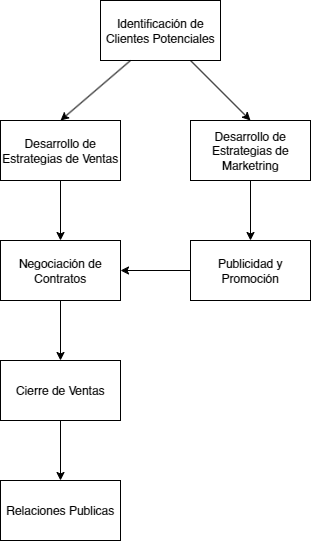
\includegraphics[width=0.6\textwidth]{./img/pro_ven_mark.png}
            \caption{Diagrama de procesos de Ventas y Marketing}
          \end{figure}
        \clearpage\subsection*{Procesos de Diseño e Instalación}
          \begin{figure}[H]
            \centering
            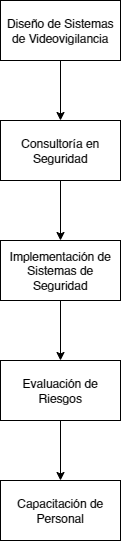
\includegraphics[width=0.2\textwidth]{./img/pro_dis_con.png}
            \caption{Diagrama de procesos de Diseño e Instalación}
          \end{figure}
        \clearpage\subsection*{Procesos de Mantenimiento y Soporte}
          \begin{figure}[H]
            \centering
            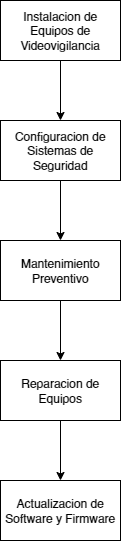
\includegraphics[width=0.2\textwidth]{./img/pro_int_mant.png}
            \caption{Diagrama de procesos de Mantenimiento y Soporte}
          \end{figure}
        \clearpage\subsection*{Procesos de Servicio al Cliente}
          \begin{figure}[H]
            \centering
            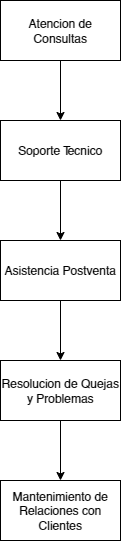
\includegraphics[width=0.2\textwidth]{./img/pro_ser_cli.png}
            \caption{Diagrama de procesos de Servicio al Cliente}
          \end{figure}
        \clearpage\subsection*{Procesos de Investigación y Desarrollo}
          \begin{figure}[H]
            \centering
            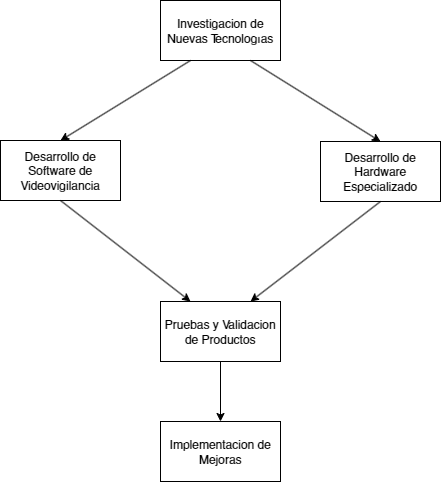
\includegraphics[width=0.8\textwidth]{./img/pro_inv_des.png}
            \caption{Diagrama de procesos de Investigación y Desarrollo}
          \end{figure}
      \clearpage\section{Modulos de Odoo}
        \begin{longtable}{|p{3cm}|p{3cm}|p{7cm}|}
          \hline
          \textbf{Módulo} & \textbf{Descripción} & \textbf{Funcionalidades}\\
          \hline
          \hline
          CRM & Gestión de relaciones con clientes & Oportunidades, clientes, contactos, actividades\\
          \hline
          Ventas & Gestión de ventas & Presupuestos, pedidos, facturas, tarifas de precios, descuentos\\
          \hline
          Tableros & Tableros de control & Informes, gráficos, indicadores clave de rendimiento\\
          \hline
          Proyectos & Gestión de proyectos & Proyectos, tareas, etapas, responsables, seguimiento\\
          \hline
          Sitio web & Gestión de sitio web & Páginas, productos, blog, foro, chat en vivo\\
          \hline
          Compras & Gestión de compras & Órdenes de compra, proveedores, tarifas de precios, descuentos\\
          \hline
          Inventario & Gestión de inventario & Productos, almacenes, ubicaciones, movimientos, inventarios físicos\\
          \hline
          Fabricación & Gestión de fabricación & Órdenes de fabricación, lista de materiales, costes, tiempos\\
          \hline
          Empleados & Gestión de recursos humanos & Empleados, departamentos, permisos, nóminas\\
          \hline
          \caption{Módulos de Odoo para el sistema de gestión de SoloG}
        \end{longtable}
    \chapter{Presentación de los resultados}
        \section*{Ventas}
            \begin{figure}[H]
                \centering
                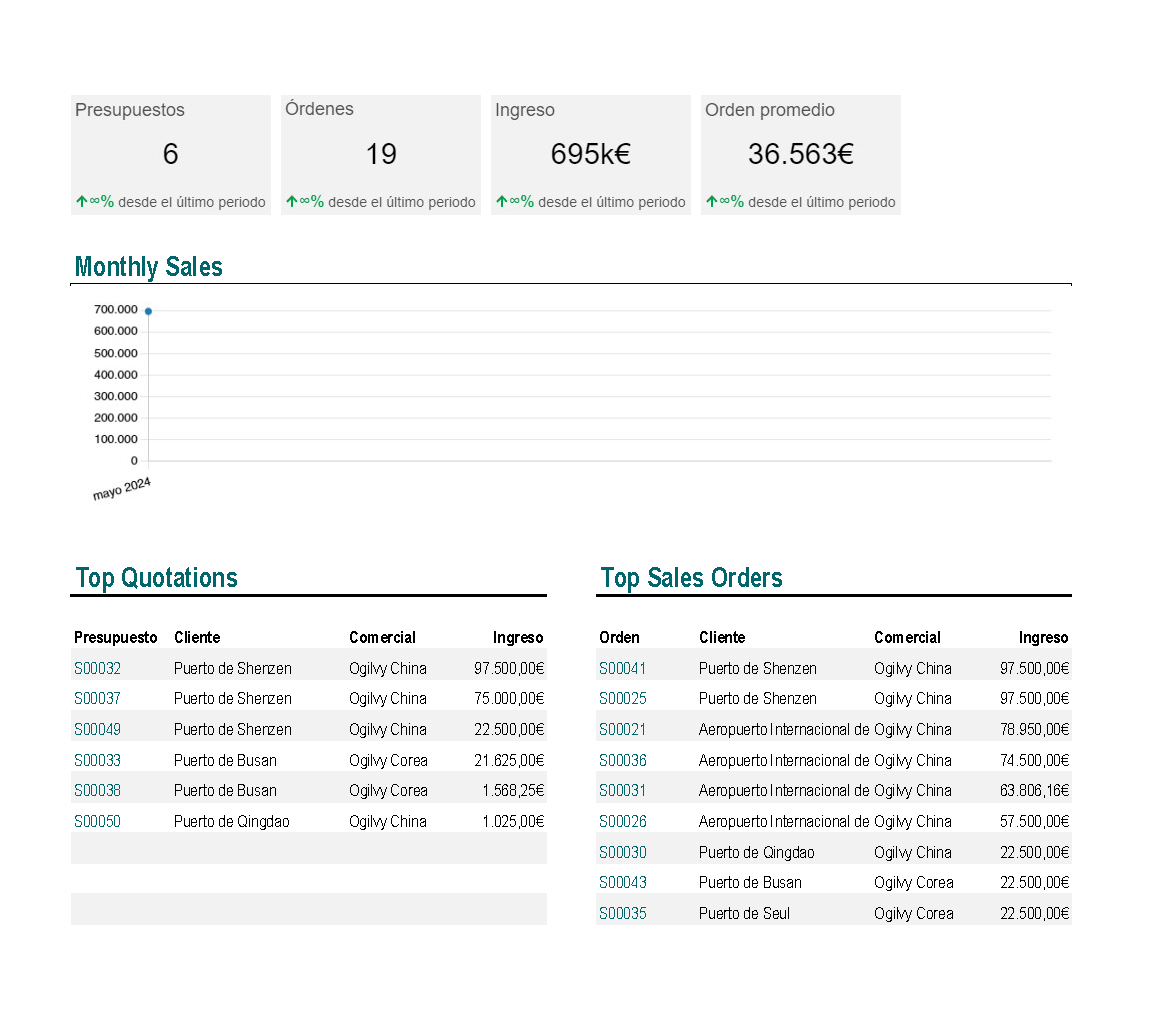
\includegraphics[width=0.55\textwidth]{./img/Ventas1.png}
                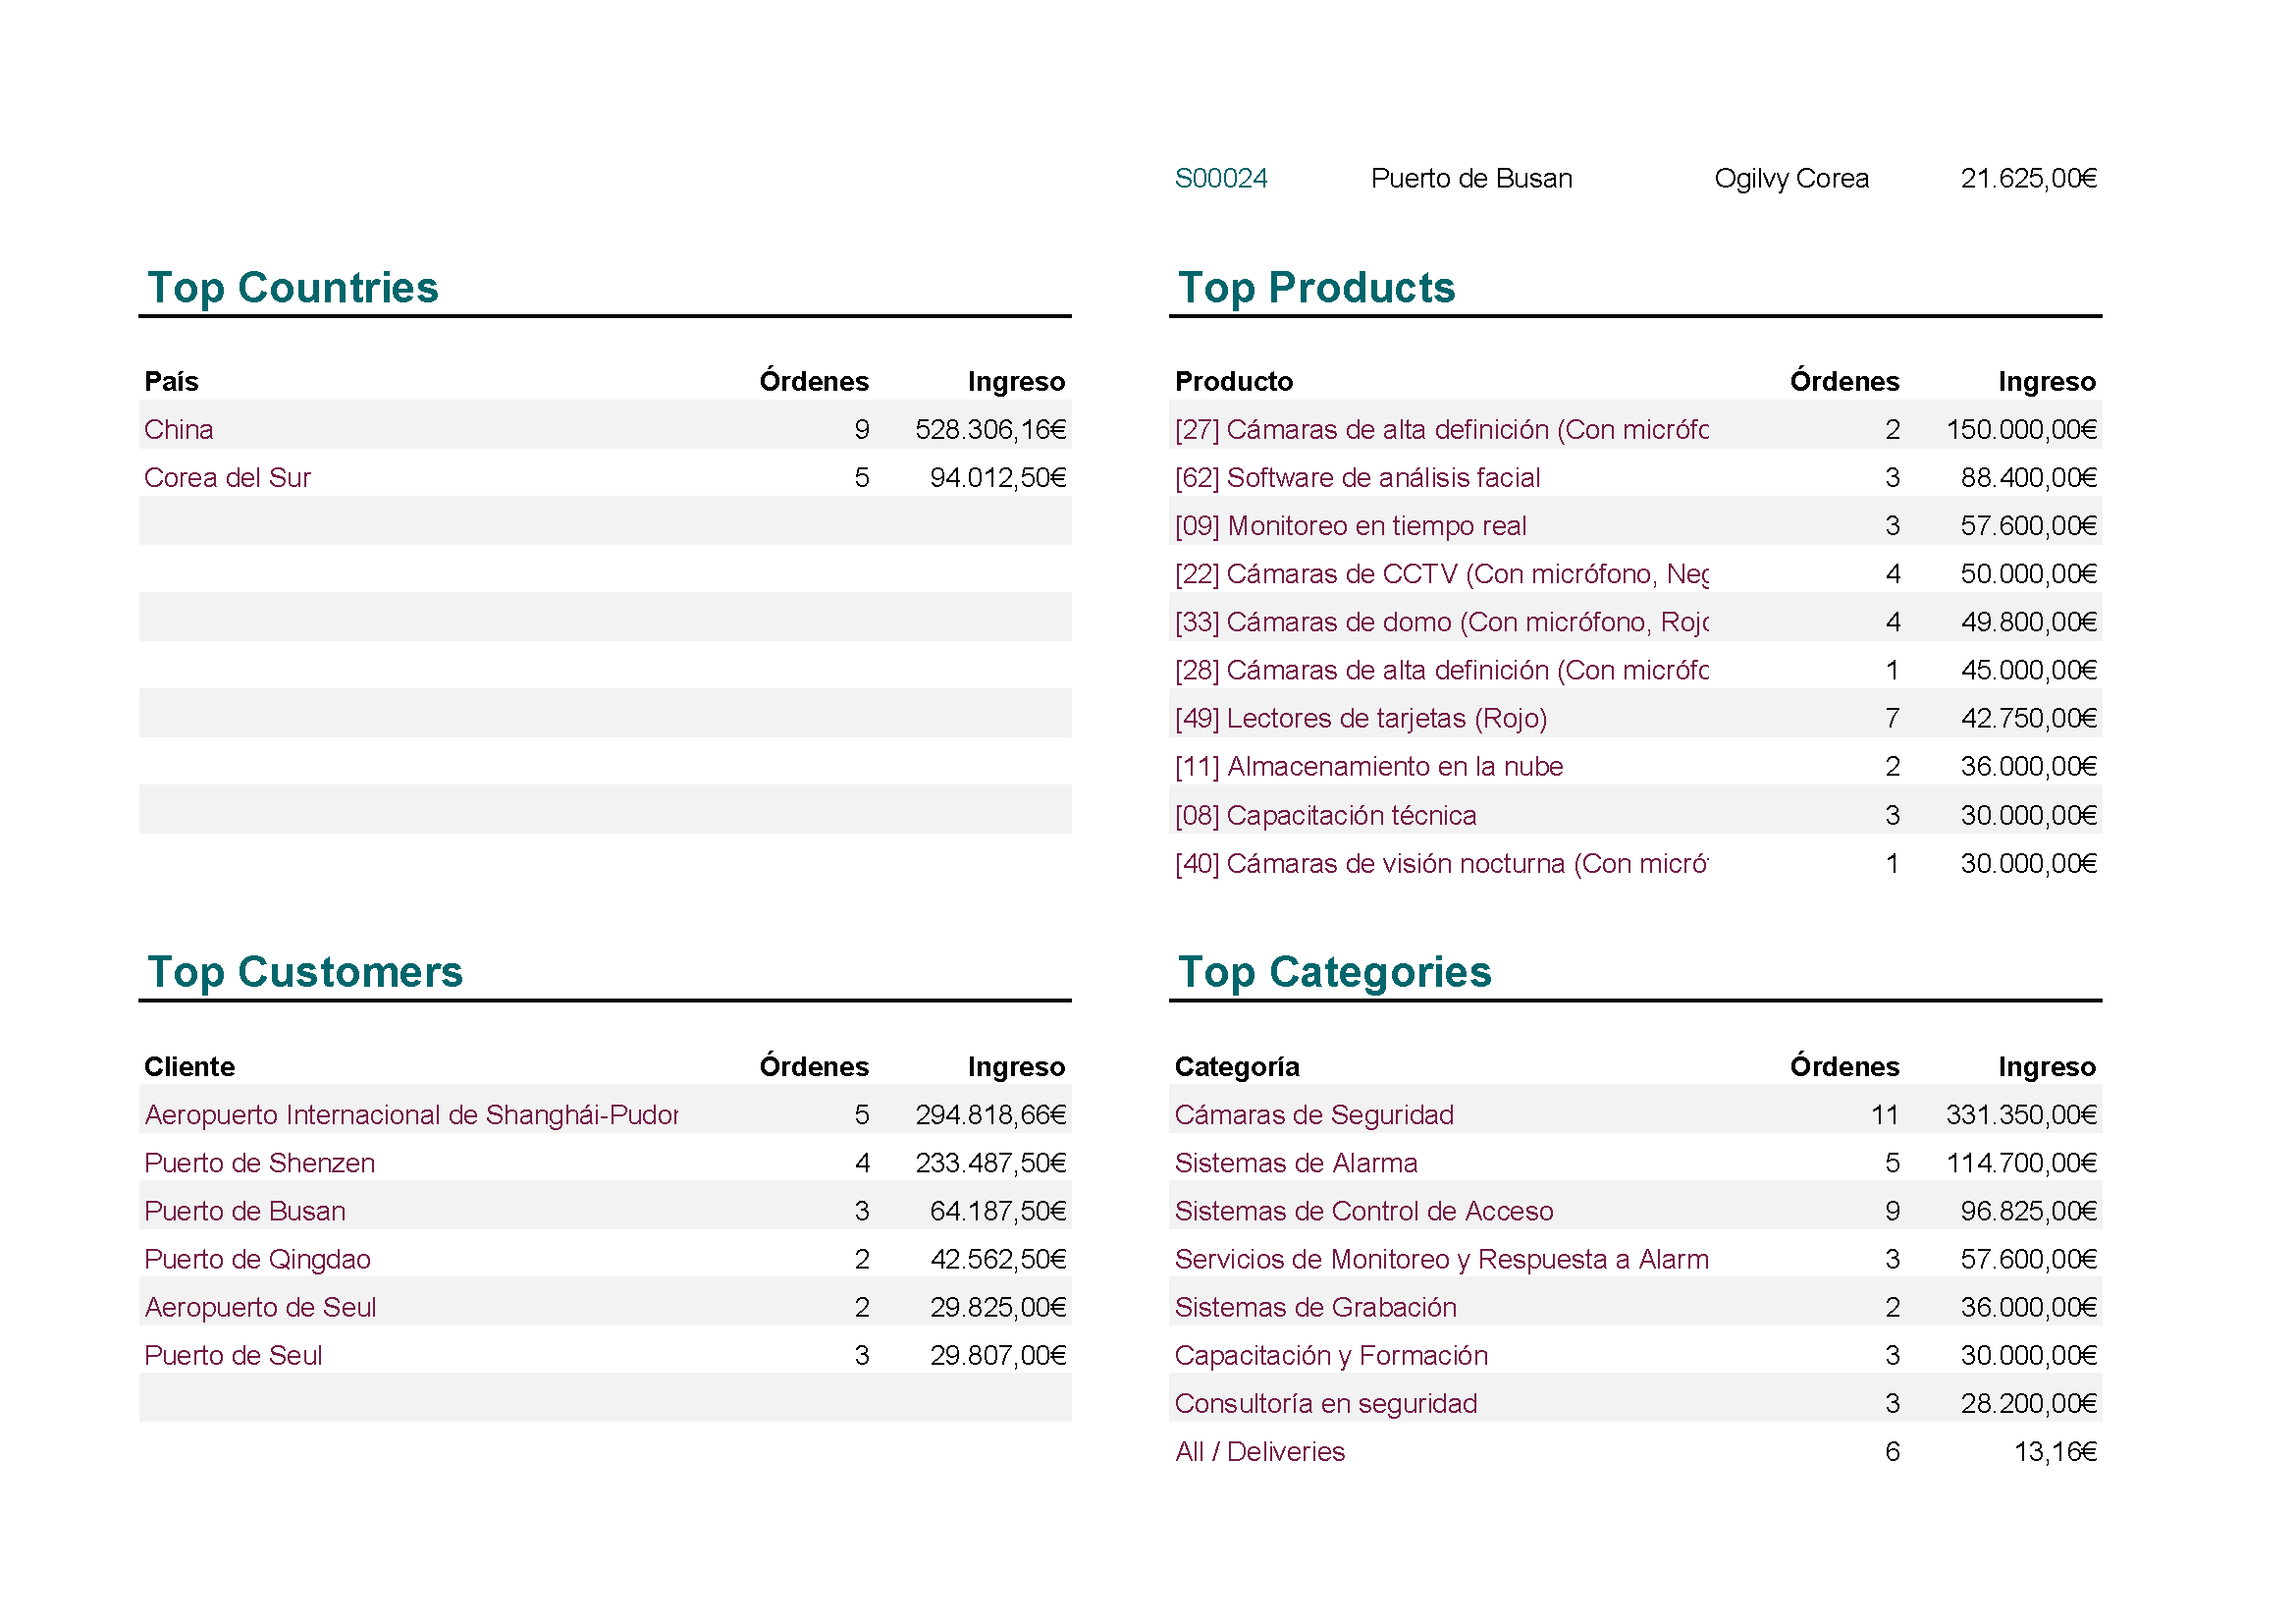
\includegraphics[width=0.55\textwidth]{./img/Ventas2.png}
                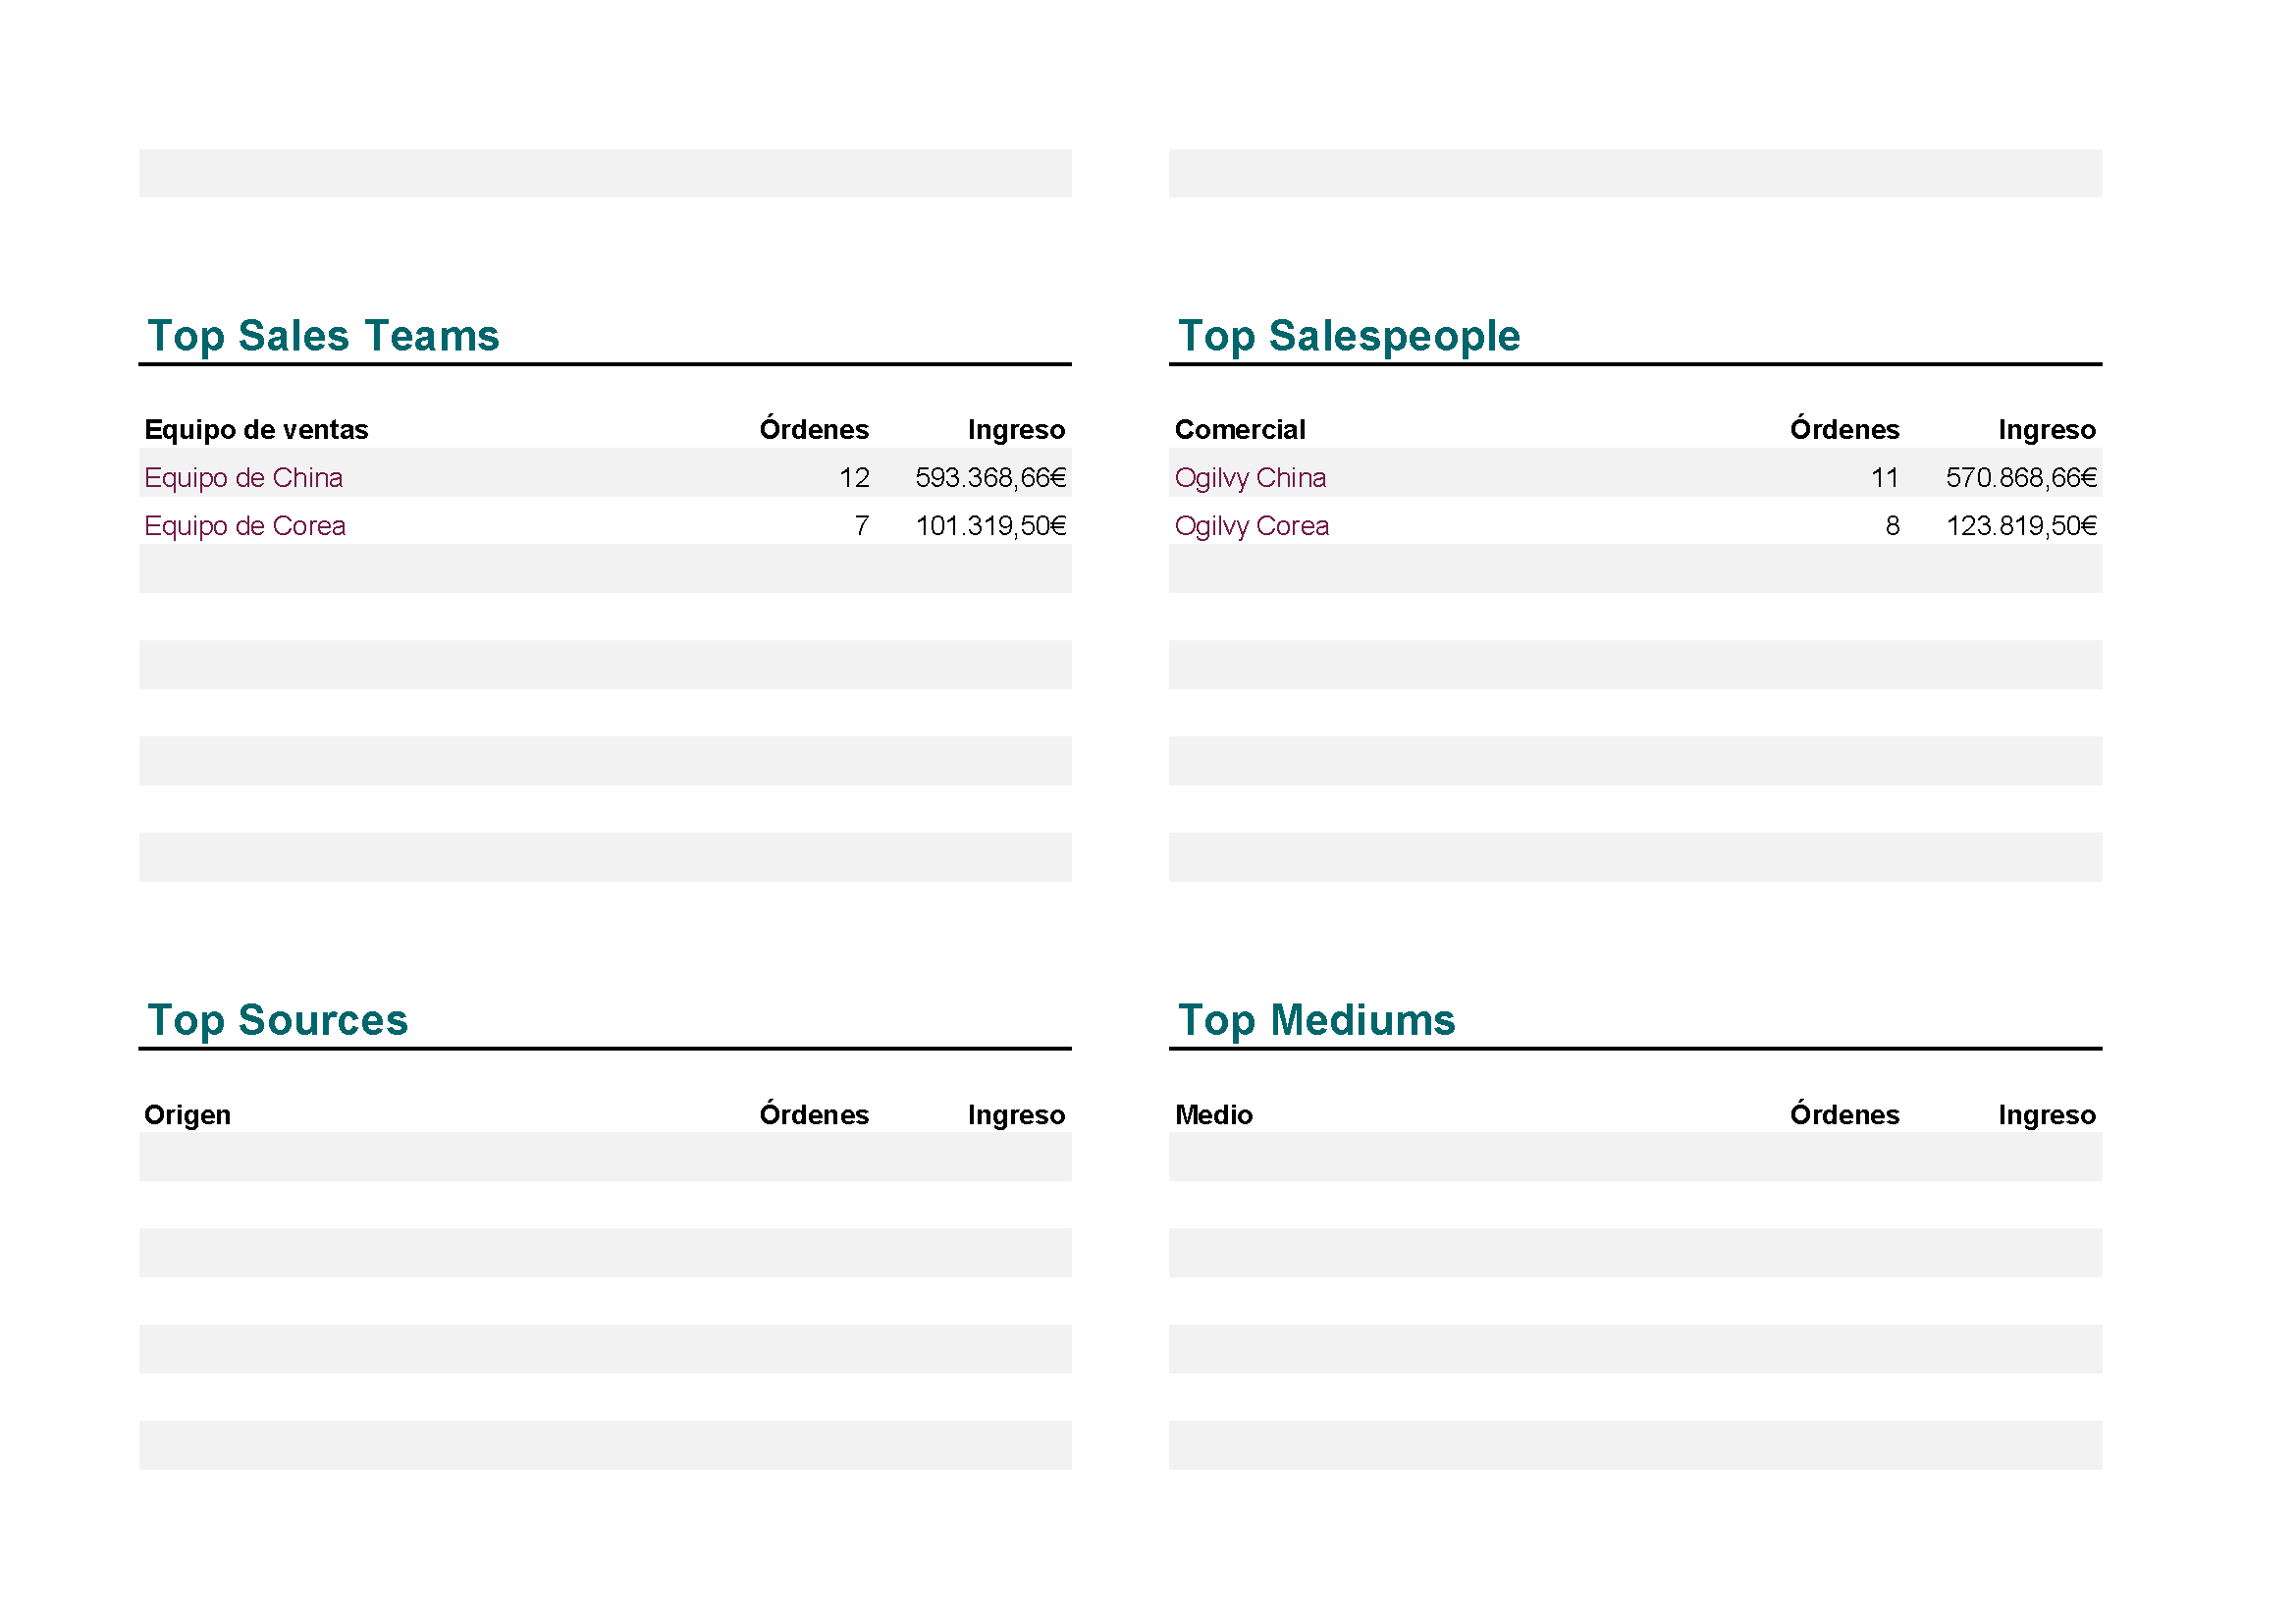
\includegraphics[width=0.55\textwidth]{./img/Ventas3.png}
                \caption{Resultados de las ventas}
            \end{figure}
        \section*{Productos}
            \begin{figure}[H]
                \centering
                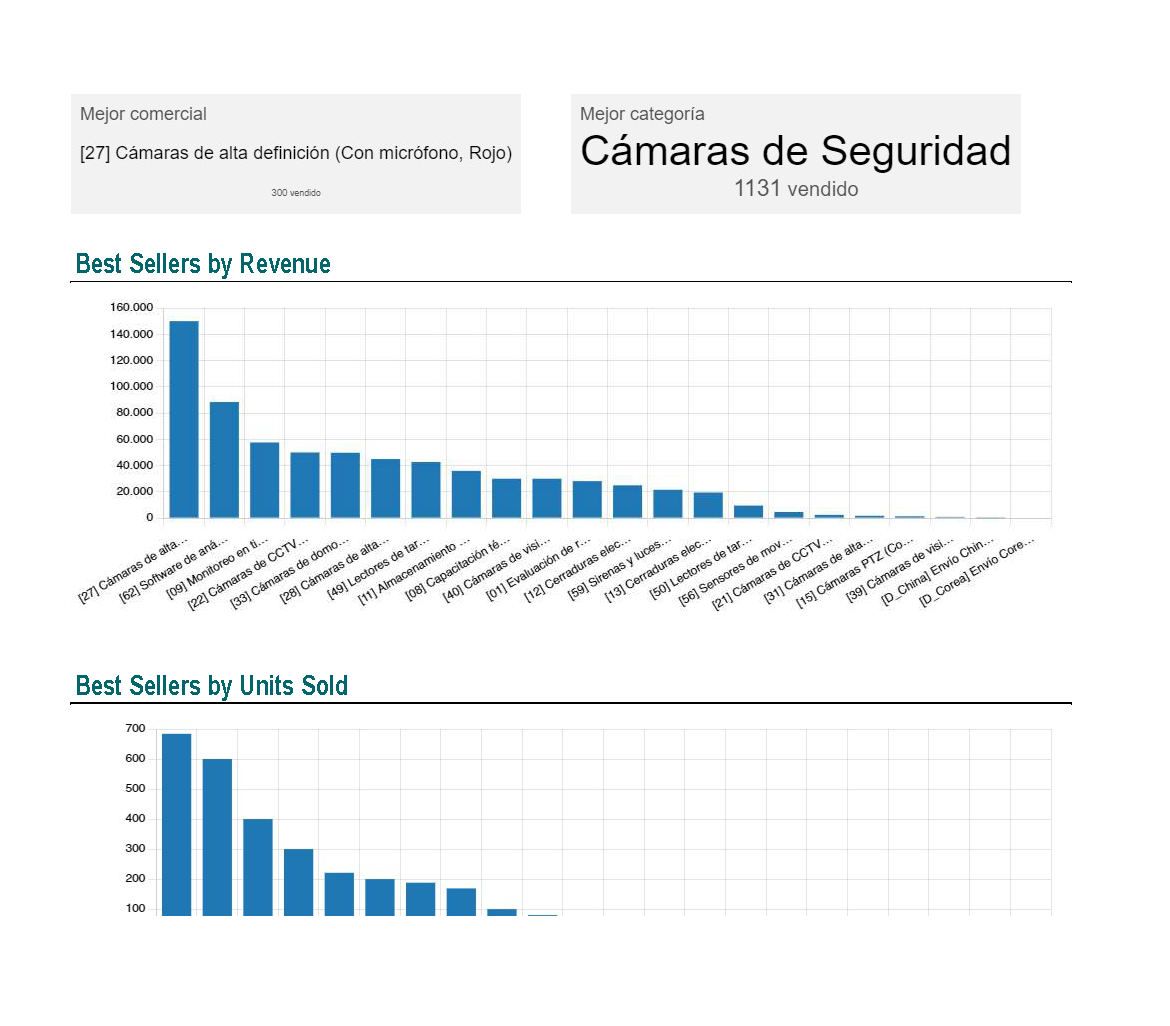
\includegraphics[width=0.8\textwidth]{./img/Producto1.png}
                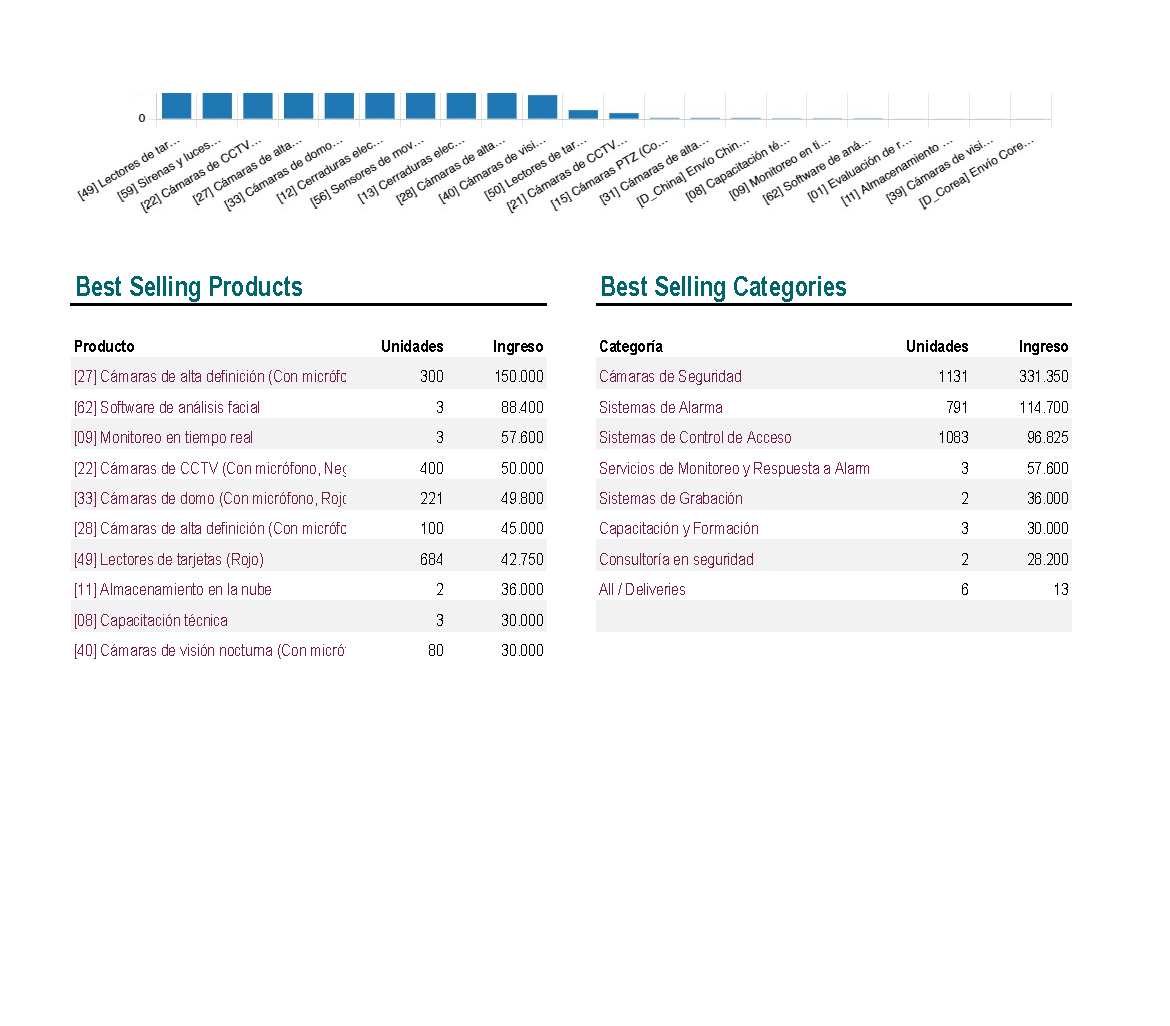
\includegraphics[width=0.8\textwidth]{./img/Producto2.png}
                \caption{Resultados de los productos}
            \end{figure}
        \section*{Leads}
            \begin{figure}[H]
                \centering
                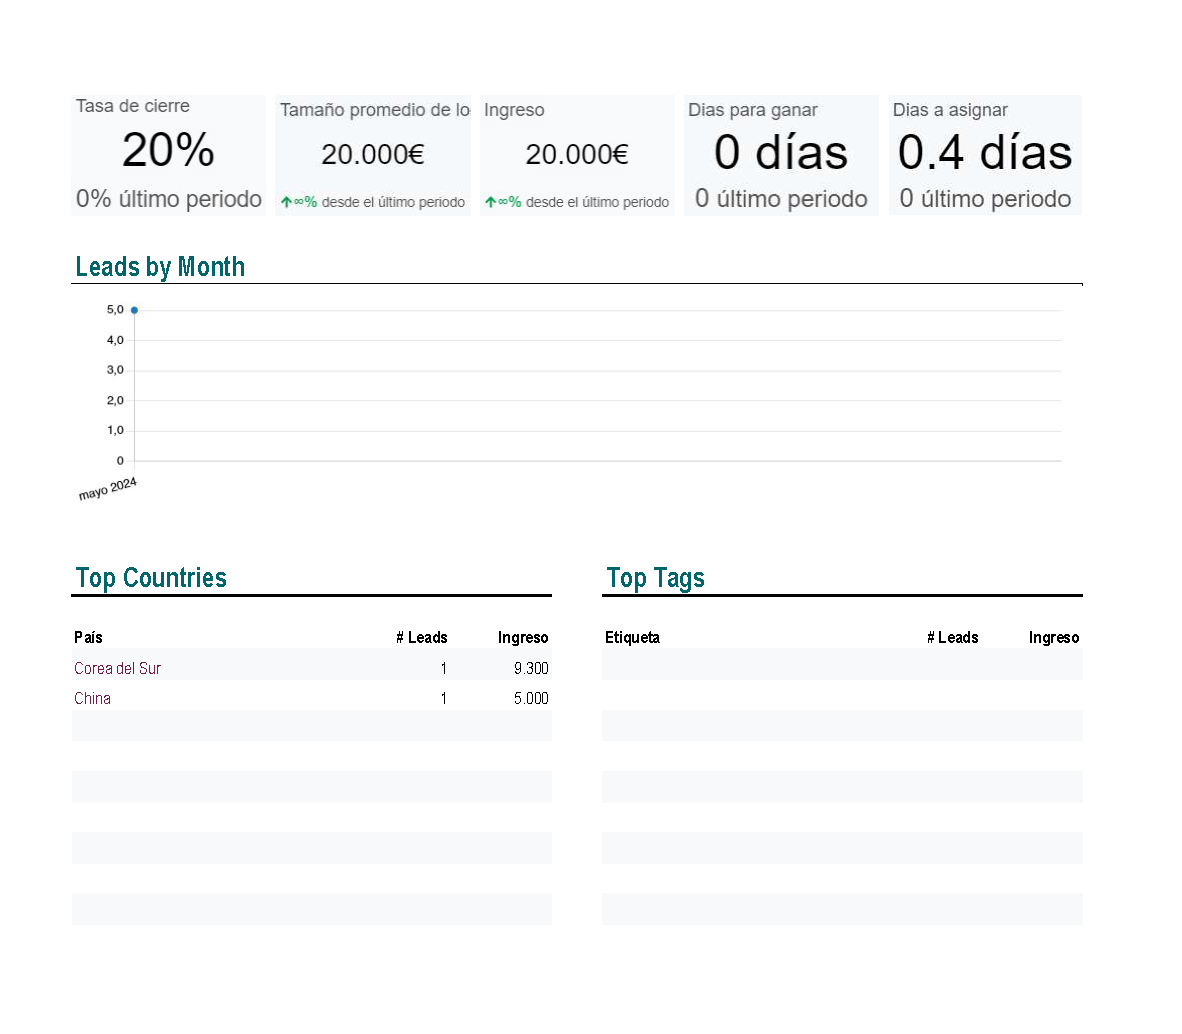
\includegraphics[width=0.8\textwidth]{./img/Leads1.png}
                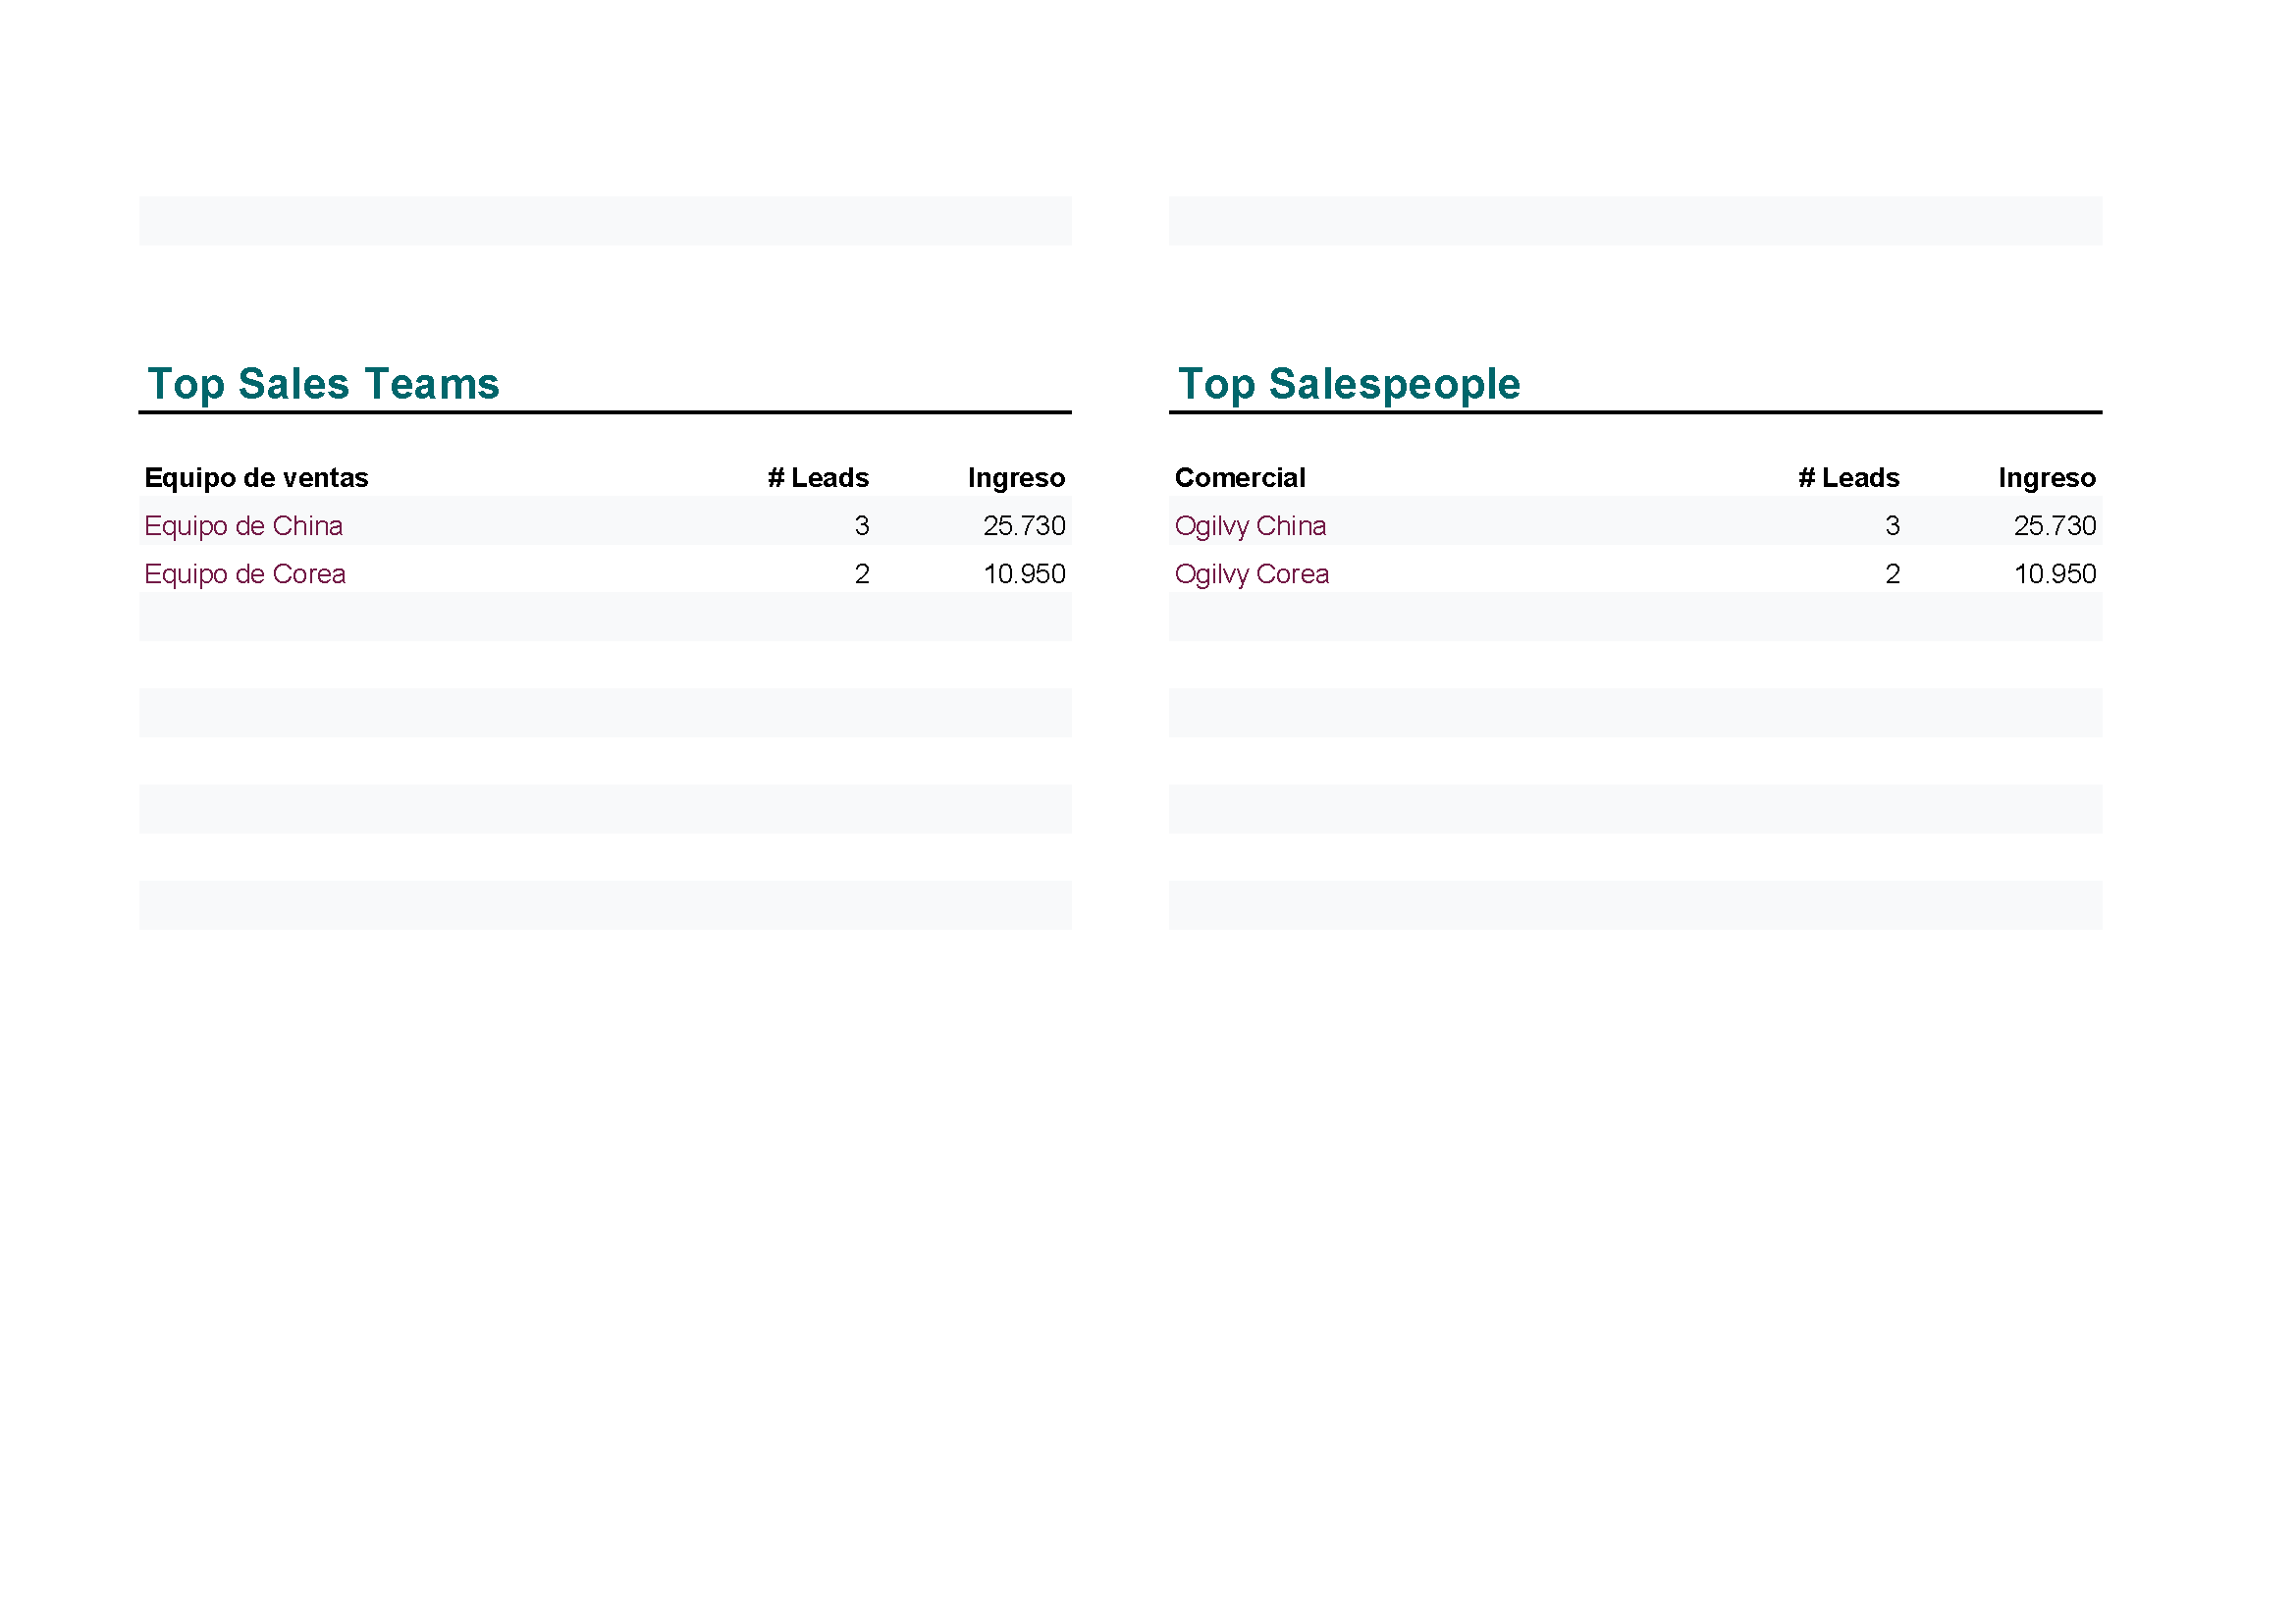
\includegraphics[width=0.8\textwidth]{./img/Leads2.png}
                \caption{Resultado de los Leads del CRM}
            \end{figure}
        \section*{Pipeline}
            \begin{figure}[H]
                \centering
                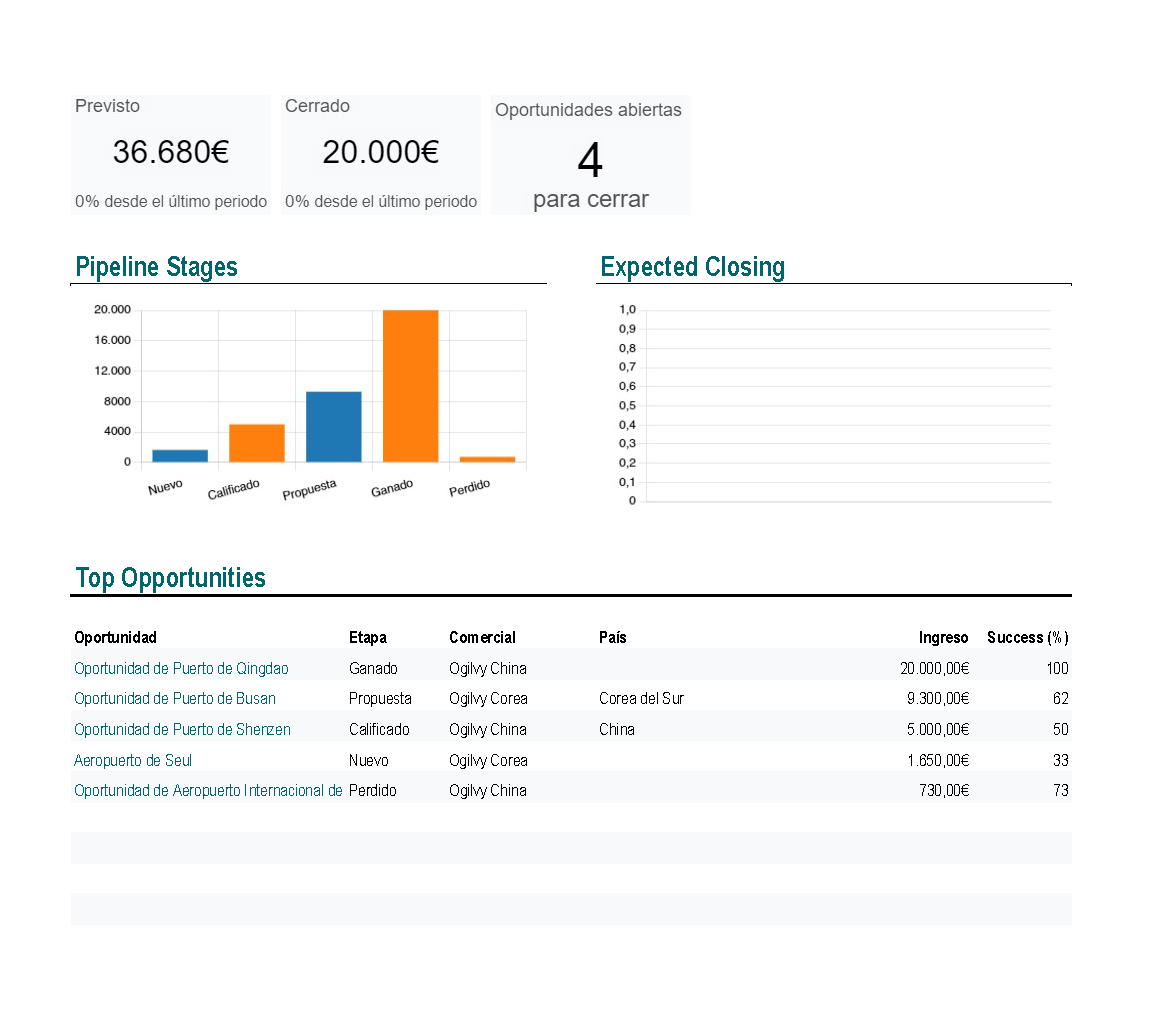
\includegraphics[width=0.8\textwidth]{./img/Pipeline1.png}
                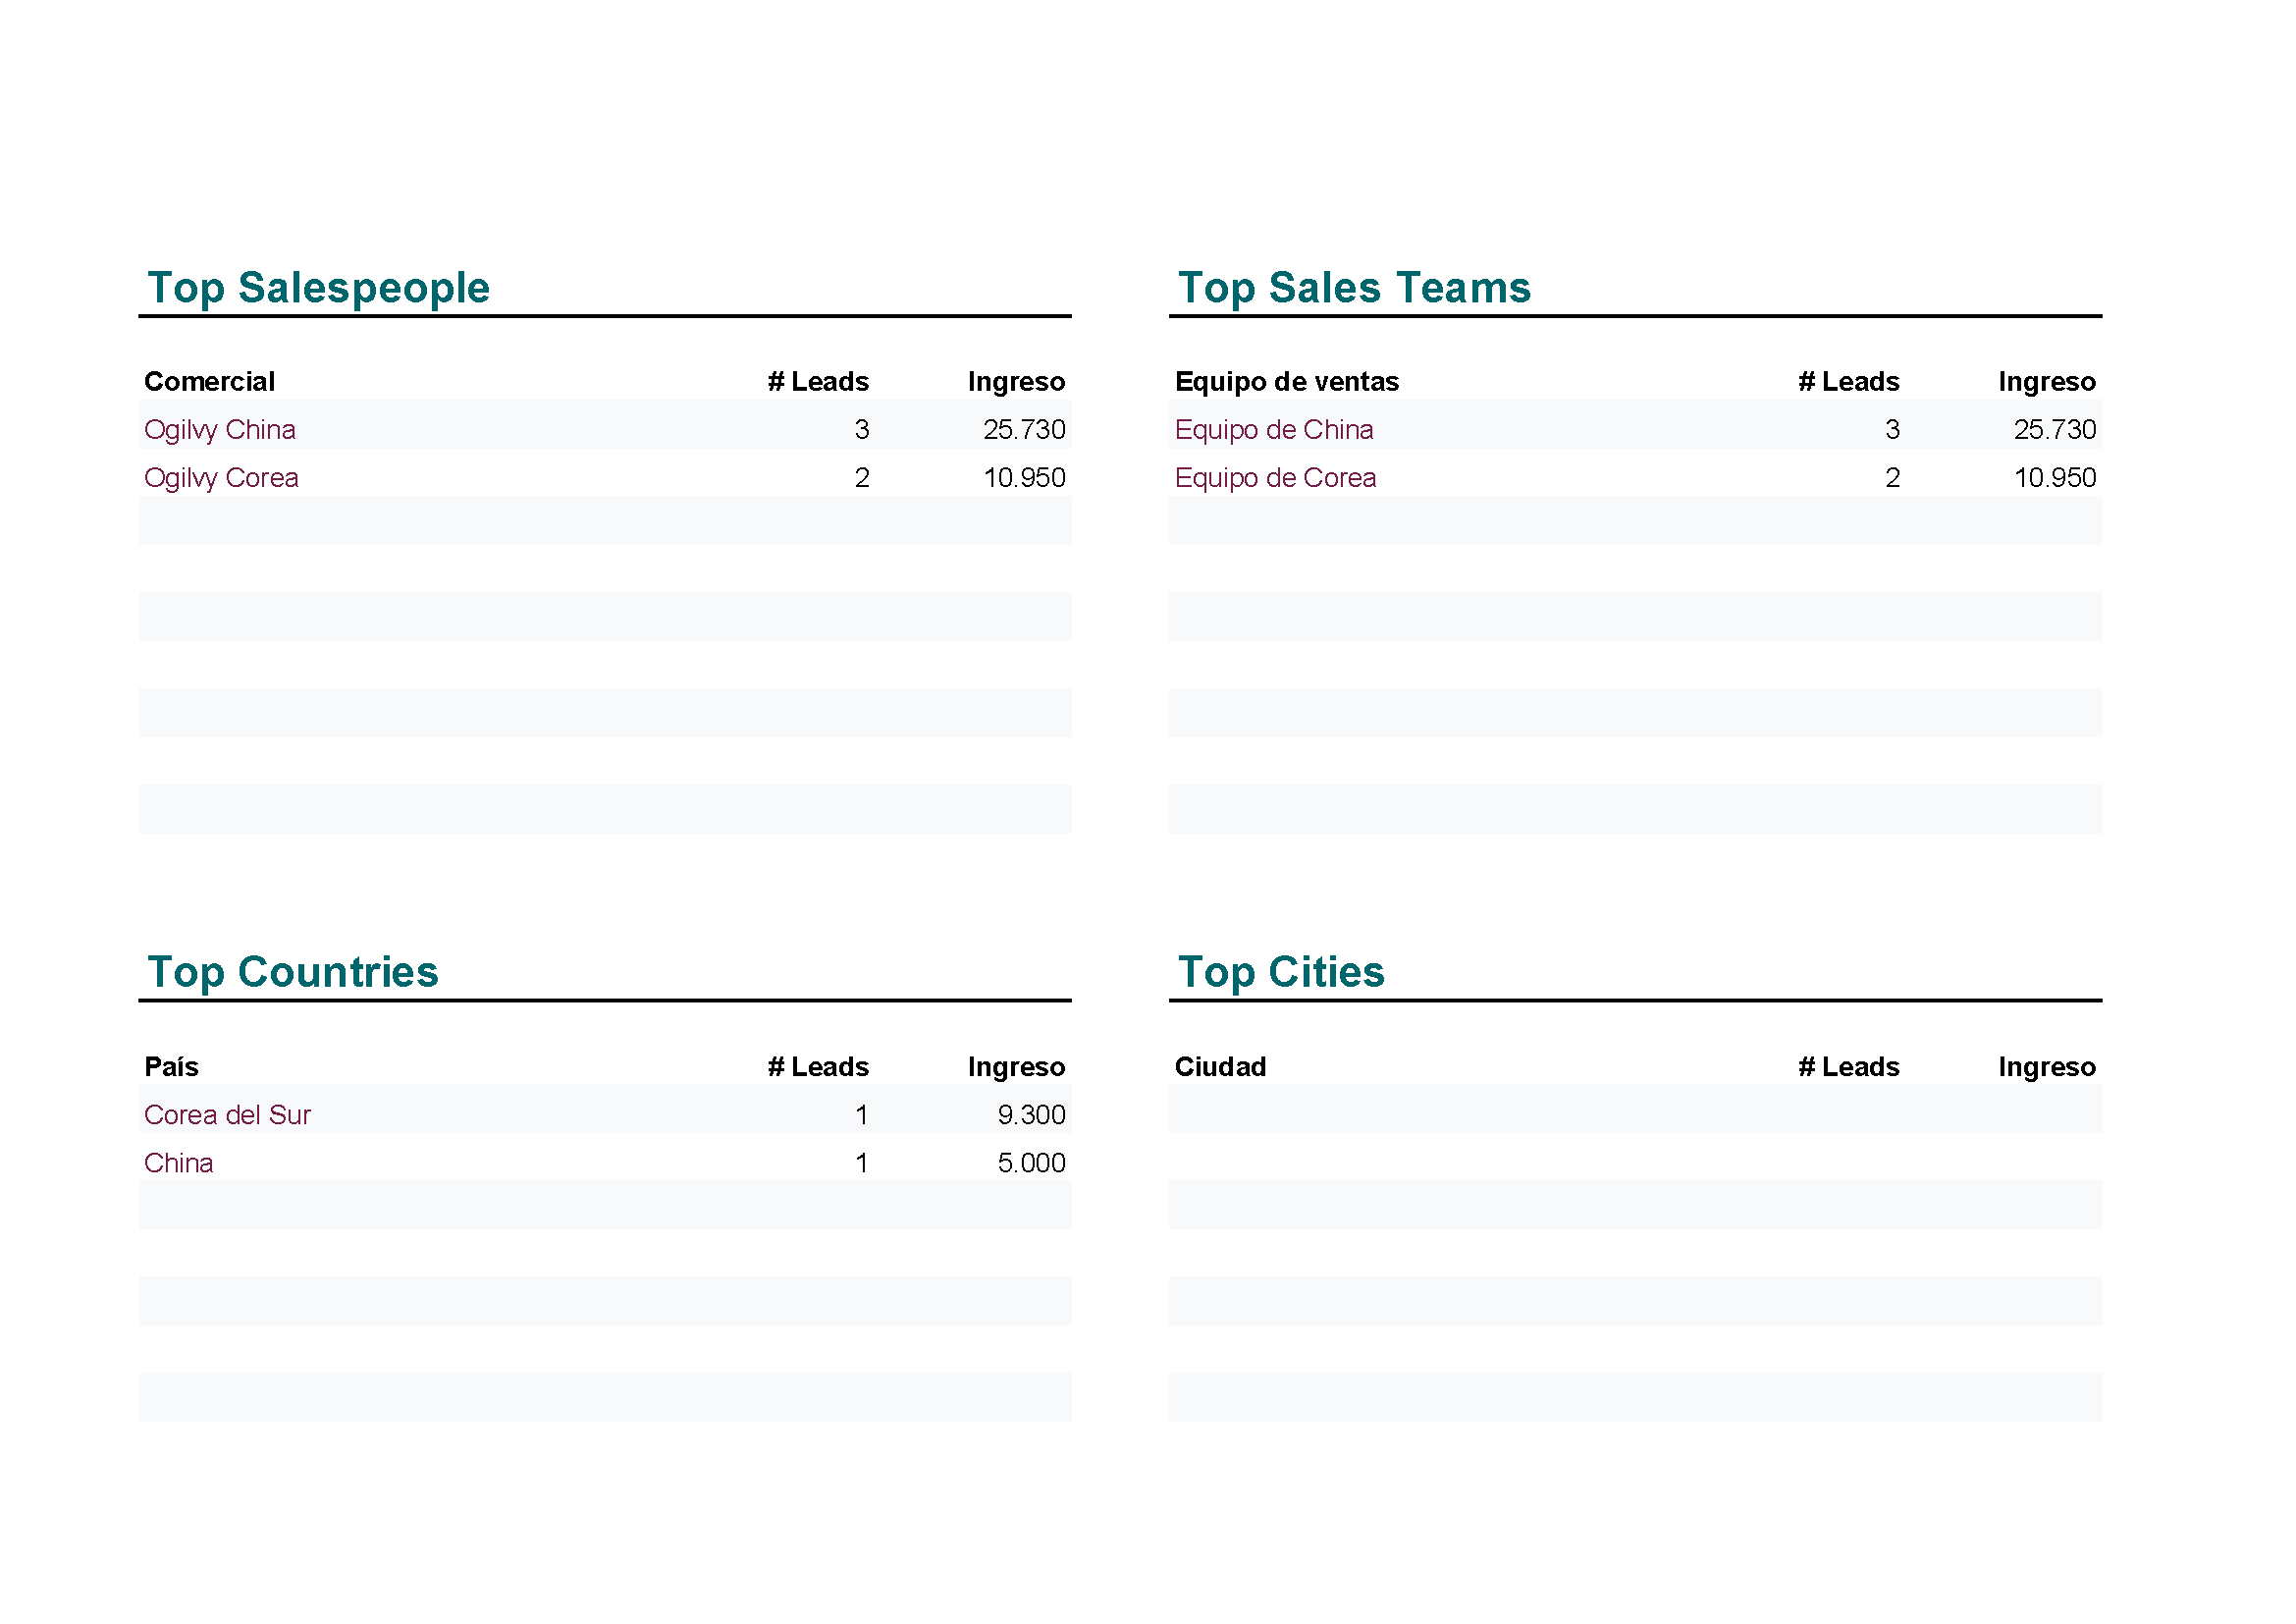
\includegraphics[width=0.8\textwidth]{./img/Pipeline2.png}
                \caption{Resultados de las Pipeline del CRM}
            \end{figure}
        \section*{Contabilidad}
            \begin{figure}[H]
                \centering
                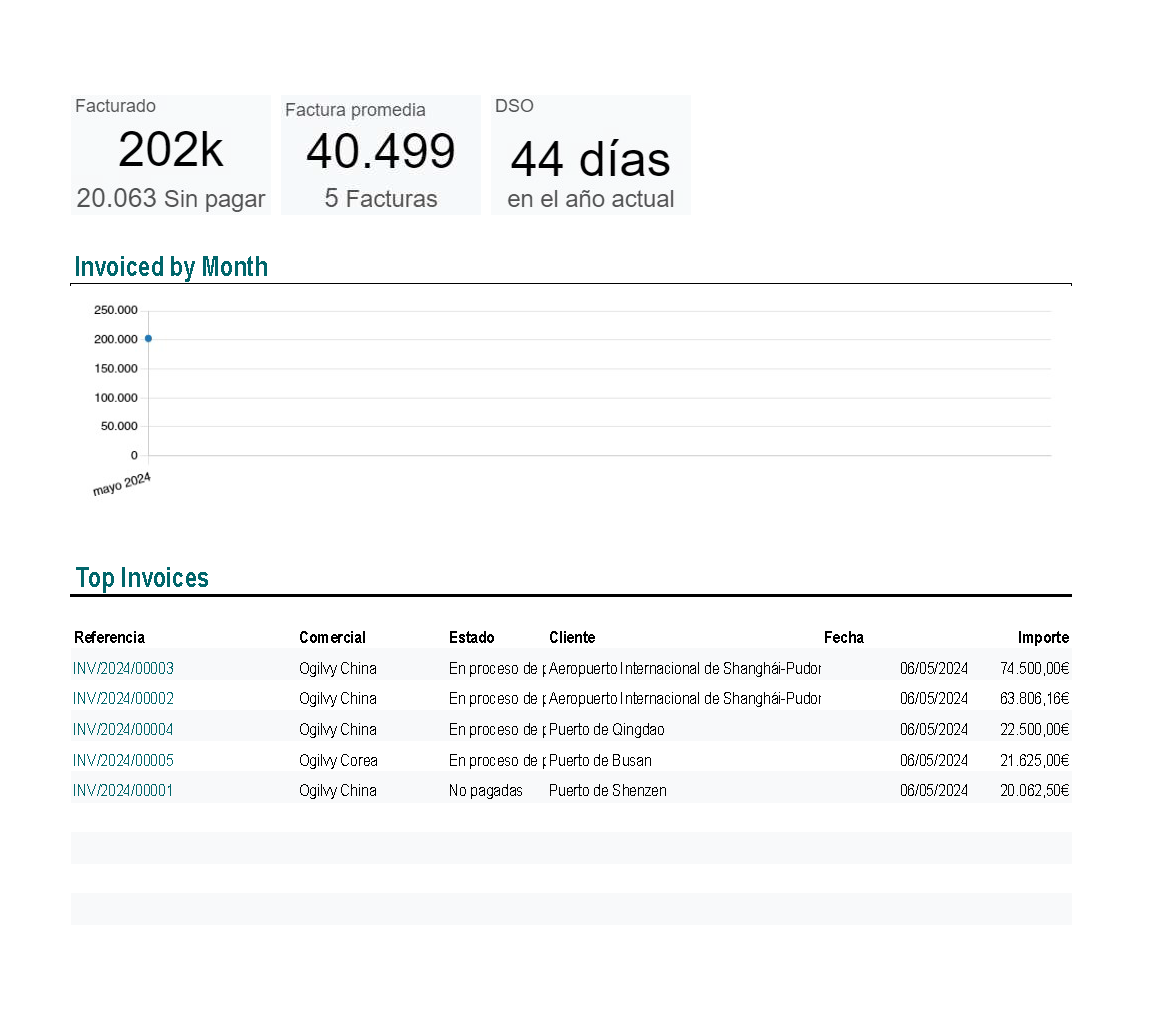
\includegraphics[width=0.8\textwidth]{./img/Contabilidad1.png}
                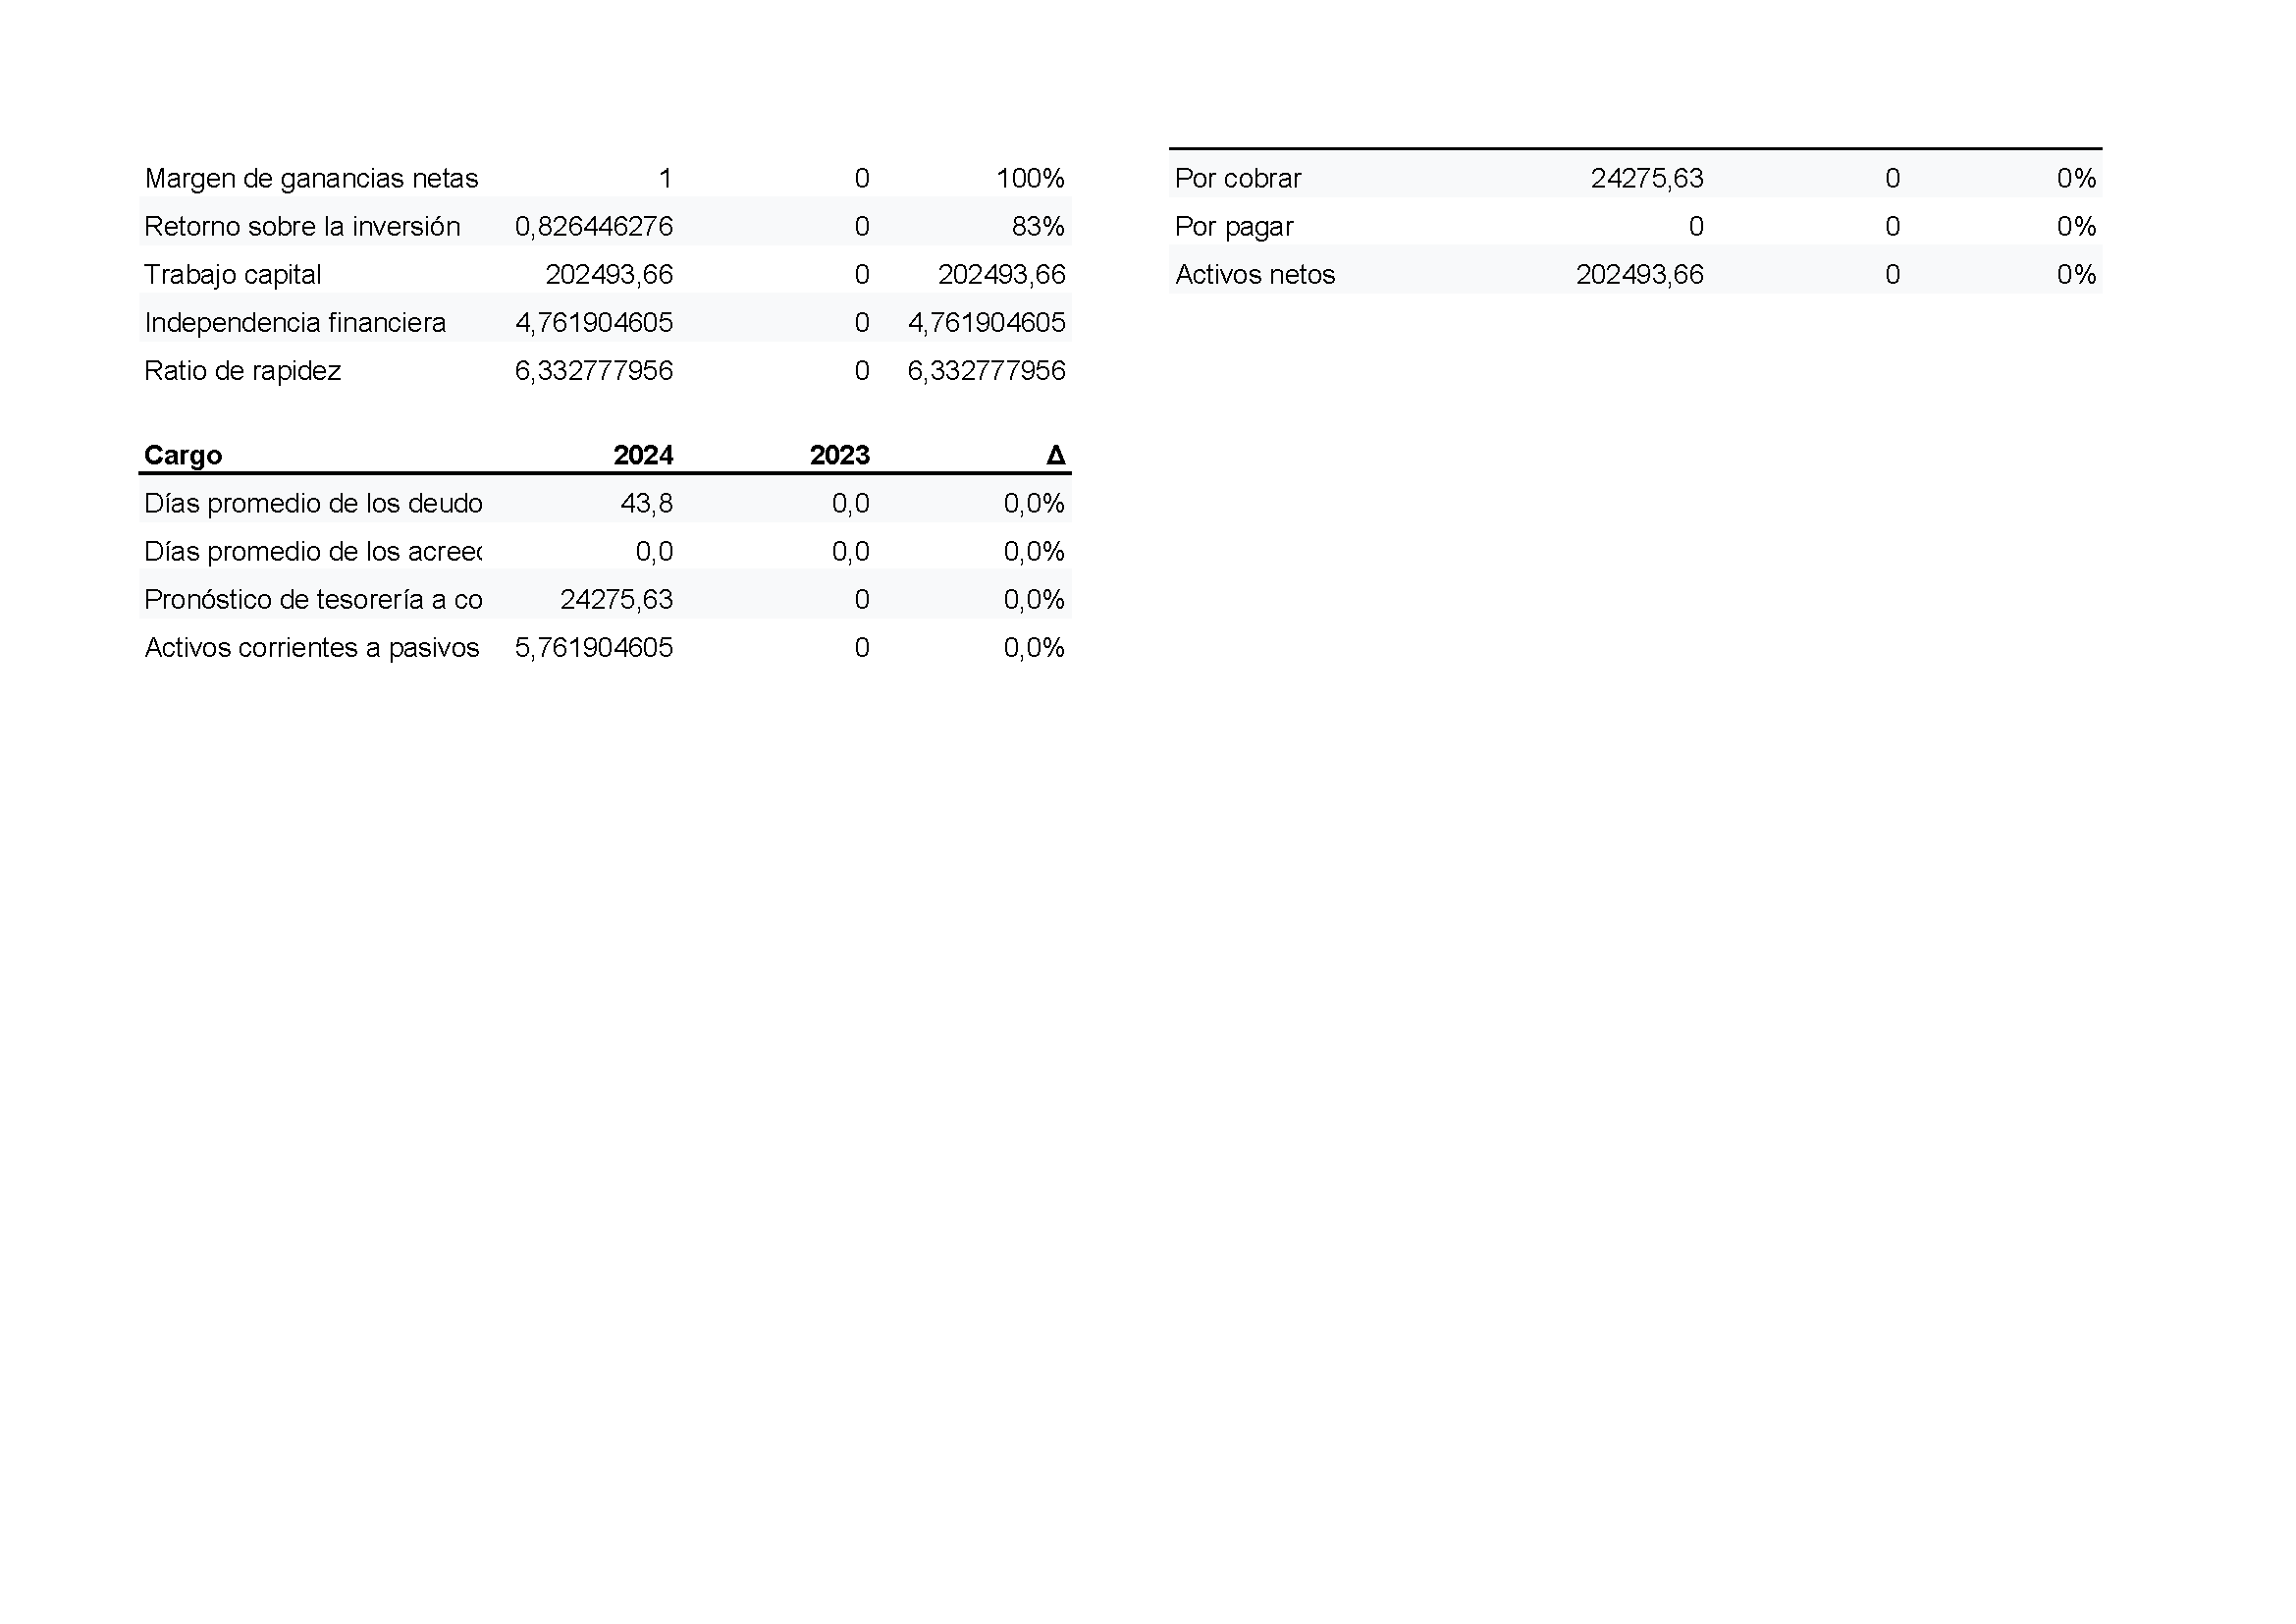
\includegraphics[width=0.8\textwidth]{./img/Contabilidad2.png}
                \caption{Resultados de la contabilidad}
            \end{figure}
        \section*{Facturación}
            \begin{figure}[H]
                \centering
                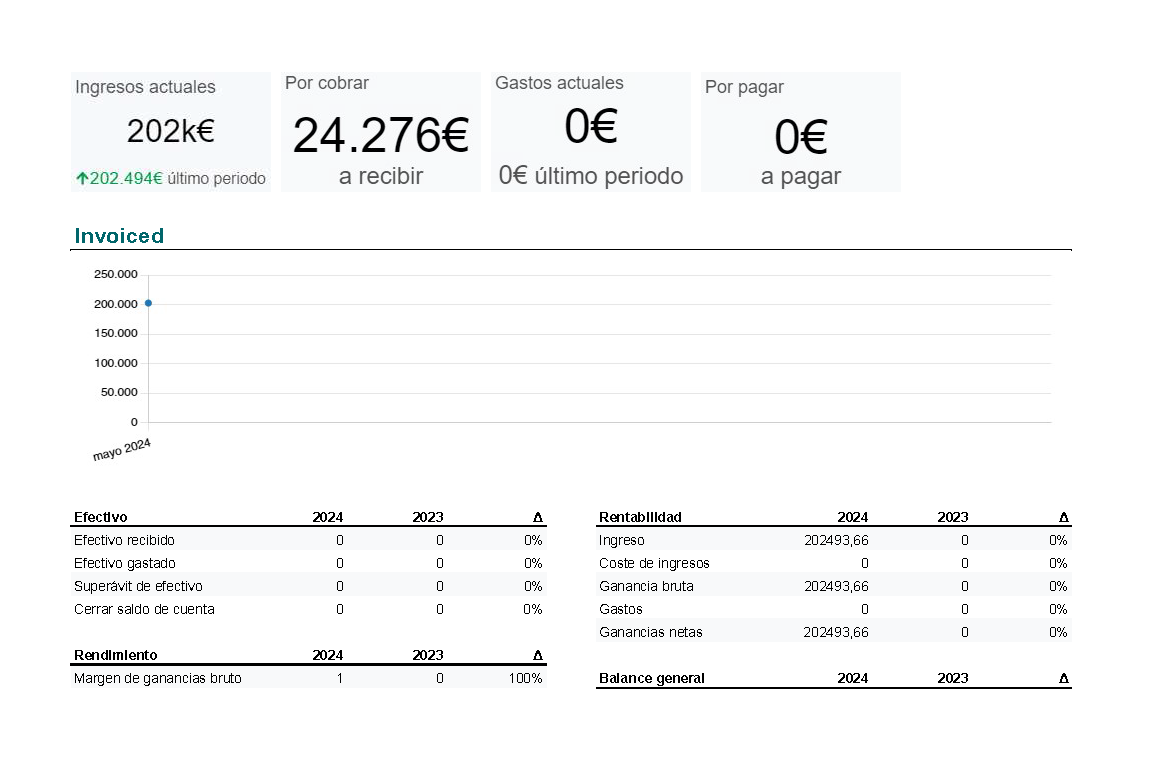
\includegraphics[width=0.55\textwidth]{./img/Facturacion1.png}
                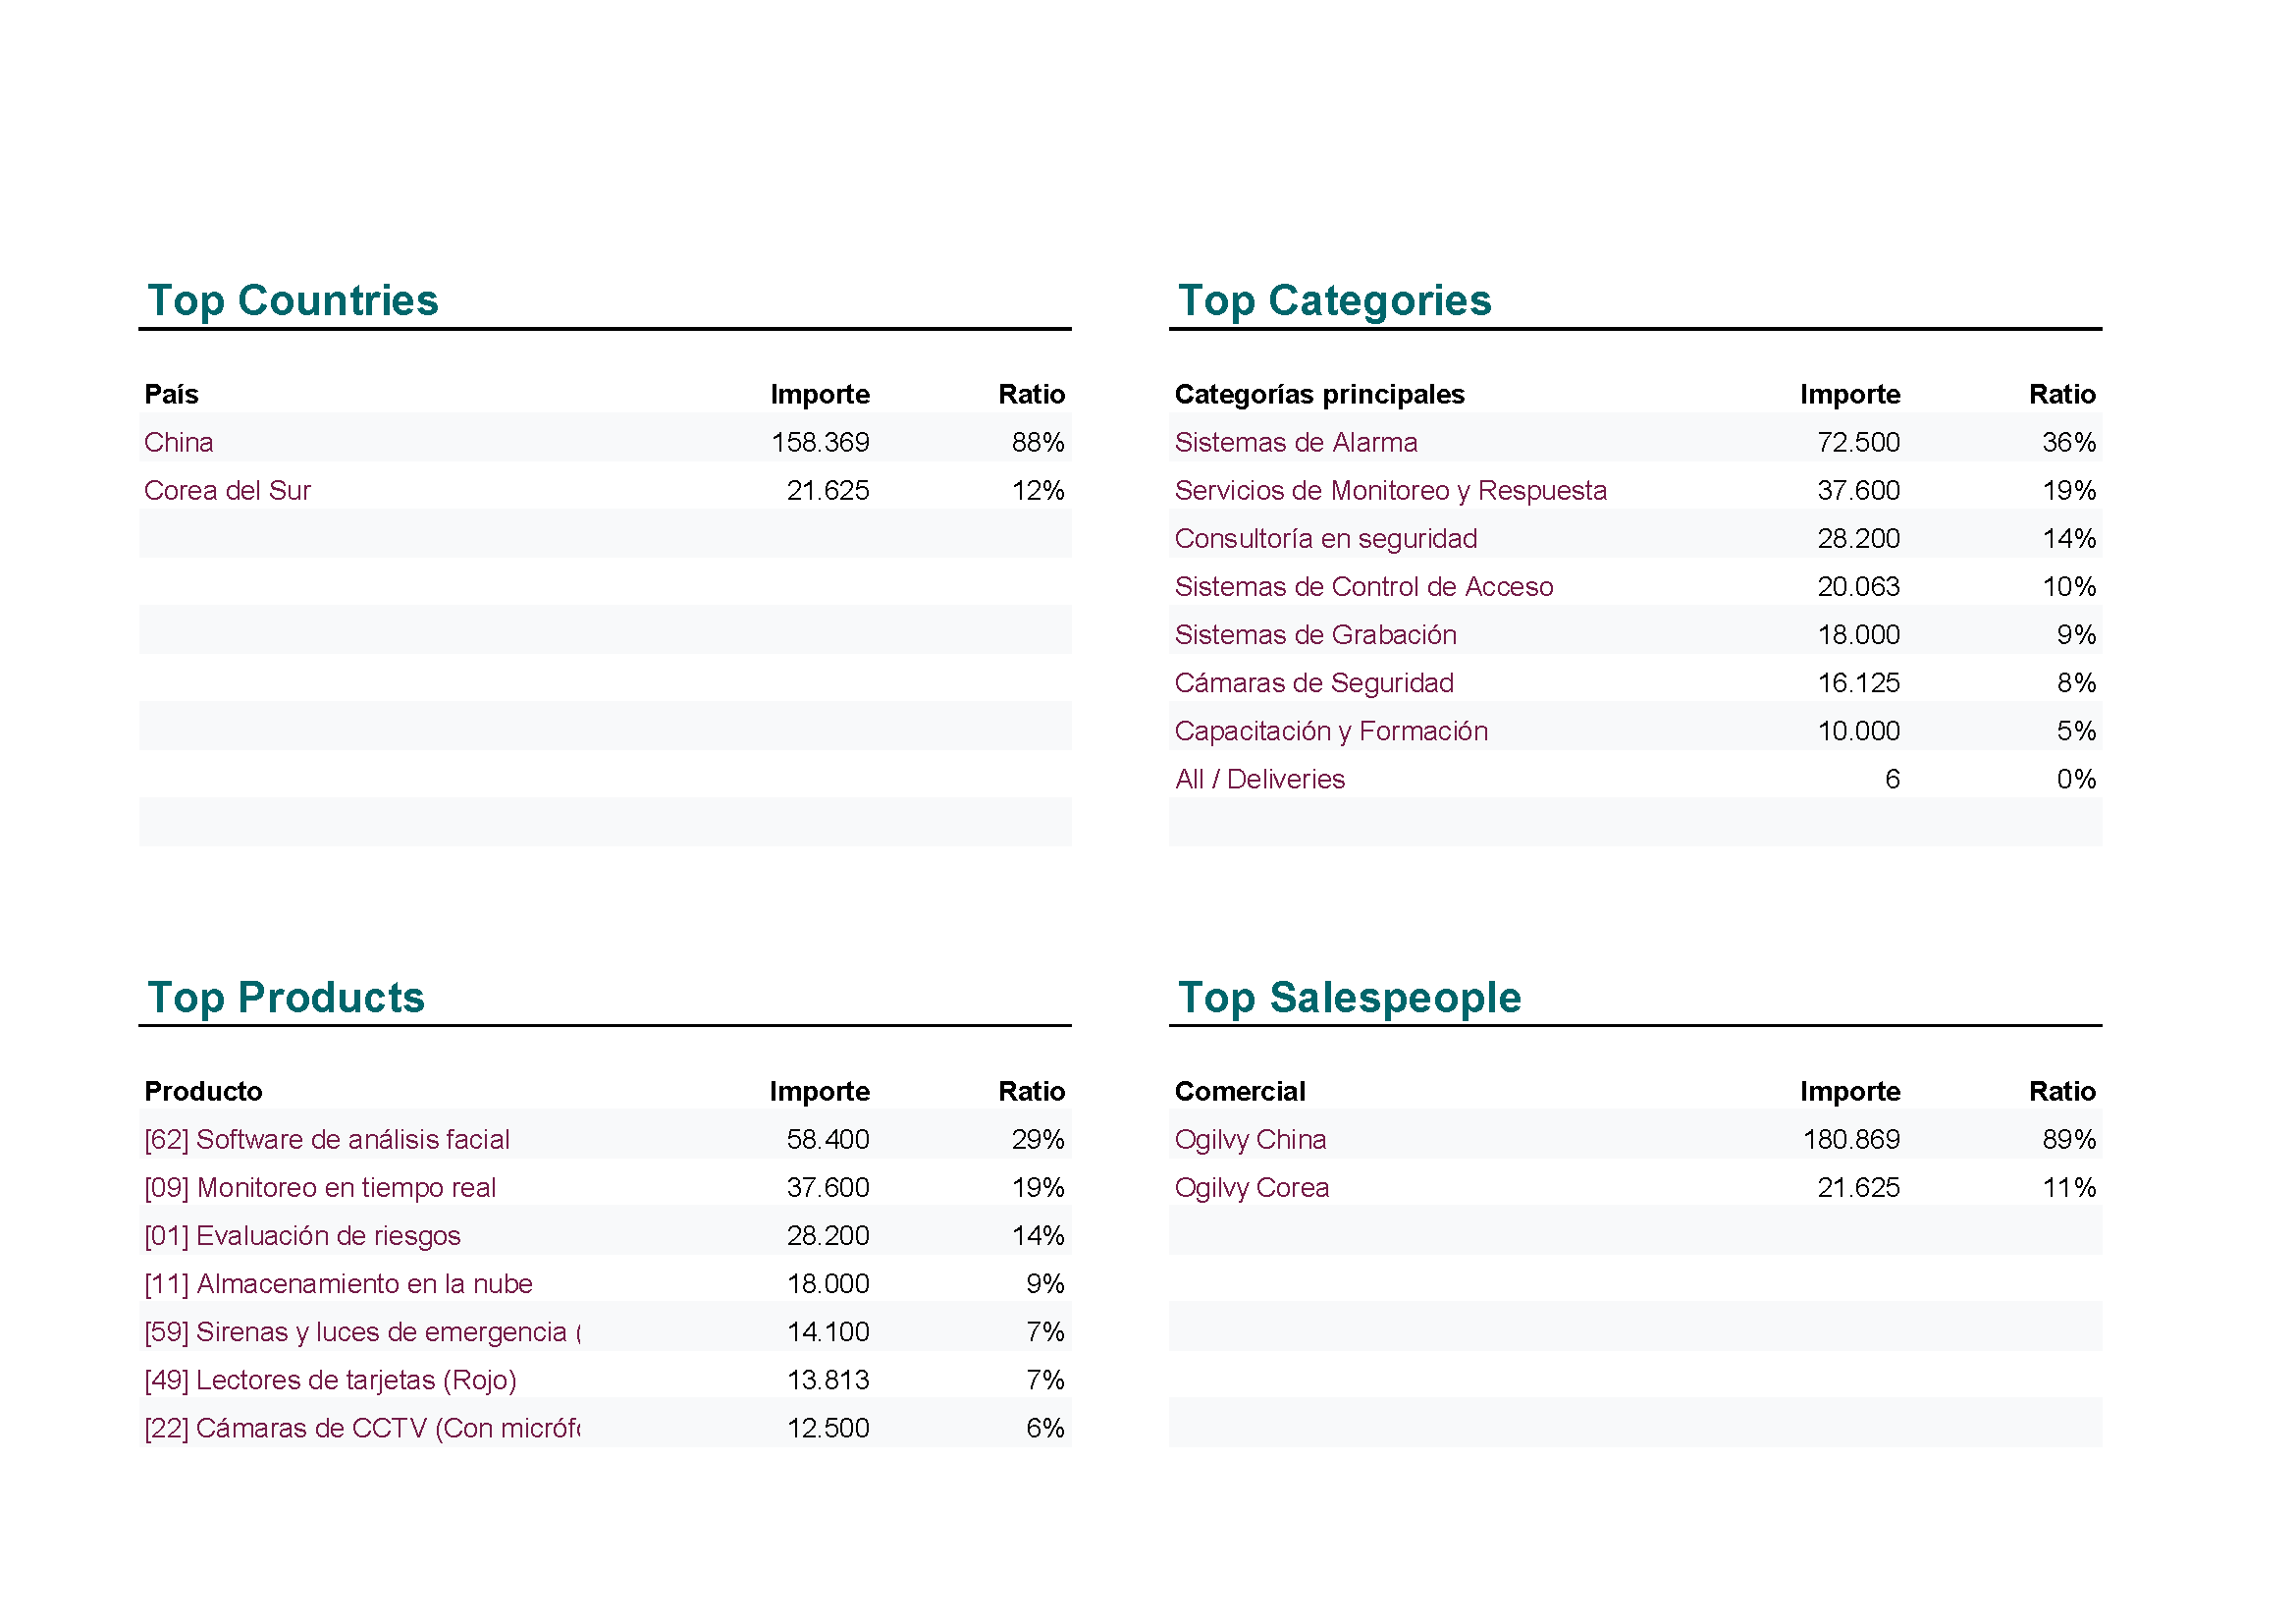
\includegraphics[width=0.55\textwidth]{./img/Facturacion2.png}
                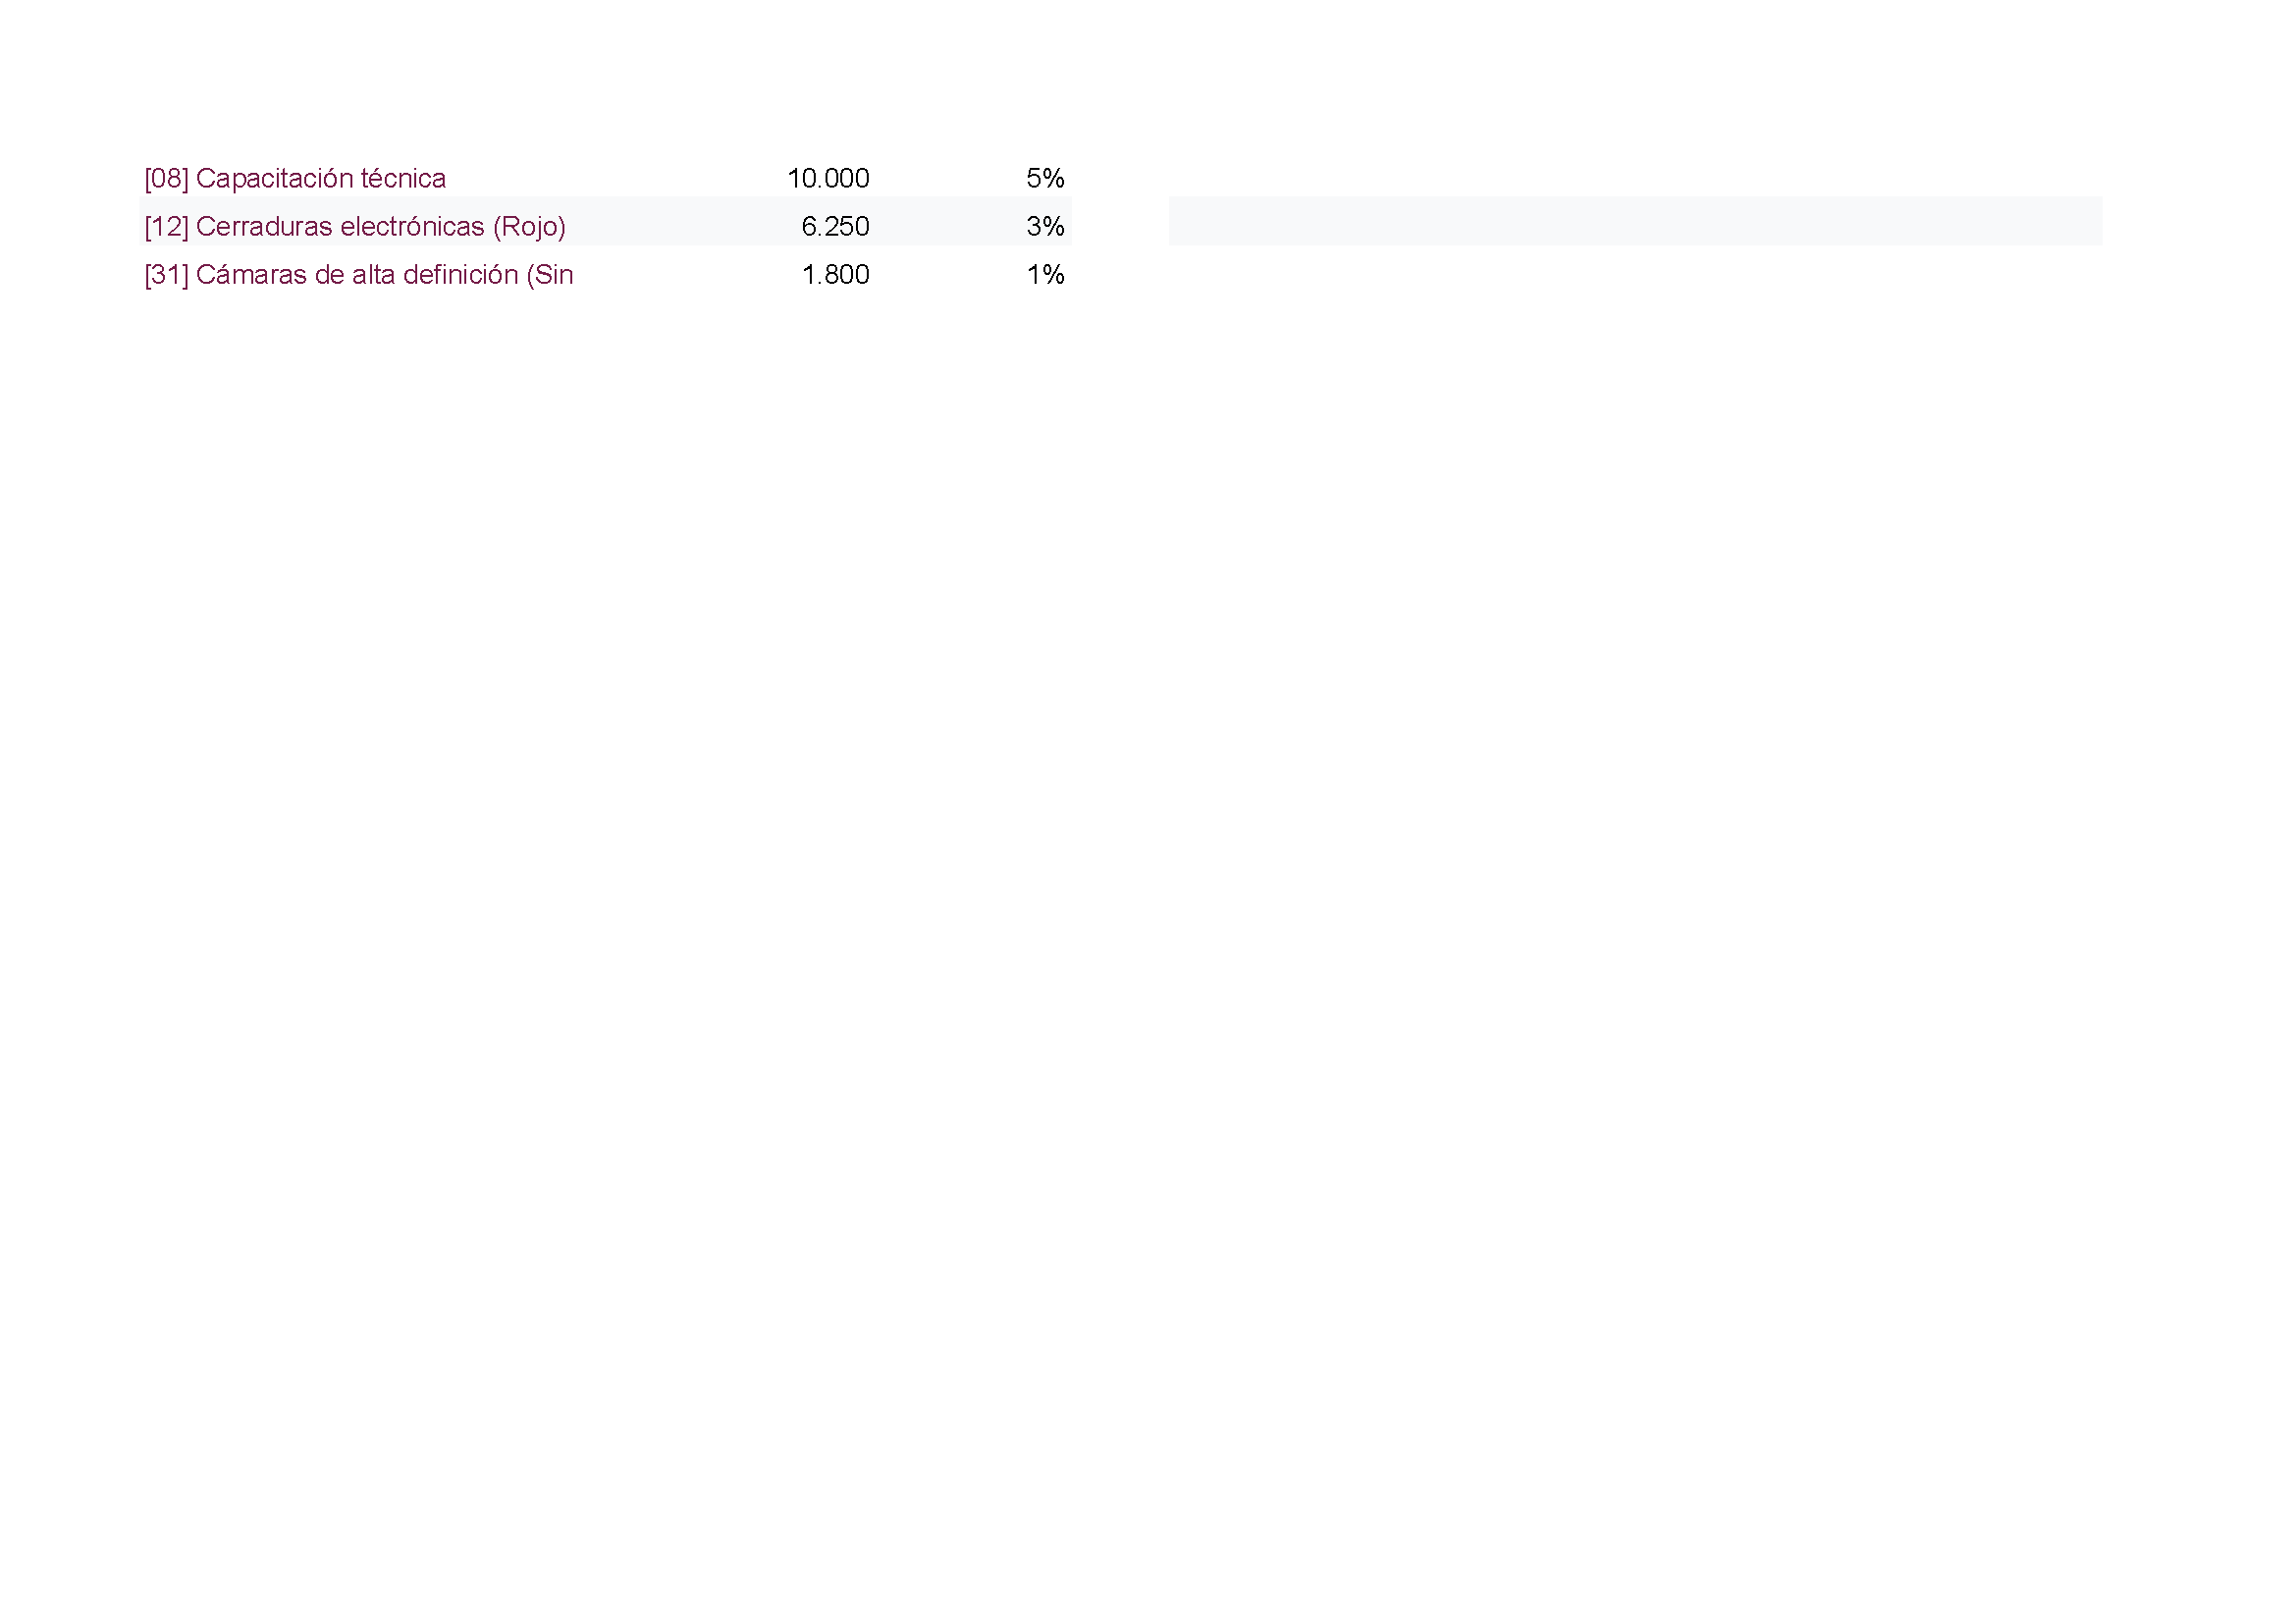
\includegraphics[width=0.55\textwidth]{./img/Facturacion3.png}
                \caption{Resultados de la facturación}
            \end{figure}
        \section*{Compra}
            \begin{figure}[H]
                \centering
                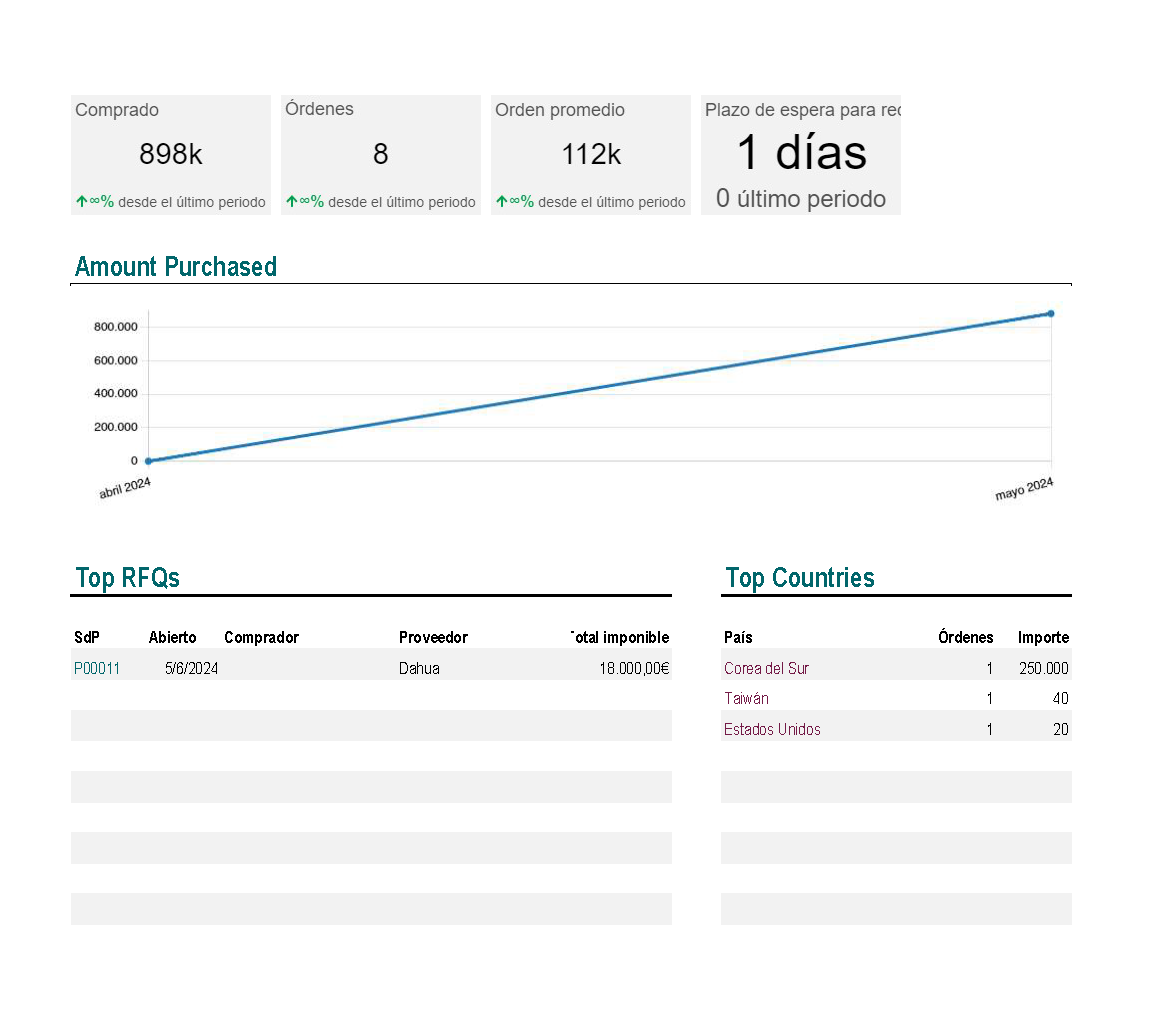
\includegraphics[width=0.55\textwidth]{./img/Compra1.png}
                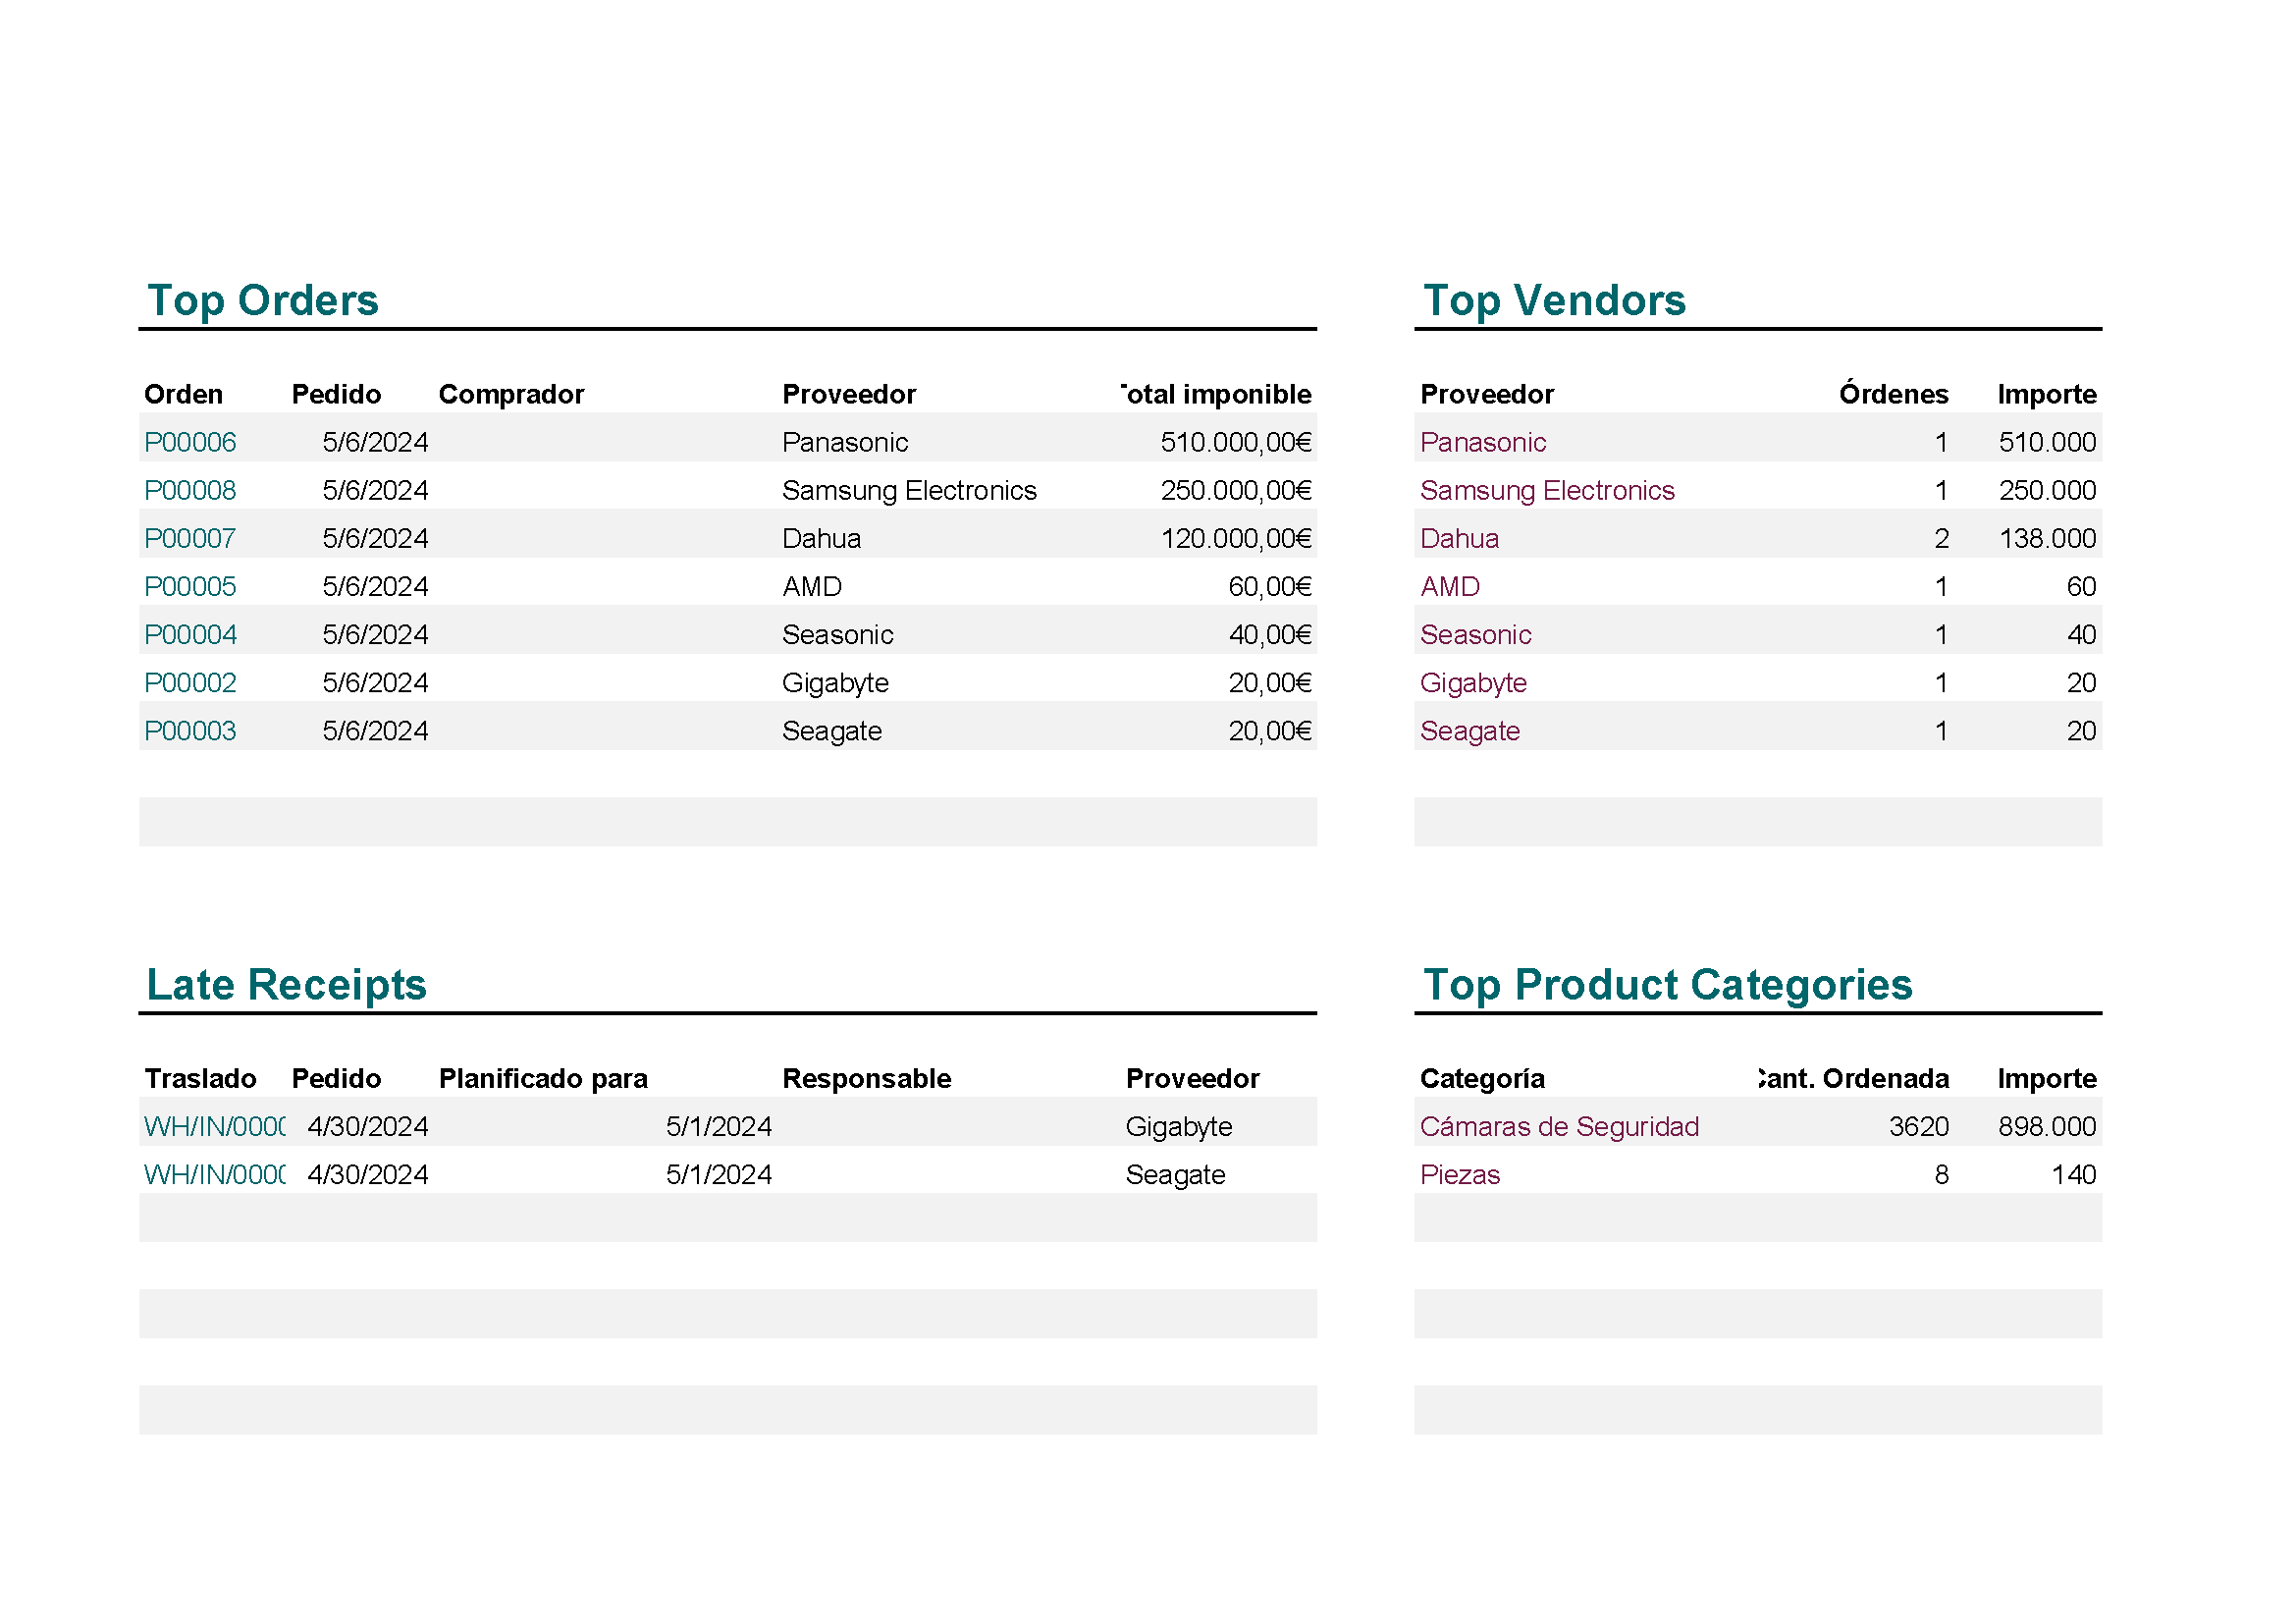
\includegraphics[width=0.55\textwidth]{./img/Compra2.png}
                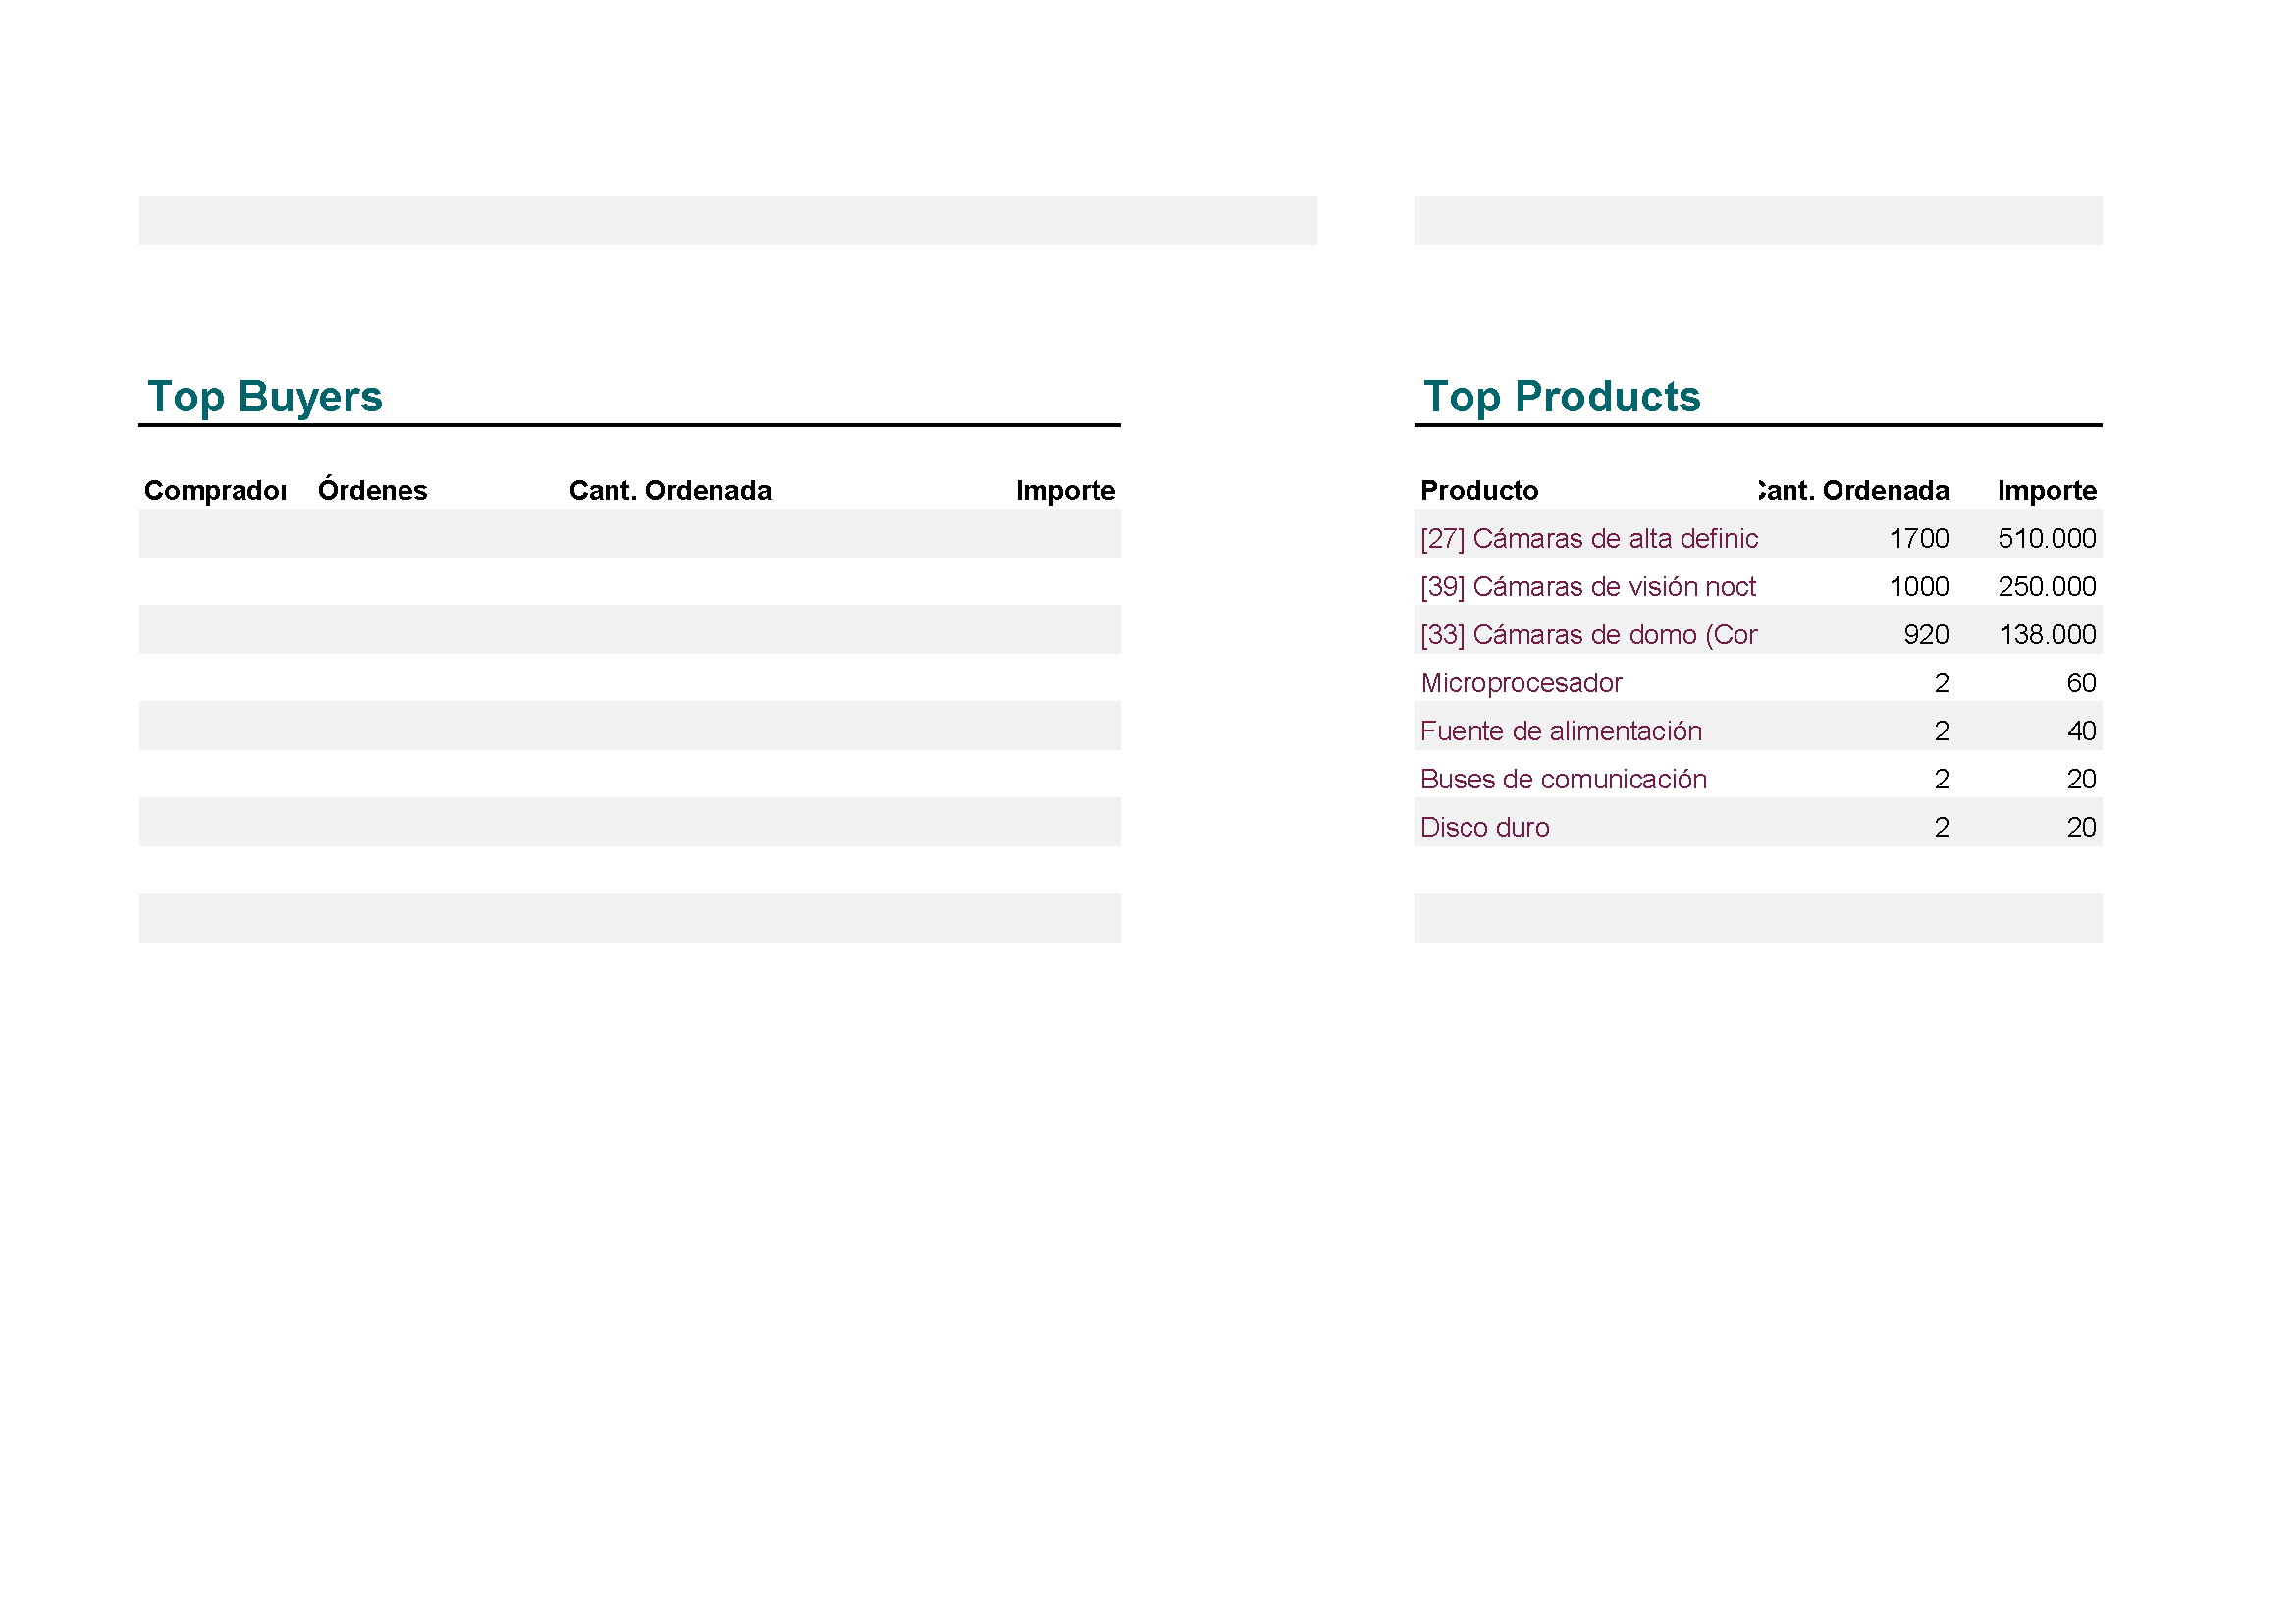
\includegraphics[width=0.55\textwidth]{./img/Compra3.png}
                \caption{Resultados de las compras}
            \end{figure}
        \section*{Proveedores}
            \begin{figure}[H]
                \centering
                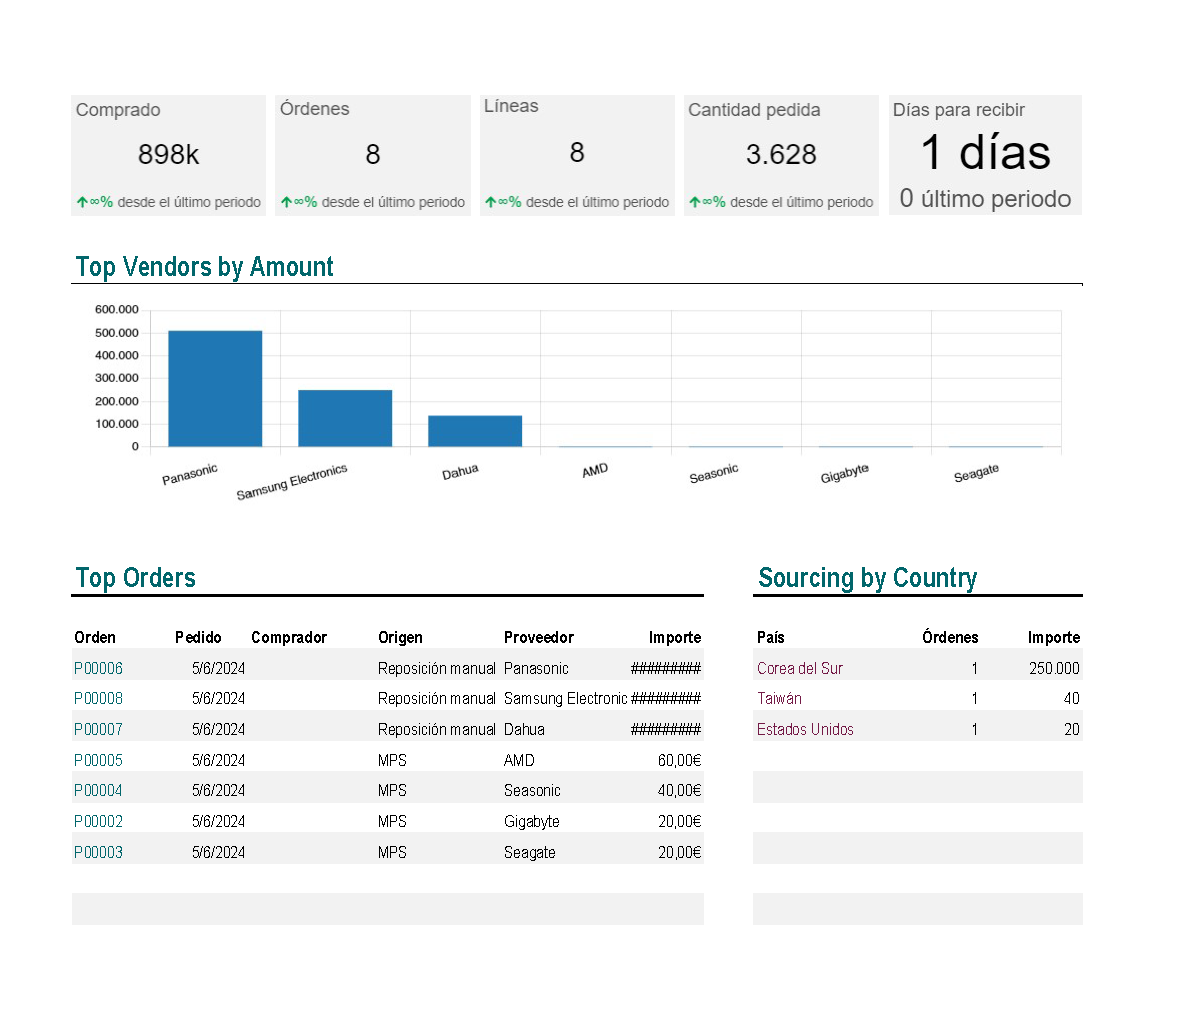
\includegraphics[width=0.8\textwidth]{./img/Proveedores1.png}
                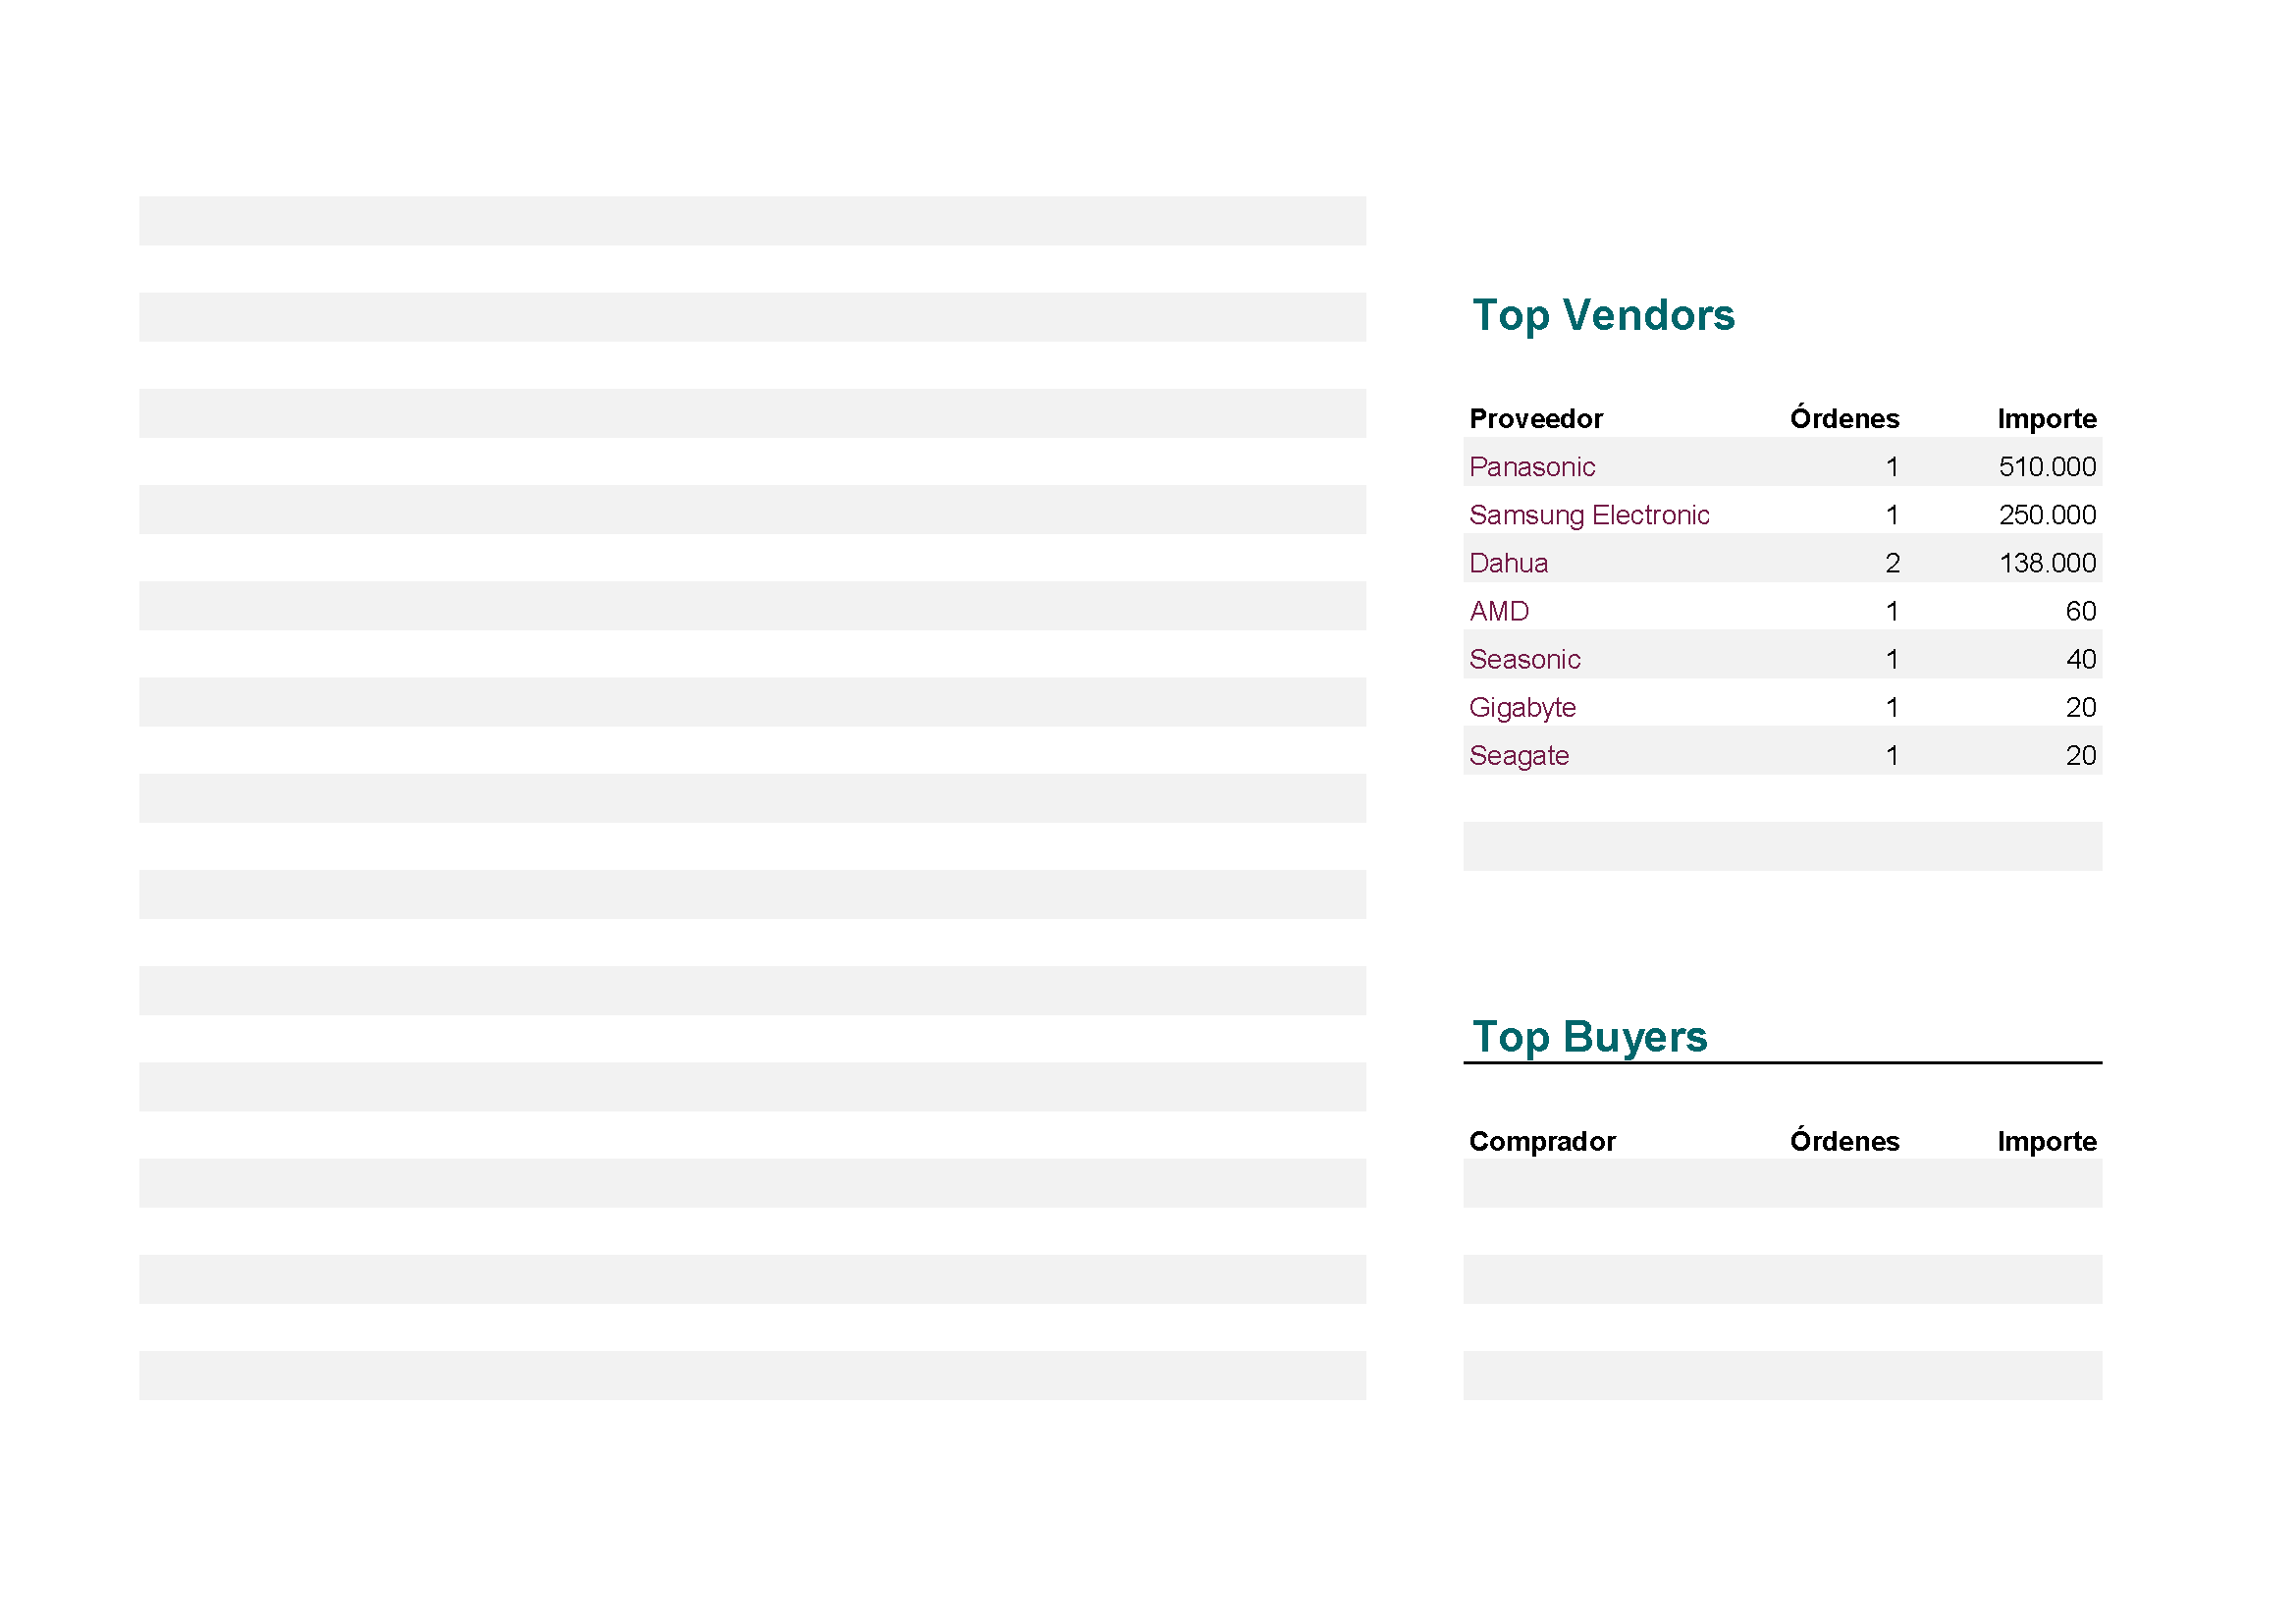
\includegraphics[width=0.8\textwidth]{./img/Proveedores2.png}
                \caption{Resultados de los proveedores}
            \end{figure}
        \section*{Inventario disponible}
            \begin{figure}[H]
                \centering
                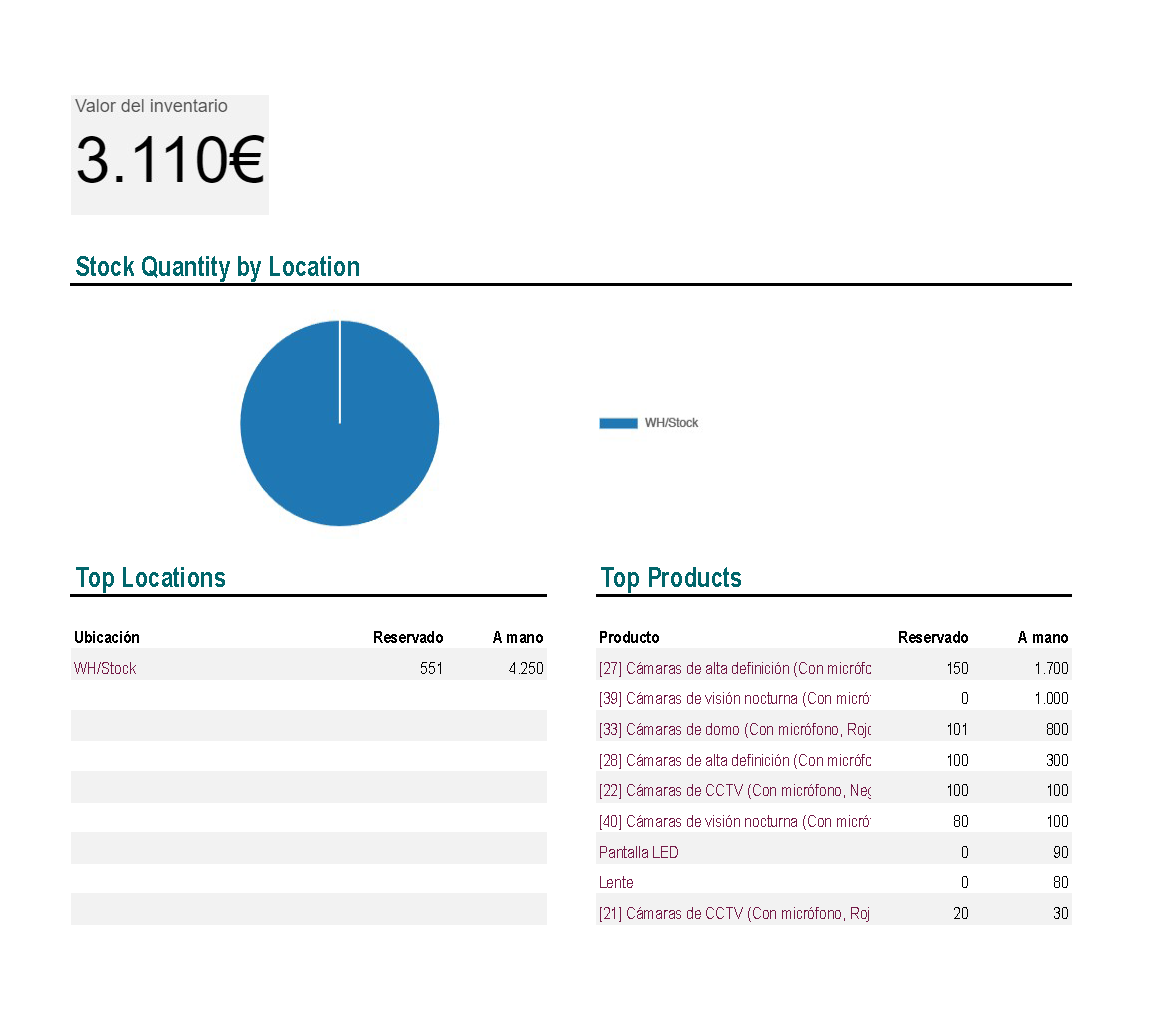
\includegraphics[width=0.8\textwidth]{./img/InventarioDisponible1.png}
                \caption{Resultados del inventario disponible}
            \end{figure}
        \section*{Flujo de inventario}
            \begin{figure}[H]
                \centering
                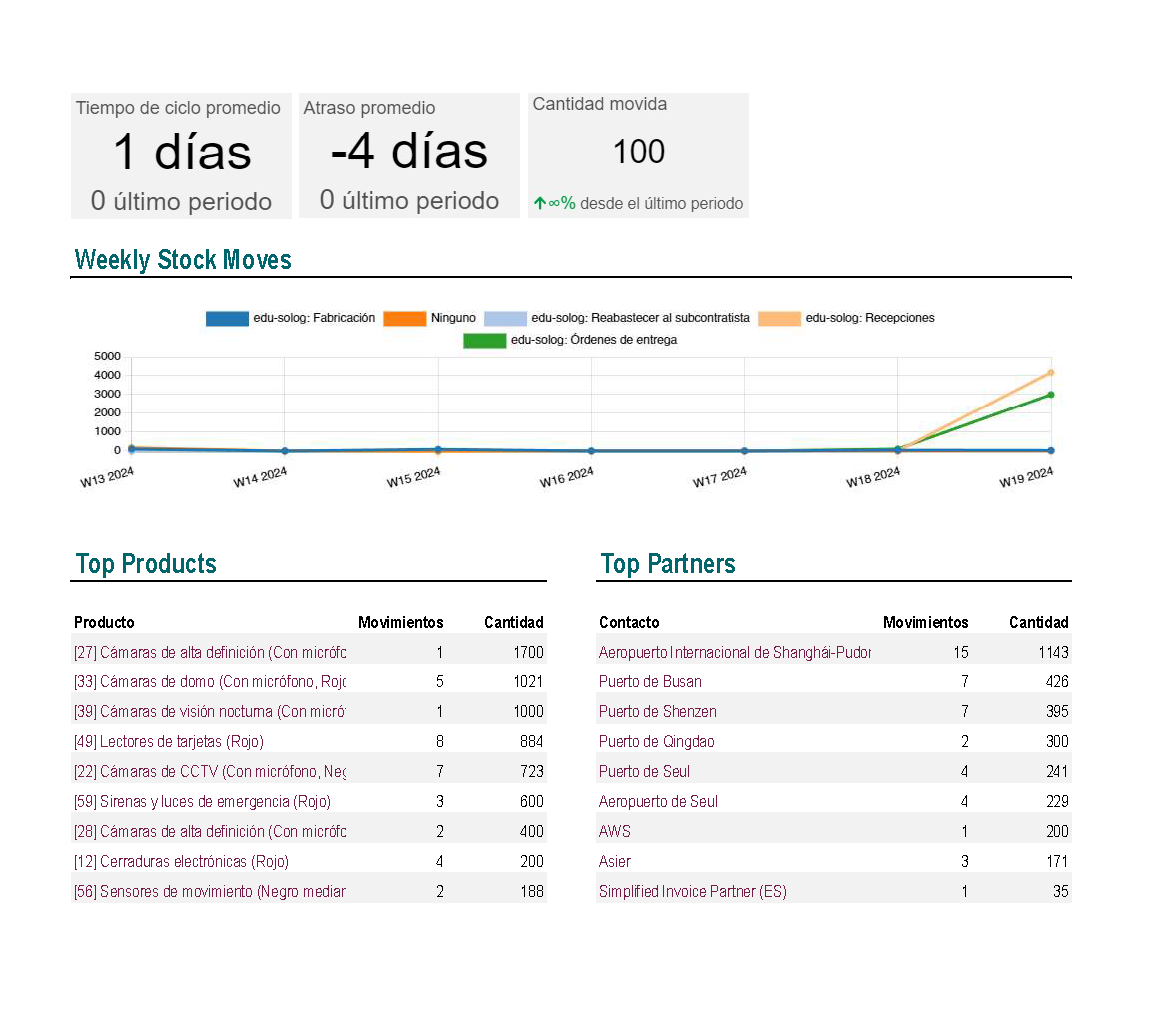
\includegraphics[width=0.8\textwidth]{./img/FlujoInventario1.png}
                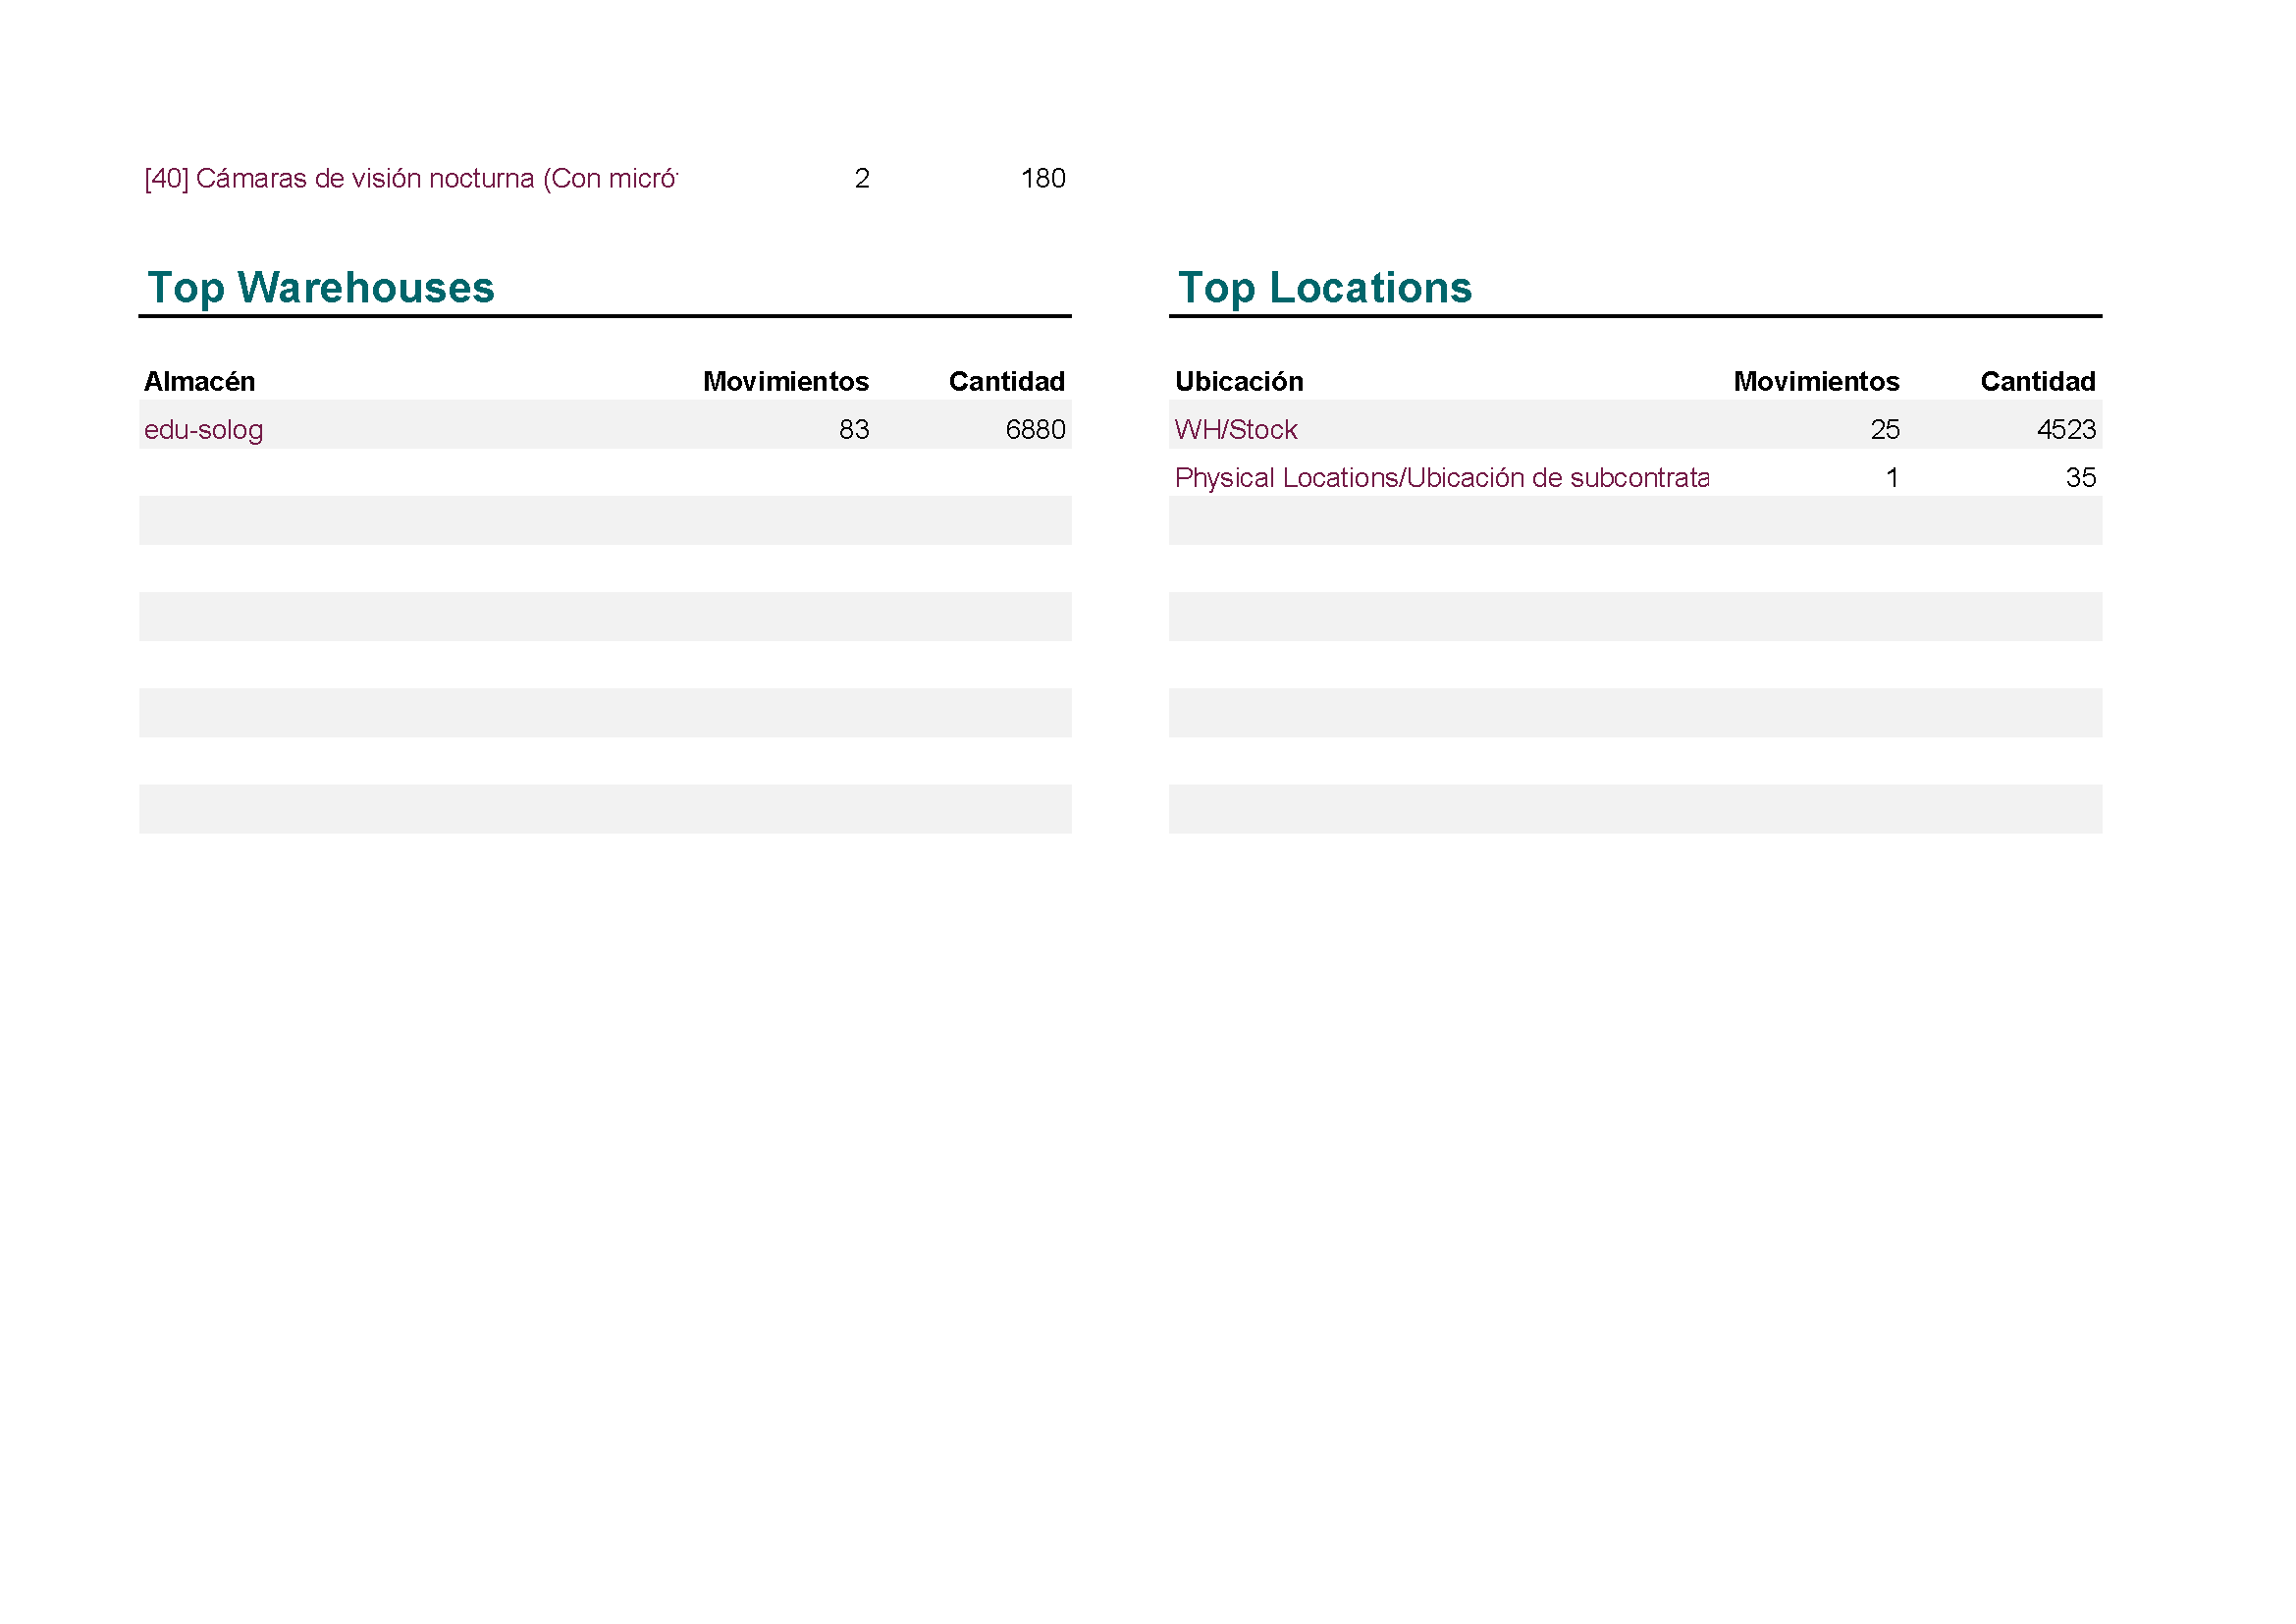
\includegraphics[width=0.8\textwidth]{./img/FlujoInventario2.png}
                \caption{Resultados del flujo de inventario}
            \end{figure}
        \section*{Fabricación}
            \begin{figure}[H]
                \centering
                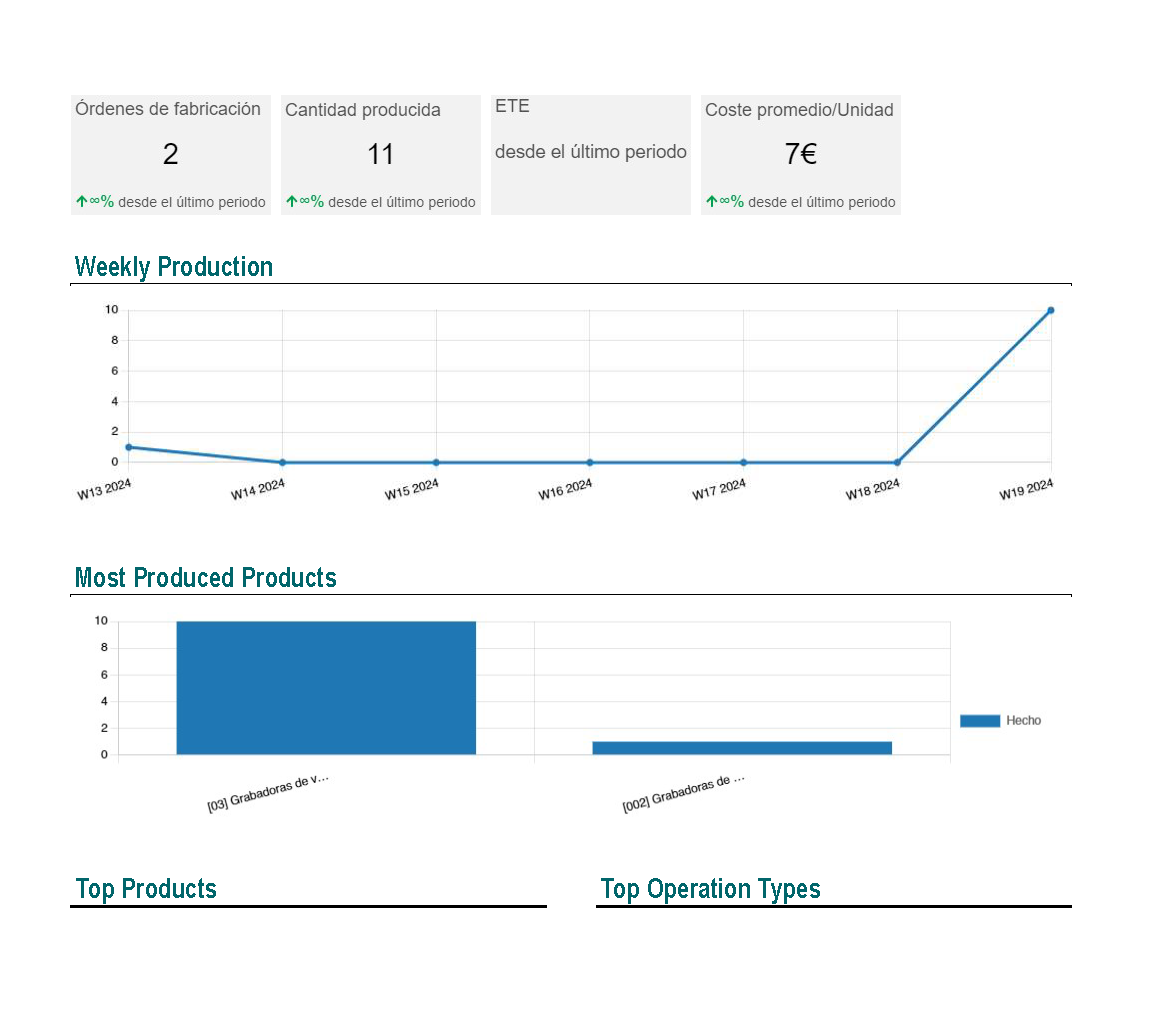
\includegraphics[width=0.8\textwidth]{./img/Fabricacion1.png}
                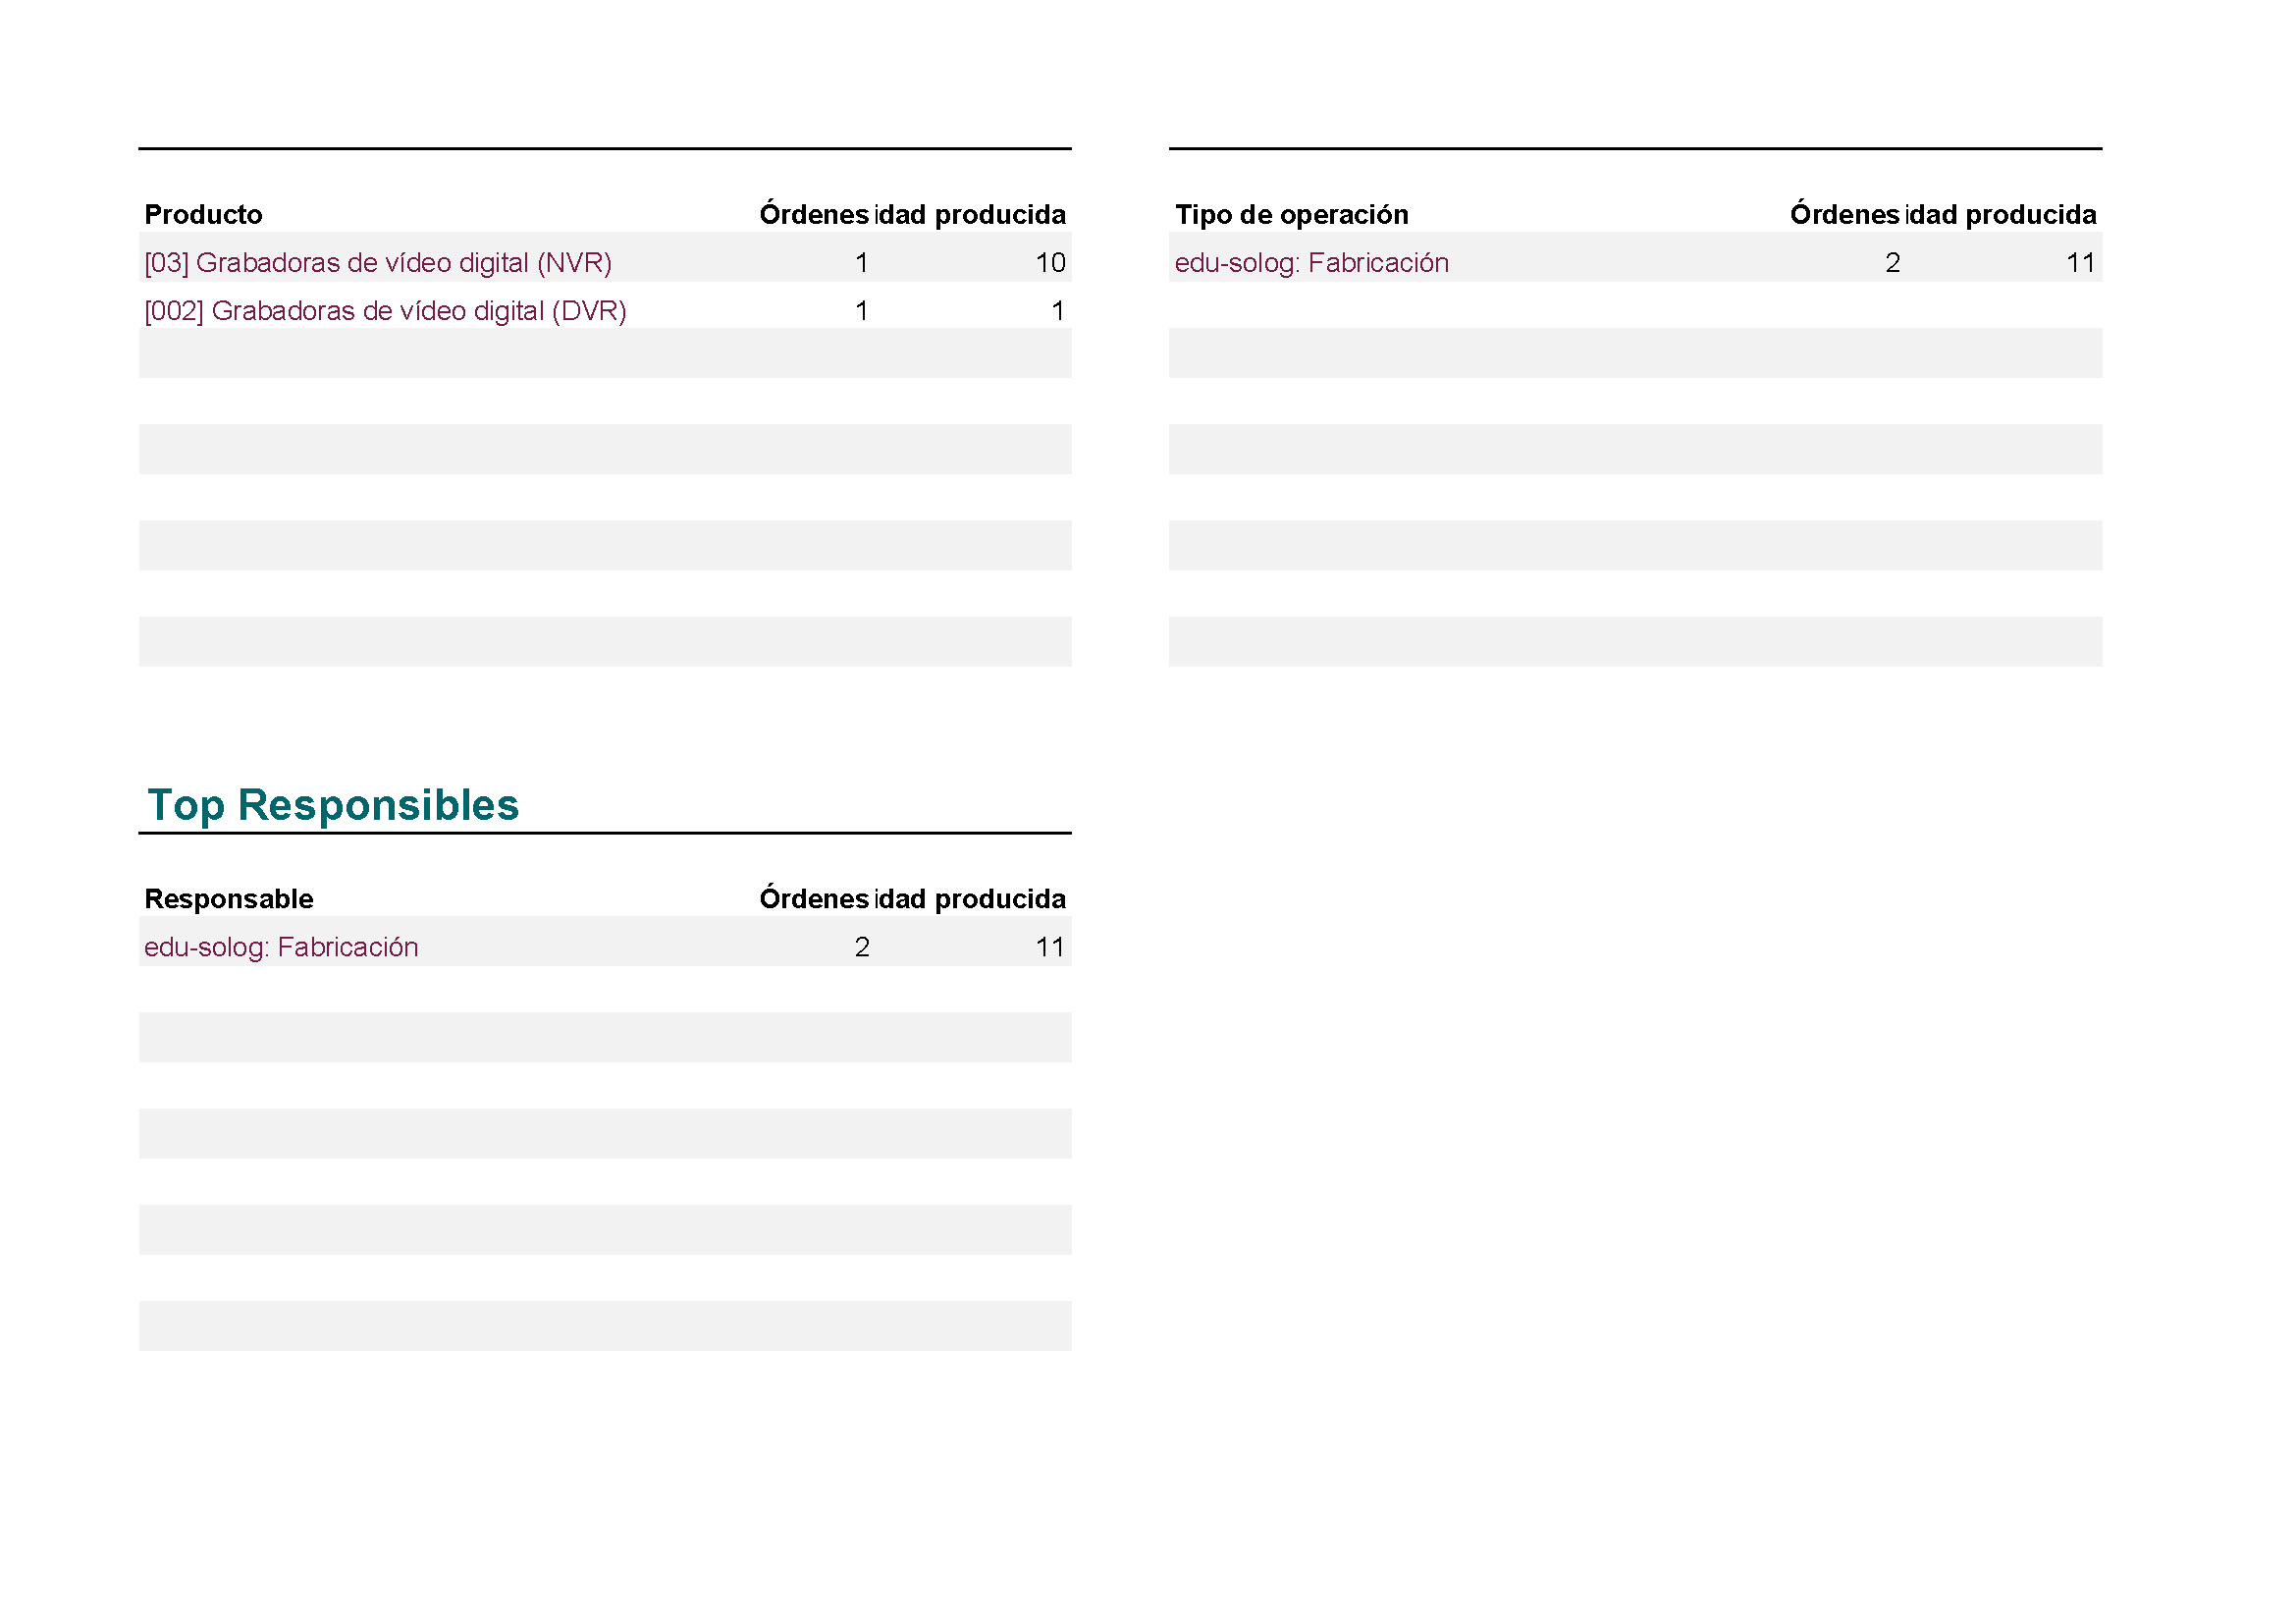
\includegraphics[width=0.8\textwidth]{./img/Fabricacion2.png}
                \caption{Resultados de las fabricaciones}
            \end{figure}
    \chapter{Checklist}
      \section*{Mínimos}
        \begin{longtable}{|p{7cm}|p{7cm}|}
          \hline
          \textbf{Punto} & \textbf{Elemento}\\
          \hline
          \hline
          1 producto distribuible (se compra para después vender). & Cámaras de CCTV  \\
          \hline
          1 producto fabricado cuya producción se planifica a través de un plan maestro de producción & Grabadoras DVR  \\
          \hline
          1 producto fabricado just in time cuya producción esté automatizada a partir del pedido de venta & Grabadoras de vídeo digital (NVR).\\
          \hline
          1 producto tipo servicio cuya venta generará la creación de un nuevo proyecto. & Evaluación de riesgos.\\
          \hline
          Al menos dos de los productos deben incluir variantes con 2 atributos. & Cámaras de CCTV y grabadoras de vídeo digital (DVR). \\
          \hline
          Cada producto fabricado tiene una lista de materiales de, al menos, 3 materias primas. & Grabadoras de vídeo digital (NVR) y grabadoras de vídeo digital (DVR)  \\
          \hline
          Se debe establecer una jerarquía de, al menos, 3 categorías de productos (aplicables también a las materias primas). & Todos los productos. \\
          \hline
          Todos los productos que se compran deben tener, al menos, dos proveedores con sus tarifas de precios definidos. &  Todos los productos\\
          \hline
          Todos los productos que se venden deben tener, al menos, dos tarifas de precios configuradas. & Dos listas para los productos a vender. \\
          \hline
          Se deben definir, al menos, dos equipos de ventas con un responsable y tres comerciales a su cargo. & Equipo de China y Equipo de Corea. \\
          \hline
          Deben existir, al menos, 5 oportunidades de venta en curso (en distintos estados), 5 pedidos de venta en fase de presupuesto y 5 pedidos de venta confirmados. Estos pedidos deberán estar distribuidos entre los distintos equipos de ventas y empleados. El seguimiento de estos pedidos incluirá la definición de tareas como envío de emails, envío de documentación y planificación de reuniones. & Confirmadas: S00036, S00031, S00029, S00030, S00024; Curso: S00022, S0041, S00044, S0043, S00034; Presupuestos: S00038, S00037, S00033, S00032, S00050\\
          \hline
          Al menos dos de los presupuestos ofertados deberán incluir descuentos en la línea de pedido independientemente de la tarifa aplicada. & Presupuesto S00038, S00022, S00031 \\ 
          \hline
          Se definirán costes de envío en función de la zona geográfica. & Internacional Express, China Express, Corea Express, Presupuesto S00044, S00038, S00024\\
          \hline
          Se deben generar distintas órdenes de fabricación como consecuencia de las ventas realizadas de los distintos productos: provenientes de ventas de productos just-in-time o de la ejecución del plan maestro de producción. & Las ordenes de fabricación de NVR y DVR.\\
          \hline
          De forma similar, deben aparecer las órdenes de compra derivadas de los distintos tipos de abastecimiento contemplados. & P00002-P00008. \\
          \hline
          El proyecto asociado al producto de tipo servicio debe tener un mínimo de 5 tareas que se asignan a responsables de, al menos, dos departamentos distintos. & Servicio: Evaluación de riesgos, Departamentos: Operaciones, Atención al Cliente, Administración y Finanzas \\
          \hline
          Se habrán definido, al menos, 3 etapas en la ejecución de los proyectos. & Evaluación de riesgos: Estudio, Testeo, Documentación. \\
          \hline
          Debe haber, al menos, dos ventas del producto de tipo servicio y los proyectos asociados deberán crearse automáticamente. Habrá tareas distribuidas a lo largo de las etapas, en función de su grado de desarrollo. El seguimiento de estos proyectos incluirá la definición de tareas como envío de emails, envío de documentación y planificación de reuniones. & Servicio: Evaluación de riesgos; Proyectos: S00031, S00036 \\
          \hline
          Las tareas se irán ejecutando incorporando las horas de trabajo de los empleados a cada tarea. & Evaluación de riesgos proyecto. \\
          \hline
          Los permisos de acceso de los empleados deberán ajustarse a sus funciones (ver sólo los módulos que les competen) y su nivel de decisión (el responsable puede ver la información de los empleados a su cargo, pero no los de otros empleados). & Se han ajustado los permisos de los trabajadores\\
          \hline
          Todos los módulos implementados deberán generar informes con información sobre los distintos productos/equipos de ventas/proveedores/clientes. & Hemos añadido el modulo Tablero para ello. \\
          \hline
          \caption{Checklist de los puntos a comprobar}
        \end{longtable}
      \clearpage\section*{Extras}
        \begin{itemize}
          \item Creación de la tienda online como implementación de módulo extra
          \item Definición de iniciativas de venta en el CRM
          \item Definición de permisos avanzados de usuarios distintos a los vistos en clase
        \end{itemize}
    \chapter{Anexo}
      \section{Gantt}
        \begin{figure}[H]
          \centering
          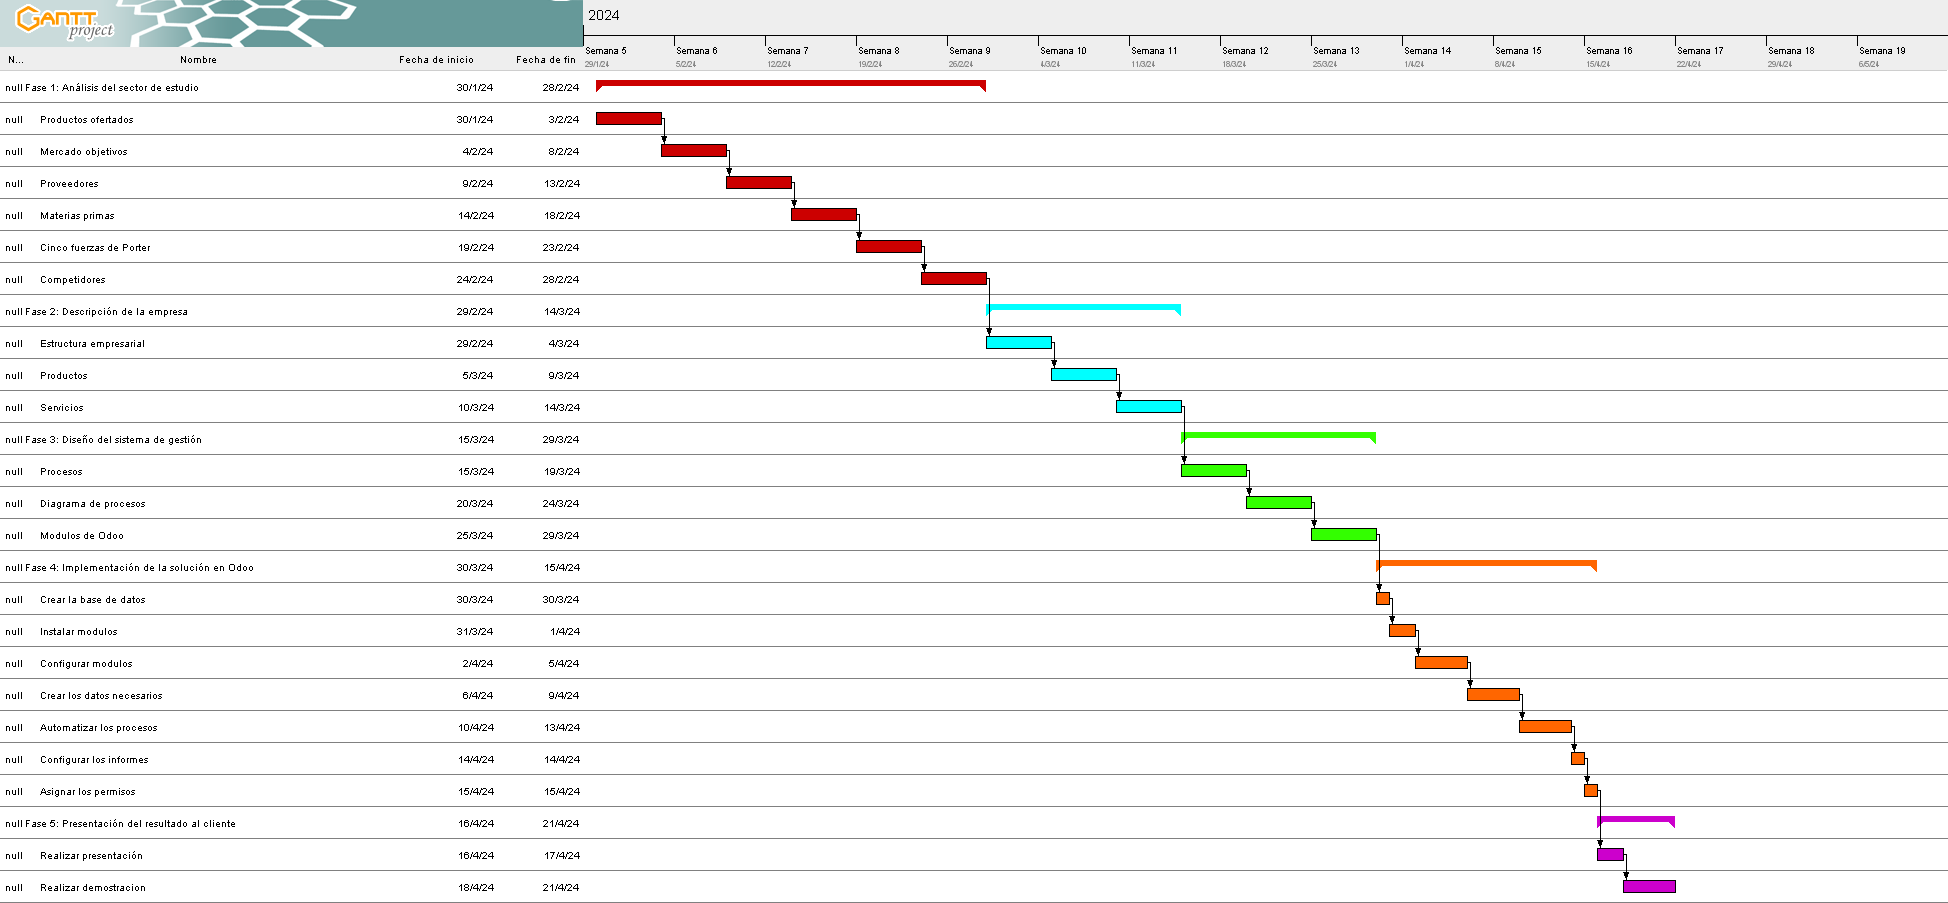
\includegraphics[width=1\textwidth]{./img/gantt.png}
          \caption{Diagrama de Gantt}
        \end{figure}
    \bibliographystyle{plain}
    \bibliography{bibliografia.bib}
\end{document}